%==============================================================================
% DRAFT -- single-file working copy.   Compile: biber draft; latexmk -pdf draft.tex
%
% >>> THIS FILE IS THE LIVE COPY. Edit here. <<<
% chapters/*.tex and main.tex are FROZEN and now out of date. Do not edit them
% until the split-back below has happened.
%
% SPLIT-BACK PLAN (when the official EPCC template arrives / drafting settles):
%   Each chapter is preceded by a  "% ===== FILE: chapters/xxx.tex ====="  marker.
%   Cut at those markers into the matching files under chapters/, drop this
%   preamble (main.tex already has it), and main.tex compiles unchanged.
%   Keep \chapter/\section as-is: the structure is already the dissertation's.
%
% Draft settings: `oneside` = no blank pages between chapters. The printed
% submission uses [11pt,a4paper,twoside,openright] + geometry bindingoffset=6mm.
%==============================================================================
\documentclass[11pt,a4paper,oneside]{report}

%------------------------------------------------------------------ engine-safe fonts
\usepackage{iftex}
\ifPDFTeX
  \usepackage[utf8]{inputenc}
  \usepackage[T1]{fontenc}
  \usepackage{lmodern}
\else
  \usepackage{fontspec}
\fi

%------------------------------------------------------------------ layout & graphics
\usepackage[a4paper,margin=2.5cm]{geometry}
\usepackage{graphicx}
% figures/ ONLY. Never point this at the analysis/ tree: reorganising the plots
% directory then silently breaks the build. Refresh with ./sync_figures.sh.
\graphicspath{{figures/}}
\usepackage{booktabs}
% array: ragged-right p columns, so the long paths in the evidence index wrap
% without stretching the inter-word space past the column edge.
\usepackage{array}
\newcolumntype{L}[1]{>{\raggedright\arraybackslash}p{#1}}
\usepackage{amsmath,amssymb}
\usepackage{listings}
\usepackage{microtype}
\usepackage{csquotes}

%------------------------------------------------------------------ float placement
% Every figure and table is declared immediately after the paragraph that first
% discusses it, so the aim is simply to stop LaTeX deferring them further than
% necessary. Three things do that, and none of them touches the text:
%   flafter   -- a float never surfaces on a page BEFORE its declaration point.
%   placeins  -- \FloatBarrier at each \section, so a float cannot escape into a
%                later section than the one that introduces it.
%   fractions -- the defaults reserve so much of the page for text that a
%                half-page figure is often refused a slot it would in fact fit.
\usepackage{flafter}
\usepackage[section]{placeins}
% placeins only barriers at \section. Since the 2026-08-03 restructure the 2D/3D
% boundary inside Chapter 4 is a \subsection, and a 2D figure was drifting past the
% start of the 3D subsection, so the barrier is lowered one level.
\let\OldSubsection\subsection
\renewcommand{\subsection}{\FloatBarrier\OldSubsection}
\renewcommand{\topfraction}{0.9}       % default 0.7
\renewcommand{\bottomfraction}{0.7}    % default 0.3
\renewcommand{\textfraction}{0.1}      % default 0.2
\renewcommand{\floatpagefraction}{0.75}% default 0.5
\setcounter{topnumber}{3}              % default 2
\setcounter{bottomnumber}{2}           % default 1
\setcounter{totalnumber}{4}            % default 3

%------------------------------------------------------------------ bibliography
\usepackage[backend=biber,style=numeric-comp,sorting=none]{biblatex}
\addbibresource{references.bib}

%------------------------------------------------------------------ links (load late)
\usepackage[hidelinks]{hyperref}
\usepackage[capitalise]{cleveref}

\emergencystretch=2em

\title{Hybrid MPI+OpenMP Performance of PETSc Krylov Solvers on ARCHER2}
\author{Leyan Li}
\date{August 2026}

\begin{document}

% ===== FILE: chapters/00_frontmatter.tex =====
\pagenumbering{roman}
\hypersetup{pageanchor=false}
\begin{titlepage}
\centering
\vspace*{2cm}
{\LARGE\bfseries Hybrid MPI+OpenMP Performance of PETSc\\[0.3em]
Krylov Solvers on ARCHER2\par}
\vspace{2cm}
{\Large Leyan Li\par}
\vspace{1cm}
{\large MSc in High Performance Computing\par}
{\large EPCC, University of Edinburgh\par}
\vspace{1cm}
{\large August 2026\par}
\vfill
{\normalsize A dissertation submitted in partial fulfilment\\
of the requirements for the degree of\\
Master of Science.\par}
\end{titlepage}
\hypersetup{pageanchor=true}
\clearpage

\chapter*{Abstract}
\addcontentsline{toc}{chapter}{Abstract}
PETSc can combine MPI ranks with OpenMP threads, but the best balance depends on the
solver, decomposition and concurrency. This dissertation compares four full-node layouts
on ARCHER2: flat MPI and hybrid layouts with two, four or eight threads per rank. Matched
2D and 3D Poisson benchmarks cover 5.0--164.6 million unknowns on 1--32 nodes. Each formal
configuration is run three times, and every run performs one warm-up solve that builds the
GAMG hierarchy, followed by 19 timed solves that reuse it. Eleven admitted size--node pairs
form two weak-scaling chains at approximately constant work per core.

In 2D, hybrid layouts improve relative to flat MPI as concurrency grows, and four of the six
layout--chain series improve at every step. $64\times2$ is faster per iteration than flat MPI
at all 11 pairs and reaches 13.1\% higher raw throughput at 164.56 million unknowns on 32
nodes. The 3D advantage is larger, reaching 33.2\%, but no series improves at every step and
the best layout changes with scale and node count. Eight threads per rank wins no
weak-scaling point in either dimension.

A matched extension holds the problem near 20 million unknowns while scaling from one to
32 nodes. All four 2D layouts still improve at 4096 cores. In 3D, flat MPI stops improving
and starts getting slower after eight nodes, and the intermediate layouts after 16, while
$16\times8$ is still improving at 32 and is $3.81\times$ faster than flat MPI there. PETSc event data associate the hybrid
advantage with lower exposure to halo exchange and global reduction. Eleven Linaro MAP
profiles show an opposing rise in OpenMP-runtime waiting as threads replace ranks, while
threaded BLAS accounts for at most 2.1\% of core time during the solve. These measurements
locate the software costs but do not establish the hardware mechanism.

\chapter*{Acknowledgements}
\addcontentsline{toc}{chapter}{Acknowledgements}
% TODO: supervisor, EPCC, ARCHER2 access.

\tableofcontents
\listoffigures
\listoftables
\clearpage

\chapter*{Abbreviations}
\addcontentsline{toc}{chapter}{Abbreviations}
\begin{tabular}{@{}l p{0.76\textwidth}@{}}
  AMG    & Algebraic multigrid \\
  BLAS   & Basic Linear Algebra Subprograms, the standard interface for dense
           vector and matrix operations \\
  CCD    & Core Complex Die, two CCXs on an AMD Zen 2 processor \\
  CCX    & Core Complex, four cores sharing one 16\,MB L3 cache \\
  CG     & Conjugate gradients \\
  GAMG   & PETSc's algebraic multigrid preconditioner (\texttt{PCGAMG}) \\
  GMRES  & Generalised minimal residual method, PETSc's default Krylov solver \\
  ICC    & Incomplete Cholesky factorisation \\
  KSP    & PETSc's Krylov subspace solver object \\
  LAPACK & Linear Algebra PACKage, the dense factorisation layer above BLAS \\
  LibSci & HPE Cray Scientific Libraries, the vendor's tuned BLAS and LAPACK \\
  MAP    & Linaro MAP, the sampling profiler used in \Cref{ch:profiling} \\
  MPI    & Message Passing Interface \\
  NUMA   & Non-uniform memory access \\
  OpenMP & Open Multi-Processing, the shared-memory threading interface \\
  PC     & PETSc's preconditioner object \\
  PETSc  & Portable, Extensible Toolkit for Scientific Computation \\
  SMT    & Simultaneous multithreading \\
\end{tabular}
\clearpage

\pagenumbering{arabic}

% ===== FILE: chapters/ch1_introduction.tex =====
\chapter{Introduction}
\label{ch:intro}
% Rewritten 2026-07-31, once the results were final. RQ1-RQ4 follow the feasibility study
% §4.1, narrowed to what the completed campaigns can actually answer.

\section{Motivation}
\label{sec:motivation}
Sparse iterative solvers dominate many scientific applications, and PETSc
\cite{petsc_manual_324,petsc1997} is widely used to implement them. Since version 3.22,
PETSc can supplement its distributed-memory MPI model with threaded kernels
\cite{petsc_openmp_backend}. A fixed core allocation can therefore use flat MPI or divide
each process across OpenMP threads.

The choice has costs on both sides. An ARCHER2 compute node provides 128 physical cores
across two sockets, eight NUMA regions, and thirty-two four-core shared-L3 domains. Flat
MPI makes every subdomain a separate process, with its own address space, its own message
matching, and its own copy of the solver's state. Replacing ranks with threads reduces the
number of MPI endpoints and subdomain boundaries. It also adds the cost of creating and
synchronising thread teams, and makes the threads inside a rank share caches and memory
channels.

Core count alone does not determine the balance. The possible saving depends on how much
of an iteration is exposed to communication, which changes with problem size, stencil,
preconditioner and node count. The cost depends on how much work each threaded region
contains and on where the threads sit in the memory hierarchy. A user allocating a full ARCHER2 node
therefore has several plausible layouts but no result that selects one in advance. This
dissertation measures that trade rather than assuming either side dominates.

\section{Aims and Research Questions}
\label{sec:aims}
This study compares flat MPI with three hybrid layouts for matched 2D and 3D Poisson
problems. Six problem sizes cover 5.0--164.6 million unknowns on 1--32 fully populated
nodes, with core count, solver and convergence criteria fixed at each comparison. The
unknowns-per-core filter leaves each size at only one or two node counts, so those points
support weak-scaling chains but not a long saturation curve. A matched extension therefore
holds about 20 million unknowns fixed across the full node range. Together the campaigns
address four questions.

\begin{description}
  \item[RQ1] Does PETSc's threaded-kernel backend reduce the time to solution relative to
    flat MPI on a fully populated node, and by how much?
  \item[RQ2] If it does, at which rank--thread balances, and how does the answer change
    with problem size, node count, dimensionality, and scaling regime?
  \item[RQ3] Which parts of the solve account for the difference?
  \item[RQ4] How far do the observed trends generalise, and what would be needed to
    establish a mechanism for them?
\end{description}

\Cref{ch:multinode} answers RQ1 and RQ2, \Cref{ch:profiling} answers RQ3, and
\Cref{ch:discussion} addresses RQ4. The feasibility study expected a benefit at two to
four threads per rank and identified \texttt{VecMDot} and \texttt{PCApply} as candidate
limits. The later change from GMRES to CG replaced \texttt{VecMDot} with
\texttt{VecTDot}. \Cref{sec:solver} explains why.

\section{Contributions}
\label{sec:contributions}
\begin{enumerate}
  \item \textbf{A matched full-node rank--thread study.} The validated 2D and 3D
    campaigns cover four layouts, six problem sizes, 1--32 nodes and three formal repeats,
    followed by matched fixed-size extensions. Each log is checked against the build,
    process and thread counts, convergence, repeated-solve stage and linked library that it
    reports, rather than trusted from its filename.

  \item \textbf{Evidence that concurrency changes the layout ranking.} In 2D the hybrid
    advantage generally grows along the weak-scaling chains, whereas the 3D preference
    changes with scale and node count. Small-node comparisons do not transfer directly to
    larger allocations.

  \item \textbf{Evidence that the scaling regime changes the recommendation.} Eight
    threads per rank wins no weak-scaling point, yet $16\times8$ is the fastest 3D layout
    when the fixed problem reaches 4096 cores because it saturates later than the others.

  \item \textbf{Event-level evidence for both sides of the trade.} PETSc event data link
    hybrid layouts to lower halo and reduction exposure over all 264 formal weak-scaling
    runs, while eleven MAP profiles locate the opposing sampled cost in OpenMP-runtime
    waiting. The association is descriptive: it identifies software events but does not
    establish whether cache, memory bandwidth, load imbalance or region length causes the
    waiting.

  \item \textbf{A repeated-solve measurement method.} The drivers pay for GAMG setup once
    and time 19 reused solves in a dedicated PETSc logging stage, preventing hierarchy
    construction and first-touch effects from dominating the layout comparison.

  \item \textbf{A reproducible and auditable pipeline.} Raw logs, analysis scripts and
    figure generation are retained together. The pipeline parses MAP files directly,
    validates campaign completeness and rejects invalid launcher, solver and tolerance
    comparisons. Assertions tie tabulated properties to the prose, and
    \Cref{sec:threats} records what the retained evidence cannot establish.
\end{enumerate}

\section{Dissertation Structure}
\label{sec:structure}
\Cref{ch:background} covers the execution models, ARCHER2 topology, CG+GAMG solver and
profiling tools, then states the research gap. \Cref{ch:methodology} defines the benchmark
drivers, admissible configurations, placement, metrics and validation contract.
\Cref{ch:multinode} presents weak scaling at constant work per core and fixed-size strong
scaling without pooling their evidence. \Cref{ch:profiling} analyses PETSc events and MAP
call trees. \Cref{ch:discussion} answers the research questions and states the threats to
validity. \Cref{ch:conclusion} summarises the findings, gives practical guidance, and lists
the experiments still required.

% ===== FILE: chapters/ch2_background.tex =====
\chapter{Background and Related Work}
\label{ch:background}

\section{Parallel Programming Models}
\label{sec:models}
PETSc applications run on machines whose memory is distributed across nodes and
non-uniform within each node. The programming model decides which of these boundaries the
program has to handle itself and which the hardware hides from it.

MPI uses independent processes with private address spaces. Processes exchange data
through point-to-point operations and collectives defined by the MPI standard
\cite{mpi41}. This model matches a distributed-memory machine: each rank owns part of the
problem, and communication makes remote dependencies explicit. MPI implementations also
run within a node, often through shared-memory transports, so ``MPI-only'' does not mean
that every message crosses the network. It does keep one subdomain per process, the cost of
matching each message to its receiver, and a separate copy of the library's state in every
rank.

OpenMP uses a shared-memory, fork--join execution model. Threads in a team can access the
same address space, while worksharing constructs divide loop iterations among them
\cite{openmp52}. OpenMP removes the need to send messages inside a process, but the runtime
still has to create or wake the threads, hand out the work, and make them wait for each
other at the end. Threads also compete for cache capacity and memory bandwidth. A threaded
loop is therefore faster only when it holds enough work to pay for these costs.

A hybrid program assigns one or more MPI ranks to each node and creates an OpenMP team
inside every rank. MPI still communicates between subdomains. OpenMP processes the data
owned by each rank. The rank--thread product gives the number of cores used, but two
layouts with the same product are not equivalent. For example, $128\times1$ creates 128
subdomains and MPI endpoints on an ARCHER2 node, whereas $32\times4$ creates 32 larger
subdomains and four threads per subdomain. The second arrangement carries less per-rank
solver state and fewer subdomain boundaries to exchange across, but pays for thread
scheduling and for the contention between threads sharing a cache and a memory channel.
\Cref{tab:models} summarises what each model makes explicit and what it therefore costs.

\begin{table}[htbp]
  \centering
  \caption{The three execution models as they apply within one ARCHER2 node. The hybrid
  row is the subject of this dissertation. It inherits both cost columns.}
  \label{tab:models}
  \begin{tabular}{l p{0.20\textwidth} p{0.21\textwidth} p{0.34\textwidth}}
    \toprule
    Model & Memory & Data exchange & Principal cost \\
    \midrule
    MPI    & Private per rank
           & Explicit messages
           & Message matching, per-rank solver state, one subdomain boundary per rank \\
    \addlinespace
    OpenMP & Shared within a team
           & Shared addresses
           & Team creation, synchronisation, cache and bandwidth contention \\
    \addlinespace
    Hybrid & Shared inside a rank, private between ranks
           & Messages between ranks only
           & Both, traded against each other by the rank--thread balance \\
    \bottomrule
  \end{tabular}
\end{table}

PETSc uses MPI for distributed-memory communication, so this study compares flat MPI with
PETSc's hybrid path. Other families of programming model are outside its scope.

\section{Limitations of Flat MPI}
\label{sec:flatmpi}
Flat MPI assigns one rank to each core. Its main advantage is uniformity: the same domain
decomposition and communication model applies within and between nodes, and each rank
executes single-threaded code. This gives predictable placement and avoids thread-safety
and OpenMP scheduling costs. A hybrid configuration must outperform this measured
baseline, not an abstract MPI implementation.

Strong scaling fixes the global problem while increasing the core count, so work per core
falls. Weak scaling grows the problem to hold work per core constant, with constant time
per iteration as the ideal. The first measures how far one problem can be spread. The second
holds the local work roughly still, so that what is left to measure is the cost of running
more things at once. The admission rule of \Cref{sec:configspace} is what makes the main
campaign a weak-scaling one, and \Cref{sec:bands} states that formally.

Under strong scaling, each rank receives less local work, but latency-sensitive operations
do not shrink at the same rate. A stencil matrix-vector product still exchanges boundary
values, and Krylov dot products still require collective reductions. As the local subdomain
shrinks, more of it is boundary and less of it is interior, so communication takes a larger
share of an iteration. More ranks also mean more subdomains, and solver or preconditioner
state that each rank has to keep its own copy of.

Weak scaling does not remove communication costs. It makes them easier to see on their own.
Holding unknowns per core roughly fixed keeps the local kernel work steady, so any growth in
time per iteration comes from the things that change with concurrency: neighbour exchange,
the number of ranks taking part in a global reduction, and the depth of the reduction tree. \Cref{ch:multinode} therefore reports the
campaign along weak-scaling chains when comparing ranks with threads.

Replacing ranks with threads reduces MPI endpoints and enlarges rank-local subdomains, but
adds thread overhead. On ARCHER2, Judge found benefits at two or four threads per rank for
communication-heavy CP2K and CASTEP runs, but little benefit for the tested molecular-
dynamics cases before their scaling limits \cite{judge2022mpiopenmp}. The balance is
application-specific.

\section{Hybrid MPI+OpenMP}
\label{sec:hybrid}
Hybrid performance depends on rank count, threads per rank and placement together. At a
fixed core count, adding threads per rank means fewer MPI endpoints and a larger subdomain
inside each rank, but every OpenMP region then has more threads to coordinate. Sparse linear
algebra is a hard case for this, because it jumps around memory and does little arithmetic
per value fetched, so it can saturate memory bandwidth before all the cores are busy.

Lange et al. extended PETSc sparse matrix-vector strong scaling beyond a pure-MPI limit
using task-based OpenMP, communication overlap and thread load balancing
\cite{lange_petsc_hybrid}. Their kernel was written for the purpose, so it took much more
than changing the thread count, and its results do not predict how the current backend
performs.

PETSc 3.22 added the configure option \texttt{--with-openmp-kernels}
\cite{petsc_openmp_backend}. This option enables OpenMP in kernels that PETSc has
annotated for threaded execution. It does not replace PETSc's MPI decomposition or make
every solver phase threaded. The build studied here uses both
\texttt{--with-openmp=1} and \texttt{--with-openmp-kernels=1}. A run with one thread per
rank uses the same binary as a hybrid run, which isolates the runtime layout from compiler
and library differences.

When a hybrid run scales badly, the cause can be too little work per thread, a phase that is
serial or dominated by MPI, poor placement, cache effects, or contention for shared memory.
Any of these can produce the same ordering of runtimes. \Cref{sec:tools} therefore
introduces profiling evidence, so that the cost can be located before its cause is argued
about.

\section{ARCHER2 Node Architecture and NUMA}
\label{sec:archer2}
An ARCHER2 compute node contains two 64-core AMD EPYC 7742 (Rome) processors, giving 128
physical cores. The service configures four NUMA regions per socket, eight per node, with
16 cores and local memory channels in each region. A core has private L1 and L2 caches.
Four cores form a Core Complex (CCX) and share 16\,MB of L3, and two CCXs form a Core
Complex Die (CCD). Different CCXs do not share L3 (\Cref{fig:archer2_architecture})
\cite{archer2_hardware}.

A diagnostic job confirmed this topology on a compute node. \texttt{lscpu} reports two
64-core sockets, 256 logical CPUs, eight NUMA nodes and 512\,MiB of L3 in 32 instances.
\texttt{numactl} assigns 16 physical cores and roughly 32\,GB to each NUMA region, with
distances 10 within a region, 12 within a socket and 32 across sockets. Both sysfs and
\texttt{hwloc-ls} place one 16\,MB L3 above four physical cores. The measured boundaries
are therefore four cores per L3 and 16 cores per NUMA region.
% G11 CLOSED 2026-08-01 from scripts/ksp/diagnostics/petsc_diagnostics.14598711.out
%   (sections G11-a..d). lscpu: 2 sockets x 64 cores, 256 CPUs, SMT 2, L3 512 MiB in 32
%   instances (= 16 MiB each), 8 NUMA nodes of 16 cores (node0 0-15,128-143). numactl
%   distances 10/12/32. sysfs index3 shared_cpu_list = "0-3,128-131" etc., i.e. 4 physical
%   cores per L3. hwloc-ls: "L3 L#0 (16MB)" above four Core objects. The runs themselves
%   use --hint=nomultithread, so the 128 physical cores are used and the SMT siblings idle.

\begin{figure}[htbp]
  \centering
  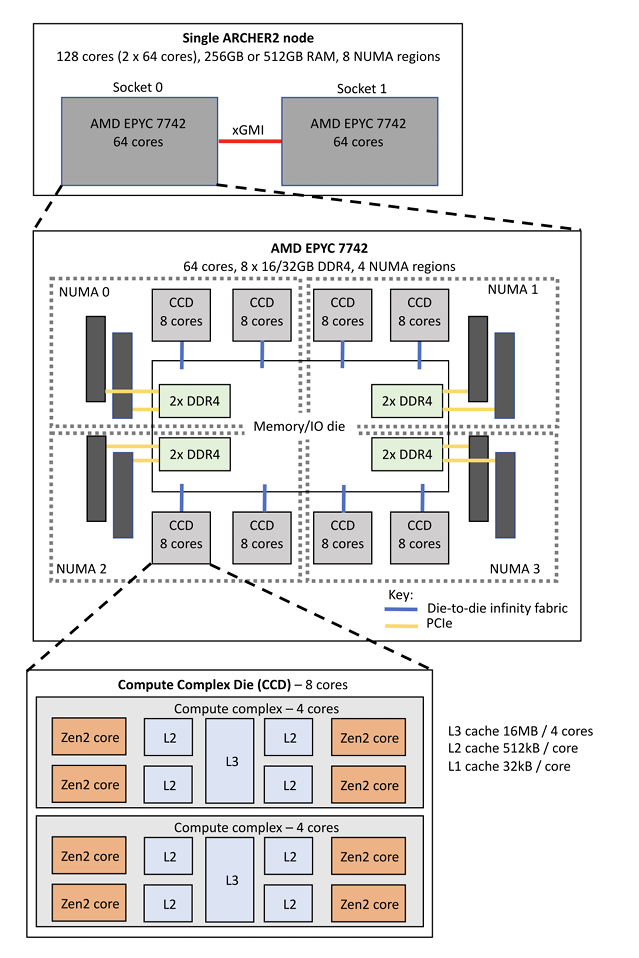
\includegraphics[width=0.58\textwidth]{archer2.png}
  \caption{Hierarchy of an ARCHER2 compute node. Each node has two 64-core AMD EPYC
  7742 processors, eight 16-core NUMA regions, and four-core CCXs that each share
  16\,MB of L3 cache. Source: ARCHER2 hardware documentation
  \cite{archer2_hardware}.}
  \label{fig:archer2_architecture}
\end{figure}

NUMA affects both latency and bandwidth. Linux normally places a page of memory in the NUMA
region of whichever thread writes to it first. If one thread initialises a large array and a
whole team reads it later from several regions, all that traffic falls on the memory
controllers of the one region that owns the pages. The ARCHER2 tuning guide also notes that
two threads can already come close to the memory-bandwidth limit of a NUMA region for
bandwidth-intensive code \cite{archer2_tuning}. More threads do not guarantee more
bandwidth.

The cache hierarchy draws a finer boundary than NUMA does: four adjacent cores share an L3
cache, and a 16-core NUMA region holds four such groups. Under the close binding of
\Cref{sec:placement}, the four full-node layouts therefore sit differently against that
boundary, as \Cref{tab:layouts} sets out.

\begin{table}[htbp]
  \centering
  \caption{Four fully populated layouts under close binding. All use 128 physical cores.
  What changes is the rank count and where a rank sits relative to the shared-L3
  boundaries. The table describes placement, not its performance effect.}
  \label{tab:layouts}
  \begin{tabular}{lrrl}
    \toprule
    Layout & Cores/rank & Subdomains/node & Rank against the shared-L3 (CCX) boundary \\
    \midrule
    $128\times1$ & 1 & 128 & four ranks share one CCX \\
    $64\times2$  & 2 &  64 & two ranks share one CCX \\
    $32\times4$  & 4 &  32 & exactly one CCX \\
    $16\times8$  & 8 &  16 & spans two CCXs \\
    \bottomrule
  \end{tabular}
\end{table}

Eight threads span two four-core L3 groups but stay inside one 16-core NUMA region, and no
layout tested here puts a rank across two NUMA regions. So the layouts cannot differ because
one of them reaches across a NUMA boundary, since none of them does. That rules out one
explanation. It does not prove an L3 or OpenMP one. \Cref{sec:map-matrix} later shows where
the sampled threads wait, without establishing why.

\section{PETSc and Krylov Solvers}
\label{sec:petsc-krylov}
PETSc provides distributed vectors and matrices, Krylov subspace solvers (KSP),
preconditioners (PC), and the logging infrastructure used in this study. PETSc uses MPI
for its distributed-memory communication and lets users select solver components at run
time \cite{petsc_manual_324,petsc1997}. Being able to swap components at run time is useful
for experiments. It also means that a comparison of layouts says nothing unless the
numerical method is doing comparable work in every layout.

The production system is the finite-difference Laplacian, whose matrix is sparse,
symmetric, and positive definite. Conjugate gradients (CG) is designed for this class of
linear system \cite{hestenes1952cg}. At each iteration CG applies the matrix and the
preconditioner, updates vectors, and evaluates inner products. These operations expose two
different scaling limits, and the distinction runs through the whole dissertation: the
sparse matrix-vector product exchanges halo values with \emph{neighbouring} subdomains,
whereas inner products and residual norms require a reduction across \emph{all} ranks.
\Cref{tab:cg-ops} classifies the work of one CG step accordingly.

\begin{table}[htbp]
  \centering
  \caption{PETSc events and measured calls in one GAMG-preconditioned CG step. A step is
  one preconditioner application. CG performs one more step per solve than its reported
  iteration count, because it preconditions the initial residual.}
  \label{tab:cg-ops}
  \begin{tabular}{lllr}
    \toprule
    Operation & PETSc event & Communication & Calls/step \\
    \midrule
    Matrix-vector product   & \texttt{MatMult}          & neighbour &  28.9 \\
    Multigrid restriction   & \texttt{MatMultTranspose} & neighbour &   7.0 \\
    Multigrid prolongation  & \texttt{MatMultAdd}       & neighbour &   7.0 \\
    Level residual          & \texttt{MatResidual}      & neighbour &   7.0 \\
    \addlinespace
    Halo exchange, all of the above & \texttt{VecScatterBegin} & neighbour & 42.9 \\
    \addlinespace
    Inner products          & \texttt{VecTDot}          & global    &   2.0 \\
    Residual norm           & \texttt{VecNorm}          & global    &   1.0 \\
    Vector updates          & \texttt{VecAXPY}, \texttt{VecAYPX} & none & 44.7 \\
    \bottomrule
  \end{tabular}
\end{table}
% VERIFIED 2026-07-31 from analysis/data/nproc_2d_libsci/logs/repeated_fullnode/165m/
%   nodes16/logs/ex2_..._ppn128_t1_job14528993_rep1.log. RE-CHECKED 2026-08-05 against
%   evidence/sanitized_logs/phase3_2d_weak_165m_32n_64x2.log, which reproduces every count
%   in the table to the digit (MatMult 7144/247=28.9, MatMultTranspose and MatMultAdd and
%   MatResidual 1729/247=7.0, VecTDot 494/247=2.0, VecScatterBegin 10602/247=42.9).
%   CORRECTION to the 2026-07-31 note: 247 is NOT the iteration count. RepeatedSolves has
%   KSPSolve 19, and VecNorm and PCApply are both 247 = 19 x 13, which is one MORE per
%   solve than the 12 iterations the log itself reports on its "Norm of error ... iterations
%   12 solves 20" line, because CG evaluates and preconditions the initial residual before
%   the first update. So 247 is the number of CG steps (equivalently, preconditioner
%   applications) in the stage; the actual outer iteration count is 19 x 12 = 228. The
%   counts above are stage event counts divided by 247, and 247 is the correct divisor:
%   only it makes the multigrid events integral (dividing by 228 gives 7.58 and 2.17). The
%   same +1 structure holds in every log checked: 20.25M reports 10 iterations with VecNorm
%   209 = 19 x 11, and the 3D 20M log reports 6 with VecNorm 133 = 19 x 7.
%   ALSO CORRECTED: the hierarchy has seven COARSENING STEPS, not seven levels. The Main
%   Stage of the 165M log carries PCGAMG Gal l00-l06, that is seven level transitions and
%   eight levels, which is why MatMultTranspose, MatMultAdd and MatResidual are 7.0 each:
%   one restriction, one prolongation and one residual per transition. The 20.25M problem
%   has six (Gal l00-l05) and gives 6.0 for the same three events. MatMult exceeds one per
%   step because the smoother applies it on every level. Consistency check on the halo row:
%   VecScatterBegin 42.9 = 28.9 + 7.0 + 7.0, one exchange per neighbour matrix operation.

The multigrid hierarchy exchanges halos on every level, giving about 43 neighbour
exchanges against three global reductions per step. \Cref{sec:bottleneck} measures both
because they scale differently with rank count.

A preconditioner reshapes the system so that CG reaches the requested tolerance in fewer
iterations. Algebraic multigrid (AMG) builds a hierarchy of coarser problems directly from
the matrix. On each level, smoothing removes the rapidly varying part of the error, and
restriction, coarse-grid correction and prolongation deal with the smooth part, which a
local smoother would take many sweeps to remove \cite{stuben2001amg}. PETSc's GAMG (geometric-algebraic multigrid,
\texttt{PCGAMG}) supplies this hierarchy without requiring a geometric mesh description
\cite{petsc_manual_324}. The name is historical. No geometric information is given to it
here.

GAMG has a setup phase and an application phase. \texttt{PCSetUp} builds the aggregates,
transfer operators, and coarse matrices. Each subsequent \texttt{PCApply} traverses the
multigrid hierarchy during \texttt{KSPSolve}. A solver that reuses the hierarchy across
several systems with the same operator pays the setup once, so first-solve time and
repeated-solve time answer different performance questions.

The choice of preconditioner also decides whether the comparison is valid at all. Block
Jacobi builds one block per MPI rank, so changing the layout changes the preconditioner
itself, and the runs being compared are no longer solving the problem the same way. AMG
does not have that property. \Cref{sec:solver} measures the effect and settles the
comparison on GAMG.

\section{Performance Analysis Tools}
\label{sec:tools}
PETSc's \texttt{-log\_view} reports time, flop counts, messages, reductions and named
events for each logging stage \cite{petsc_manual_324}. Events such as \texttt{MatMult},
\texttt{VecScatterEnd}, \texttt{VecTDot}, \texttt{PCSetUp} and \texttt{PCApply} connect
solver operations to measured costs. The report covers every layout, including the
$128\times1$ baseline, and supplies the comparable quantities used across layouts.

Linaro MAP samples source-level call paths together with CPU, memory, vectorisation and MPI
metrics \cite{linaro_map_2504}. It can tell apart cores running PETSc, cores waiting in MPI,
and cores sitting inside the OpenMP runtime. Its instrumentation adds a large and uneven
overhead, so MAP is used only to interpret the profiled hybrid layouts, while
\texttt{-log\_view} supplies the timings compared across layouts. Profiled timings are never
mixed with uninstrumented scaling results.

\section{Summary and Research Gap}
\label{sec:gap}
Prior work reports hybrid benefits for communication-heavy ARCHER2 applications
\cite{judge2022mpiopenmp} and for a specialised PETSc matrix kernel
\cite{lange_petsc_hybrid}. It does not evaluate PETSc 3.24's current threaded-kernel
backend with CG+GAMG across matched 2D and 3D stencil problems, nor map its rank--thread
balance across both scaling regimes. The open question here is narrower than whether hybrid
programming can be fast. It is whether this backend cuts steady-state solve time when the
node is fully populated with 128 cores either way, which balance is best as the job grows,
and which measured events go with the difference. This study fixes total cores, solver and
convergence criteria while varying layout, problem size and node count, then links runtime
to \texttt{-log\_view} and MAP evidence.

% PLAIN-LANGUAGE PASS 2026-08-09, ch:background, third in the series after sec:rqs and
%   ch:conclusion. WORDING ONLY except the two items marked below. No citation, number or
%   scope statement was touched, and the tables and the G11 topology note are unchanged.
%   Nominalisations opened out into verbs: "process-level decomposition, message matching,
%   and per-rank library state" -> "one subdomain per process, the cost of matching each
%   message to its receiver, and a separate copy of the library's state in every rank";
%   "its boundary-to-interior ratio grows" -> "more of it is boundary and less of it is
%   interior"; "may replicate solver or preconditioner metadata" -> "state that each rank has
%   to keep its own copy of"; "indirect memory access and low arithmetic intensity" -> "it
%   jumps around memory and does little arithmetic per value fetched"; "the runtime must
%   create or wake thread teams, distribute work, and synchronise them" -> "create or wake
%   the threads, hand out the work, and make them wait for each other at the end"; "parked in
%   an OpenMP runtime path" -> "sitting inside the OpenMP runtime"; "isolates concurrency
%   cost once local work is held approximately still" -> "holds the local work roughly still,
%   so that what is left to measure is the cost of running more things at once".
%   The AMG paragraph named the error components by frequency ("high-frequency error",
%   "components that a local smoother removes slowly") without saying they are the two halves
%   of one split; it now says rapidly varying against smooth, which is the same claim and
%   readable without a multigrid course.
%   Four semicolons joining independent clauses became full stops.
% AMBIGUITY FIXED, and this one was worth catching: sec:hybrid's last paragraph opened
%   "Weak hybrid scaling can reflect ...", meaning scaling that is POOR. Two paragraphs
%   earlier sec:flatmpi defines weak scaling as a REGIME, and \Cref{ch:multinode} reports a
%   whole weak-scaling campaign, so the phrase reads as "hybrid scaling in the weak-scaling
%   regime" on first pass. Now "When a hybrid run scales badly". Do not restore "weak" as an
%   evaluative word anywhere in this document.
% CLARIFIED, consistent with ch3: sec:petsc-krylov said block Jacobi "changes the operator
%   when the layout changes". In PETSc usage the operator is the matrix A, which does not
%   change here; what changes is the preconditioner. \Cref{sec:solver} already puts it that
%   way twice ("every additional rank changes the preconditioner", "Block Jacobi also makes
%   the preconditioner a function of the rank decomposition"), and tab:iterations-rank is the
%   evidence: iteration count is fixed by rank count alone, 6700 down to 2825 across rank
%   counts and constant along every row of threads. Now "changing the layout changes the
%   preconditioner itself".

% DOCUMENT-WIDE SWEEP 2026-08-09, after the sec:rqs / ch:conclusion / ch:background passes.
%   Looked for the same four faults everywhere else. What it found and fixed:
%   (1) FIVE banned adjectives, all reintroduced since the 2026-08-03 pass that removed them:
%       "far more accurate than intended" (sec:superseded) -> "five orders of magnitude more
%       accurate", which is the measurable version: intended 1e-5 against an effective
%       2.4e-10 at 6400^2, both already in that paragraph. "separate more clearly"
%       (sec:weak-3d) -> "are easier to tell apart". "rises sharply at each doubling"
%       (sec:sync-breakeven) -> "rises at every doubling of the thread count", which also
%       says WHICH doubling, since that table's rows are layouts. "The obvious reason"
%       (sec:sync-limits) -> "The first candidate", which is what the paragraph then does,
%       test it and find it insufficient in 2D. "only the clearest case" -> "only the most
%       extreme case of it", the wording that section's own VERIFIED note already used.
%   (2) The ABSTRACT said "Each formal configuration has three runs; one warm-up builds the
%       GAMG hierarchy before 19 timed solves reuse it", which reads as one warm-up per
%       CONFIGURATION. It is one per RUN, as sec:conclusions and sec:benchmarks both state.
%       Now "every run performs one warm-up solve ... followed by 19 timed solves".
%   (3) "monotone" is now GLOSSED at its first prose use in sec:weak-2d, because ch:profiling
%       and ch:discussion were rewritten to say "improves at every step" and the abstract
%       followed. Ch4 keeps the term, since tab:cross-dimension has a row named for it.
%       "Turns upward" stays defined in tab:cross-dimension's caption and used in Ch4 only.
%   (4) 44 semicolons joining two independent clauses, split. The document had drifted to
%       3.42 per 1000 words against the house ceiling of 2, and is now at 0.20. KEPT: the
%       three-part recommendation in sec:conclusions and the halo/reduction event definition
%       in tab:sync-split's caption, both lists whose items contain commas. Two elliptical
%       ones ("flat MPI at eight nodes; 64x2 and 32x4 at 16") became commas, not full stops.
%   Metrics after the sweep, against the table in the dissertation-prose-style skill:
%   em dashes 0 (limit 0-1), semicolons 0.20/1000 (limit 2), -ly 0.96% (limit 1%),
%   median sentence 18 words (target 18-22), sentences over 45 words 15 of 757 (was 17).
%   NOT CHANGED, deliberately: the % VERIFIED and % CLOSED notes throughout. They are the
%   audit trail, not prose, and are exempt from the style rules.

% ===== FILE: chapters/ch3_methodology.tex =====
\chapter{Experimental Platform and Methodology}
\label{ch:methodology}
% Fuller material + Chinese notes: ../dissertation_prep/01_draft_ch3_methodology.md.

\section{Hardware and Software Environment}
\label{sec:env}
The node hierarchy relevant to placement is described in \Cref{sec:archer2}. All
experiments used physical cores with simultaneous multithreading disabled. The software
stack was PrgEnv-gnu 8.4.0, gcc 11.2.0, cray-mpich 8.1.27, and PETSc 3.24.4. The early
single-node exploration used \texttt{arch-omp-opt}. The validated repeated-solve campaigns
used \texttt{arch-omp-libsci-rome-opt}, configured with the threaded
\texttt{libsci\_gnu\_mp.so.5.0}. LibSci is HPE Cray's tuned implementation of the Basic
Linear Algebra Subprograms (BLAS) and LAPACK, the standard interfaces for dense
vector--vector, matrix--vector and matrix--matrix operations. The \texttt{\_mp} variant
threads those kernels with OpenMP. A sparse Krylov solve runs on PETSc's own kernels and
reaches dense BLAS only incidentally. The library is therefore a possible confound rather
than a source of speed: its threads would be drawn from the same per-rank thread count and
pinned to the same cores as PETSc's, and would appear in the same OpenMP runtime that
\Cref{sec:map-matrix} measures. That section reports how much of the solve it accounts for.
Both builds enabled PETSc's OpenMP kernels and used
\texttt{-O3}. One thread per rank in the OpenMP-enabled build is the flat-MPI baseline.
% TODO: expand from 01 §3.1 (Core Complex Dies, shared L3, 2.25 GHz base frequency) — but
%   see the two warnings on that file before copying anything out of it.
% G12 (VERIFIED 2026-07-16 from raw logs): DO NOT reinstate 01 §3.1's sentence about "a
%   reference MPI-only build ... (arch-mpi-opt) was used for the baseline comparison".
%   Confirmed false: all 24 logs in analysis/data/mpi_only/logs/ self-report `on a arch-omp-opt`, so
%   arch-mpi-opt was never actually run. scripts/petsc_configure_archer2.sh does define
%   such a build ("drop the two --with-openmp* lines"), so the recipe exists — but no
%   surviving results come from it. The present text is already correct: one thread per
%   rank in the OpenMP build IS the MPI-only baseline, and that is what \Cref{sec:sweep}
%   uses. (An actual arch-mpi-opt run remains an optional weekend experiment.)

\section{Benchmark Problems and Drivers}
\label{sec:benchmarks}
Both benchmarks solve the Poisson equation $-\nabla^2 u = f$ on a rectangular domain with
homogeneous Dirichlet boundary conditions, discretised by second-order central finite
differences on a uniform grid. The unknowns are the interior grid points, so a row at the
edge of the grid omits the neighbours that fall outside it, and the mesh spacing is absorbed
into the right-hand side.

The 2D benchmark is based on PETSc's KSP tutorial \texttt{ex2}
(\texttt{src/ksp/ksp/tutorials/ex2.c} in the PETSc source tree \cite{petsc_ksp_ex2}). On an
$m \times n$ grid it assembles the five-point stencil, diagonal $4$ and off-diagonals $-1$,
into an $mn \times mn$ sparse matrix with five nonzeros per row. The 3D benchmark,
\texttt{3d\_repeat}, is a driver written for this project. It assembles the seven-point
stencil on an $m \times n \times p$ grid, with seven nonzeros per row and otherwise the same
structure. Both matrices are symmetric positive definite, and both drivers set
\texttt{MAT\_SYMMETRIC}.

It was added because the fraction of a subdomain's rows that couple off-rank differs between
the two dimensionalities, and the decomposition is what decides by how much. Both drivers
number the grid lexicographically, $Ii = i + jm + kmn$, and both give \texttt{MatSetSizes}
\texttt{PETSC\_DECIDE} for the local sizes. PETSc hands each rank a contiguous block of rows,
so a subdomain is a slab of that numbering and not a cube (\Cref{fig:decomposition}). Write
$L$ for the rows a rank owns. A row couples off-rank through $\pm 1$, $\pm m$ and, in 3D,
$\pm mn$, and the $\pm 1$ term crosses a rank boundary for at most two rows, so the halo a
rank exchanges is about
\[
  2\min(L,\,m) \quad \text{in 2D}, \qquad 2\min(L,\,mn) + 2\min(L,\,m) \quad \text{in 3D}.
\]
In 2D the $\pm m$ term is capped at $2m$, that is $2\sqrt{N}$, and stays small beside $L$. In
3D it is capped at $2mn$, and once $L$ falls below $mn$ every row has both its $k$ neighbours
off-rank, so the halo reaches $2L$ and cannot improve further. The 3D problem is therefore
not a harder stencil so much as a decomposition that runs out of interior much sooner.
\Cref{sec:threats} sets out what this scopes the results to.

\begin{figure}[htbp]
  \centering
  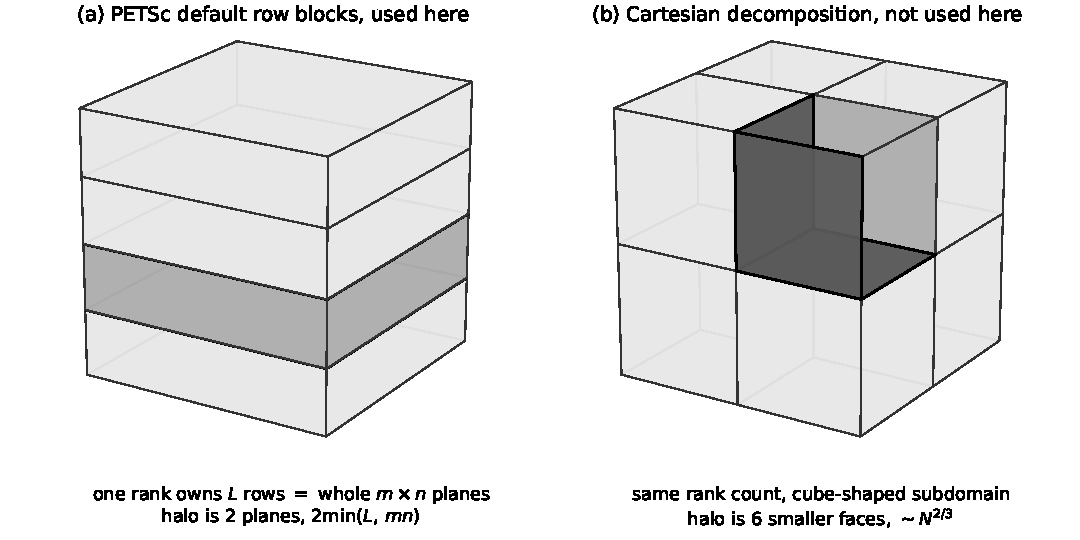
\includegraphics[width=0.92\textwidth]{decomposition_slab_vs_cube}
  \caption{How PETSc's default row blocks shape a subdomain. Contiguous rows of the
  lexicographic numbering make each rank's subdomain a stack of complete $m\times n$ planes,
  so the halo is the two planes it shares with its neighbours in $k$ and cannot fall below
  $2L$ once $L$ drops under $mn$. A Cartesian decomposition would cut the domain in every
  direction instead, giving six smaller faces. Every run in this dissertation uses (a); (b)
  is the alternative \Cref{sec:futurework} proposes. The shaded block is one rank's
  subdomain and the dark surfaces are what it exchanges.}
  \label{fig:decomposition}
\end{figure}

% MERGED 2026-08-09 with Leyan's original draft of this section, on request, and shortened.
%   RESTORED from the original, all three things the intervening rewrite had lost:
%   (a) the exact provenance of the 2D driver, "PETSc's KSP tutorial ex2
%       (src/ksp/ksp/tutorials/ex2.c in the PETSc source tree)" with a citation. The key
%       petsc_ksp_ex2 did NOT exist in references.bib and has been added as a @misc entry
%       pointing at the 3.24 source listing; biber resolves it and draft.bbl carries it.
%   (b) the REASON the 3D driver exists, which the rewrite had left implicit.
%   (c) the closing line "Everything timed in Ch4 is a steady-state solve in that sense",
%       and the naming of ex2_repeat and 3d_repeat as the two drivers, which the rewrite had
%       flattened to "both production drivers".
%   ONE THING NOT RESTORED, deliberately, and it is the reason this note exists. The original
%   gave the motivation as "the SURFACE-TO-VOLUME RATIO of a subdomain, and hence the
%   fraction of its rows that couple off-rank, differs between the two dimensionalities".
%   The conclusion is right and is kept; the mechanism is the one the 2026-08-08 correction
%   below refuted. Surface-to-volume is the CARTESIAN picture, and PETSC_DECIDE gives slabs,
%   not cubes: a 3D subdomain's halo is two whole m x n planes and saturates at 2L, which is
%   not a surface-to-volume statement about a cube. The sentence now reads "the fraction of a
%   subdomain's rows that couple off-rank differs between the two dimensionalities, and the
%   decomposition is what decides by how much", which keeps the original's claim and hands
%   the mechanism to the halo model in the same paragraph. Do not restore the original
%   wording without also reopening the 2026-08-08 correction.
%   Shortened elsewhere: the discretisation paragraph lost "The unknowns are the interior
%   grid points, so the boundary values never enter the linear system" (the clause after it
%   says the same thing operationally) and "which leaves the standard stencil coefficients";
%   the 3D stencil lost "diagonal 6 and off-diagonals -1", which the original never carried
%   and which "seven-point stencil" implies; "so that PETSc may exploit it" after
%   MAT_SYMMETRIC; the known-solution and grid-matching paragraphs merged into one; the six
%   grid extents replaced by "six sizes from 5.0M to 164.6M in each dimension", since
%   tab:fullnode-matrix lists every one of them two pages later and the sentence already
%   points at it. No number, formula, cross-reference or scope statement was dropped.
% VERIFIED 2026-08-08. CORRECTION, raised by Leyan from the source. The paragraph above
%   REPLACES a justification that was factually wrong about this code: "A subdomain of N
%   unknowns has a boundary that grows as N^(1/2) in 2D and as N^(2/3) in 3D". That is the
%   textbook formula for CARTESIAN subdomains, and these drivers do not produce them.
%   src/3d_repeat.c and src/ex2_repeat.c both call MatCreate + MatSetSizes(PETSC_DECIDE,
%   PETSC_DECIDE, N, N) and index lexicographically (3d_repeat.c lines 37-38 and 46-48).
%   There is no DMDA, no MatSetLocalToGlobalMapping and no custom partitioner anywhere in
%   src/ -- checked all four .c files. PETSC_DECIDE routes to PetscSplitOwnership, which
%   gives contiguous row ranges, so a subdomain is a SLAB of the lexicographic numbering.
%   The replacement model, halo ~ 2min(L,mn) + 2min(L,m), was checked against the measured
%   neighbour_pct in repeated_fullnode_event_matrix.csv at all 48 points of the ~40k chains
%   (2 dimensions x 6 size-node points x 4 layouts):
%     3D flat MPI along the chain: predicted halo/L 1.51, 2.01, 2.01, 2.02, 2.02, 2.03
%       against measured neighbour_pct 35.1, 47.6, 50.1, 53.7, 59.1, 70.9 -- both monotone,
%       and the prediction SATURATES at 2.0 exactly where the measured share flattens.
%     2D flat MPI: predicted 0.11 -> 0.64, measured 15.9% -> 34.3%.
%     Layout ORDERING at a fixed size-node point: predicted correctly at 48 of 48. Hybrid
%       owns 2/4/8x more rows, so its ratio is 2/4/8x smaller, which is the measured order.
%   CAUTION, and the reason the text says "predicts" and not "explains": the model is a
%   VOLUME model and neighbour_pct is a TIME share. At 3D 165m/32n the four predicted
%   ratios are nearly equal (2.03, 2.01, 2.01, 1.87) while the measured shares span 17.7
%   points (70.9, 59.0, 54.8, 53.2), so volume alone does not carry the layout ordering
%   there -- message count and per-rank metadata must. That is consistent with
%   sec:sync-limits, which already states that the exposure share cannot separate them.
%   Do not upgrade this to a fitted or causal claim without that separation.
%   Cube-subdomain comparison quoted in sec:threats: at 164.56M on 32 nodes, L = 40177, so
%   a cube edge is 40177^(1/3) = 34.25 and the halo is 6*34.25^2 = 7038, i.e. 0.18L against
%   the actual 2.03L; in 2D a square edge is 200.4, halo 4*200.4 = 802, i.e. 0.02L against
%   the actual 0.64L. Grid edges recovered from unknowns_per_core * cores and confirmed
%   integral: 3D 171/215/273/345/435/548 cubed, 2D 2240/3160/4500/6400/9073/12828 squared.
%   NO MEASURED NUMBER CHANGES. Every timing, exposure share, ratio and fit in the thesis
%   stands: all layouts run the same code under the same decomposition, so the layout
%   comparison is unaffected. What changed is the ATTRIBUTION, here and at sec:sync-halo,
%   plus new scope text in sec:threats, sec:futurework and sec:rq4.

Neither problem uses an analytic forcing term. Both set the exact solution to
$u=\mathbf{1}$ and form $b=Au$, so every run reports $\lVert x-u\rVert_2$ as an end-to-end
known-solution check that makes a silently wrong solve visible in the log. The grids are
matched in unknowns rather than in grid extent: six sizes from 5.0M to 164.6M in each
dimension, each 2D size paired with a 3D one to within 0.5\%. \Cref{tab:fullnode-matrix}
lists them with the node counts at which each was run.

Both benchmarks are run through a repeated-solve driver rather than solved once.
\texttt{ex2\_repeat} separates one warm-up \texttt{KSPSolve} from 19 timed solves inside a
dedicated \texttt{RepeatedSolves} logging stage, with the operator and preconditioner
unchanged across the timed solves, and \texttt{3d\_repeat} applies the same design in 3D. The
initial guess is zeroed before each timed solve, or the previous solution would already
satisfy the tolerance and the next solve would return at iteration zero.
\Cref{sec:whyrepeat} gives the reason and the measured cost split that motivates it.
Everything timed in \Cref{ch:multinode} is a steady-state solve in that sense.

\section{Solver Configuration}
\label{sec:solver}
The default \texttt{ex2} solver is GMRES with one block-Jacobi block per MPI rank and an
ICC factorisation inside each block. A serial run therefore factors the whole matrix,
whereas every additional rank changes the preconditioner. At $2240\times2240$ and above,
every run reached PETSc's 10,000-iteration limit with \texttt{DIVERGED\_ITS}. Final error
norms were of order $10^0$--$10^3$. The jobs also used an unintended mesh-dependent
tolerance, as \Cref{sec:superseded} establishes, so the observed non-convergence is a
joint effect and does not isolate either cause.

Production runs use
% VERIFIED 2026-07-16 against the raw logs in analysis/data/size_grid/logs/*/ (the derived CSVs are
%   gone): 213 logs, 4 empty (failed jobs), 149 of the 209 with results end in
%   "Linear solve did not converge due to DIVERGED_ITS iterations 10000".
% CORRECTED 2026-07-31: the earlier note inferred "KSPGMRESOrthog => GMRES". That
%   inference is unsound — KSPGMRESOrthog appears in 100% of logs in EVERY campaign,
%   including runs confirmed to use CG, because GAMG's setup uses GMRES internally for
%   eigenvalue estimation. The discriminating evidence is MatICCFactorSym (209/209 in
%   size_grid, 0 in every GAMG campaign) for the block-Jacobi+ICC sub-solver, and a
%   stage-scoped read of RepeatedSolves (VecTDot = 2 x VecNorm, no VecMDot) for CG.
%   PCSetUpOnBlocks/PCApplyOnBlocks is likewise NOT discriminating; it appears in the
%   GAMG runs too. Norm range per scale: small
%   0.011-0.016 (converged), medium-small 7.2-65, medium 62-553, large 768-1762,
%   very-large 2109-3768. The old "order 10^10" claim came from the deleted CSVs'
%   unparseable error_norm column and is refuted by the logs.
\begin{verbatim}
-ksp_type cg -pc_type gamg -ksp_rtol 1e-5 -ksp_atol 1e-10
\end{verbatim}
CG applies because the discretised Laplacian is symmetric positive definite. GAMG is used
because multigrid convergence is close to mesh-independent for elliptic problems. Across
5.0M to 164.6M unknowns, the final solve takes 9--13 iterations in 2D and 6--7 in 3D.
Observed error norms range from $8.5\times10^{-3}$ to $1.34\times10^{-1}$ in 2D and from
$6.0\times10^{-3}$ to $8.59\times10^{-2}$ in 3D. Small layout-dependent changes in
iteration count affect close throughput comparisons, so the results report both equations
solved per second and time per KSP iteration.
% FIXED 2026-07-16: was "11--12 iterations". Real range from ksp_2d_aggregated.csv is
%   10--13, and it grows mildly with size (small 10-11, medium 10-11, large 11-12,
%   very-large 12-13) — hence "near-constant" / "close to mesh-independent", not "constant".

Block Jacobi also makes the preconditioner a function of the rank decomposition.
\Cref{tab:iterations-rank} shows the consequence: iteration count is constant across
threads at a fixed rank count but varies by more than a factor of three across rank counts.

\begin{table}[htbp]
  \centering
  \caption{Final iteration count of the single-node default-solver sweep on a
  $1000\times1000$ grid, for every $\text{ranks}\times\text{threads}\leq128$ combination.
  Every row is constant: the count is fixed by the rank count alone. The 128-rank
  configuration reached the 10,000-iteration limit without converging.}
  \label{tab:iterations-rank}
  \begin{tabular}{lrrrrrrrr}
    \toprule
    & \multicolumn{8}{c}{OpenMP threads per rank} \\
    \cmidrule(lr){2-9}
    MPI ranks & 1 & 2 & 4 & 8 & 16 & 32 & 64 & 128 \\
    \midrule
    1   &  6700 & 6700 & 6700 & 6700 & 6700 & 6700 & 6700 & 6700 \\
    2   &  3715 & 3715 & 3715 & 3715 & 3715 & 3715 & 3715 &      \\
    4   &  2825 & 2825 & 2825 & 2825 & 2825 & 2825 &      &      \\
    8   &  4085 & 4085 & 4085 & 4085 & 4085 &      &      &      \\
    16  &  8179 & 8179 & 8179 & 8179 &      &      &      &      \\
    32  &  6460 & 6460 & 6460 &      &      &      &      &      \\
    64  &  7181 & 7181 &      &      &      &      &      &      \\
    128 & 10000 &      &      &      &      &      &      &      \\
    \bottomrule
  \end{tabular}
\end{table}
% VERIFIED 2026-07-31 by analysis/scripts/size_grid/analyze_single_node_sweep.py, which
%   parses all 62 non-empty logs in analysis/data/size_grid/logs/small/ and RAISES if the
%   iteration count is not constant across thread counts at any fixed rank count. It also
%   rejects any log whose header arch is not arch-omp-opt, that carries PCGAMG events, or
%   that lacks MatICCFactorSym. Table CSV: data/size_grid/tables/iterations_vs_layout.csv.

The series repeats exactly across repetitions and is non-monotonic in rank count. Reading
across a row changes the thread count but not convergence. Reading down a column changes
the block decomposition and the iteration count by more than a factor of three. Layouts
with different rank counts therefore apply different preconditioners to the same system,
so their wall-clock times cannot answer which rank--thread layout is fastest.

GAMG removes the direct one-block-per-rank coupling. At a fixed size and node count,
layouts differ by at most two iterations in 2D and one in 3D, rather than by thousands.
Reporting time per outer KSP iteration takes that convergence variation out, although it
does not make GAMG hierarchy work or communication identical across decompositions. Results therefore
report both raw throughput and time per iteration.
% Merged here 2026-07-16 from the deleted §4.3 "Effect of Solver Choice". Evidence
%   RE-VERIFIED 2026-07-16 from raw logs (the CSVs are deleted): the "Linear solve" line
%   in analysis/data/size_grid/logs/small/*.log gives the series above, identical across every thread
%   count and both jobids (13996330/13997004). Cross-campaign check at 800²:
%   analysis/data/mpi_only/logs/ (Feb, job12590513) and analysis/data/fixed128_multinode/logs/ nodes1 (Jul) give
%   identical counts for r16/32/64/128 = 5052/4173/5150/6567. Multi-NODE placement shifts
%   counts <1% (r128: 6567 on 1 node, 6571/6615 on 2/4 nodes — FP reduction order), which
%   does not affect the argument. GAMG side: analysis/data/ksp_2d_scaling/csv/derived/
%   ksp_2d_aggregated.csv `iterations_median`, range 10-13 incl. multi-node rows.
% DONE 2026-07-31: the eight-number series is now \Cref{tab:iterations-rank}.

GAMG's two phases carry very different costs, so the production campaign times repeated
solves with the hierarchy reused rather than first solves. \Cref{sec:whyrepeat} gives the
measured split and the driver that produces it. A fuller default-versus-GAMG table would
require additional matched converged points and is not used for the layout claims in this
dissertation.

\section{Configuration Space and Selection Rules}
\label{sec:configspace}
Three rules define the formal configuration space. Threads per rank are restricted to
$\{1,2,4,8\}$ because 16 or more cost substantially more per iteration in both the
exploratory and production configurations (\Cref{sec:sweep}). This is an empirical search
bound, not a NUMA or cache claim.

Nodes are fully populated: $\text{ppn} \times \text{threads} = 128$, giving four layouts
$128\times1$, $64\times2$, $32\times4$, and $16\times8$. Same node count means same core
count, so a comparison isolates rank--thread balance from core count.

A configuration at size $N$ on $C$ physical cores is included when
$25{,}000 \leq N/C \leq 100{,}000$. The completed 2D campaign uses six grids:
$2240^2$, $3160^2$, $4500^2$, $6400^2$, $9073^2$, and $12828^2$, or 5.02M to
164.56M unknowns. The filter admits 11 size--node pairs over 1--32 nodes. Each admitted
pair runs all four layouts and three formal repeats.

\section{Bounding the Thread Count}
\label{sec:sweep}
The first rule of \Cref{sec:configspace} is the only one that had to be measured rather
than chosen, and it rests on two campaigns with complementary weaknesses. The exploratory
sweep below covers every rank--thread combination on one node, but runs the default solver,
whose preconditioner changes with the rank count. The production campaign that follows it
runs exactly the solver, build and driver of \Cref{ch:multinode} at two, four and eight
nodes, but only one repeat per configuration. Both give the same answer, and the
restriction is applied only because they agree.

\subsection{Exploratory Single-Node Sweep}
\label{sec:sweep-exploratory}
% G2 RESOLVED 2026-07-16: re-derived from the raw logs in analysis/data/size_grid/logs/small/ (1M,
%   jobs 13996330/13997004). Both survivors verified per-iteration:
%     - pure OpenMP fails: 1 rank is 6700 iterations at every thread count;
%       245.7 s (t1) -> 208.4 s (t128), best 195.6 s at t64. Clean like-for-like. KEPT.
%     - >=16 threads per rank is worse: at 128 cores, KSPSolve ms/iteration is
%       0.38 (128x1), 0.60 (64x2), 0.98 (32x4), 1.88 (16x8), 3.65 (8x16) ... 31.05
%       (1x128) — a monotone trend in rank count, not a threshold at 16. KEPT.
%   The restriction is argued from per-iteration cost in §3.5. Honest framing stands: a
%   pragmatic bound from the default-solver sweep. Corrected CG+GAMG production data in
%   Ch4 favour 64x2 per iteration. Do not claim the sweep proves hybrid benefit.
% G11 CLOSED 2026-08-01: the measured topology is now in \Cref{sec:archer2}. Note that
%   16 threads per rank exactly FILLS one 16-core NUMA region rather than spanning two,
%   so the restriction is argued from per-iteration cost, never from a NUMA mechanism.

The sweep ran every rank--thread combination with
$\text{ranks} \times \text{threads} \le 128$ on a $1000 \times 1000$ grid (one million
unknowns). It predates the solver change, so it uses the default configuration and, by the
argument of \Cref{sec:solver}, it cannot rank layouts with different rank counts. It can
still bound the configuration space, because the conclusions drawn from it hold at a fixed
rank count, where the preconditioner is also fixed. Every run reported here comes from the
same build and the same campaign, and the two extremes below share one baseline: a single
rank on a single thread, $245.7\,\text{s}$ at 6700 iterations.

\Cref{fig:single-node-sweep} contrasts the two ways of using the node's 128 cores, both
measured from that shared baseline. Both lines are normalised per KSP iteration, which is
what makes them comparable: the threads-only line holds the preconditioner fixed by
construction, while the ranks-only line changes it at every point, and its 128-rank
configuration never converged.

\begin{figure}[htbp]
  \centering
  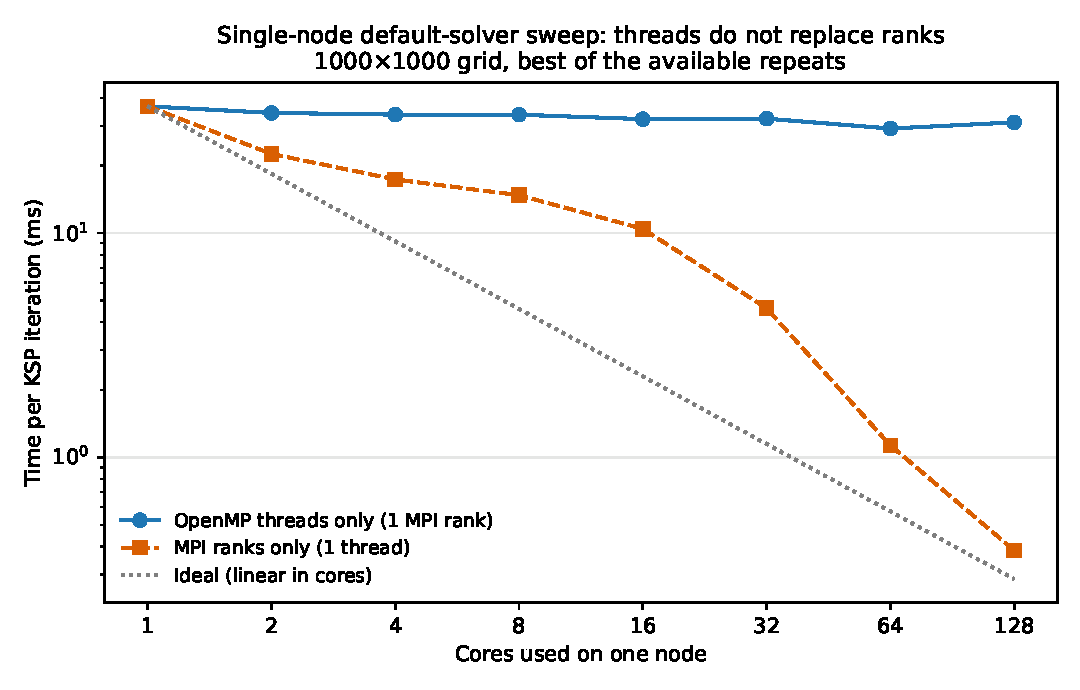
\includegraphics[width=0.85\textwidth]{size_grid_single_node_cost_per_iteration}
  \caption{Single-node default-solver sweep on a $1000\times1000$ grid. Adding OpenMP
  threads to one MPI rank leaves the cost per iteration almost unchanged. Adding MPI ranks
  at one thread each reduces it by two orders of magnitude. Both lines start from the same
  one-rank, one-thread run.}
  \label{fig:single-node-sweep}
\end{figure}

Pure OpenMP does not scale. A single rank takes 6700 iterations at every thread count, so
these runtimes are directly comparable, and they barely move: $245.7\,\text{s}$ at one
thread, $225.5$ at eight, $216.5$ at thirty-two, $195.6$ at sixty-four, and $208.4$ at
128. The best case is a factor of 1.26 at 64 threads, after which more threads cost time
again. At 128 threads the return is a factor of 1.18 for 128 times the cores. Over the whole
threads-only line the cost per iteration spans a factor of 1.26. Over the ranks-only line
it spans 95.4. The OpenMP backend parallelises only part of the execution path, and the
serial remainder bounds the achievable speedup. \Cref{ch:profiling} returns to this with
profiler evidence.

The MPI-only line from the same baseline reaches $8.1\,\text{s}$ on 64 ranks, a factor of
30. Its rank counts differ, so by \Cref{sec:solver} the wall-clock figure is indicative
rather than a measurement of parallel efficiency. The 64-rank run performs \emph{more}
iterations than the baseline (7181 against 6700), so iteration count cannot account for
any of the gap. Distributing this problem across the node works, and threading it does not.

Cost per iteration also falls monotonically as ranks replace threads at a fixed core
count, as \Cref{tab:fullnode-cost} shows: the trend is in the rank count, with no
threshold at any particular thread count.

\begin{table}[htbp]
  \centering
  \caption{Cost per KSP iteration for the eight fully populated single-node layouts
  ($\text{ranks}\times\text{threads}=128$) on a $1000\times1000$ grid. The trend is
  monotone in the rank count, with no threshold at any particular thread count. The
  $128\times1$ figure is measured over its non-converged 10,000 iterations, which still
  gives a valid per-iteration cost.}
  \label{tab:fullnode-cost}
  \begin{tabular}{lrrrl}
    \toprule
    Layout & Iterations & Repeats & ms per iteration & Converged \\
    \midrule
    $1\times128$ &  6700 & 1 & 31.10 & yes \\
    $2\times64$  &  3715 & 1 & 14.42 & yes \\
    $4\times32$  &  2825 & 1 &  7.24 & yes \\
    $8\times16$  &  4085 & 1 &  3.67 & yes \\
    $16\times8$  &  8179 & 2 &  1.89 & yes \\
    $32\times4$  &  6460 & 2 &  0.99 & yes \\
    $64\times2$  &  7181 & 2 &  0.61 & yes \\
    $128\times1$ & 10000 & 2 &  0.39 & no \\
    \bottomrule
  \end{tabular}
\end{table}
% VERIFIED 2026-07-31 by analysis/scripts/size_grid/analyze_single_node_sweep.py from the
%   raw logs. Where two repeats exist the values agree to the quoted precision
%   (16x8 1.888-1.893, 32x4 0.9898-0.9910, 64x2 0.6084-0.6092, 128x1 0.3844-0.3866).
%   Table CSV: analysis/data/size_grid/tables/fullnode_cost_per_iteration.csv.
%   NOTE: these are rounded from ms/iteration = Time(sec)/iterations, so they differ in the
%   second decimal from the pre-2026-07-31 prose (14.36/7.20/3.65/1.88/0.98/0.60/0.38),
%   which was read off KSPSolve rather than total Time(sec). Total time is used here for
%   consistency with the wall-clock figures quoted earlier in this section.
% Merged here 2026-07-16 from the dissolved Ch4 "Single-Node Performance Evaluation".
%   Only the per-iteration-safe findings survived; the wall-clock claim that 2-4 threads
%   beat MPI-only was an artefact of block Jacobi block count (see §3.3) and is gone,
%   along with §4.3 "Effect of Solver Choice".
% SOURCE (changed again 2026-07-16, evening): all numbers now come from
%   analysis/data/size_grid/logs/small/*.log (1000x1000 = 1M, arch-omp-opt, jobs 13996330/13997004),
%   because runs/rank_thread_grid/ (the 800² source used briefly) has been DELETED.
%   Same virtues hold: one build, one campaign, and the pure-OpenMP and MPI-only lines
%   share the identical 1-rank/1-thread baseline (245.7 s, 6700 it). Extract from the
%   "Linear solve"/"Time (sec):"/KSPSolve lines in each log. Combos with t<=8 have two
%   reps (both jobids); t>=16 combos have one. Numbers above are from job13996330 rep1.
%   DO NOT pull the MPI-only line from analysis/data/mpi_only/logs/ instead — see G12 below.
% NOTE the honest framing already in the text: this sweep BOUNDS the space, it does not
%   answer which layout is fastest. That question is answered in \Cref{ch:multinode} on
%   CG+GAMG data. Do not let the two get conflated when writing.
% G12 RESOLVED 2026-07-16 (verified from raw logs): analysis/data/mpi_only/logs/ is NOT a separate
%   MPI-only build — all 24 logs are named `arch-mpi-opt` but self-report
%   `on a arch-omp-opt` (label is the job script's, not the binary's). The 1.53x anomaly
%   STANDS, reconstructed indirectly since its direct baseline (rank_thread_grid) is
%   deleted: scaling the size_grid 1M serial run by iteration and size ratios predicts
%   245.7 x (4311/6700) x 0.64 = 101.2 s at 800², matching the deleted 101.3 s baseline;
%   mpi_only measures 154.7 s = 1.53x slower per unit work. Direct same-config check:
%   r128_t1 KSPSolve 2.076 s (mpi_only) vs 1.659 s (fixed128_multinode nodes1) = 1.25x.
%   So the Feb campaign is systematically 1.25-1.5x slower than newer equivalents; cause
%   still unknown (candidates: CPU frequency 3.4/2.25 = 1.51; unbound memory on a remote
%   NUMA node). RULE (relaxed): within-campaign relatives are fine (iteration counts match
%   fixed128_multinode exactly); absolute times need a caveat; cross-campaign absolute
%   comparisons remain off-limits.
% G11 CLOSED, but the MECHANISM for the per-iteration trend is still open. The topology is
%   now measured (\Cref{sec:archer2}) and \Cref{sec:map-matrix} names OpenMP wait time as
%   the cost that grows with threads/rank — but that is a software observation on a
%   different (CG+GAMG, LibSci) campaign. Do NOT retrofit it to this default-solver sweep,
%   and do not assert a NUMA or cache mechanism for either.
% G9 DONE 2026-07-31: \Cref{fig:single-node-sweep}. Both lines are per-iteration rather
%   than speedup, so the MPI-only line's varying iteration count cannot distort it.
% G7 (this section): repetition counts stated in SOURCE note above; when a number goes in
%   the text, cite it as one run or give both reps' spread (e.g. 4x4 ms/it is 9.6-12.0).

\subsection{The Same Bound on the Production Configuration}
\label{sec:sweep-production}
The sweep above cannot rank layouts with different rank counts, so the restriction was
re-tested on the production configuration before it was applied to the formal campaigns. A
separate multi-node campaign ran the same \texttt{arch-omp-libsci-rome-opt} build, the same
\texttt{ex2\_repeat} driver, and the same CG+GAMG options as \Cref{ch:multinode}, at 2, 4
and 8 nodes, and included the two layouts this rule excludes: $8\times16$ and $4\times32$.
\Cref{tab:thread-limit} gives the result. In all nine size--node cells the time per
iteration increases monotonically with threads per rank, and the excluded layouts are not
marginal: $8\times16$ costs $1.8$--$3.8$ times the best layout in its cell and $4\times32$
costs $3.0$--$7.4$ times. The rule therefore separates factor-level penalties from the
few-per-cent differences among the admitted layouts.

\begin{table}[htbp]
  \centering
  \caption{KSP time per iteration for five full-node layouts in the production
  configuration. Each cell has one run and every row rises with threads per rank. The
  campaign has no $128\times1$ cell and bounds the search space rather than ranking the
  admitted layouts.}
  \label{tab:thread-limit}
  \begin{tabular}{lrrrrrrrl}
    \toprule
    & & & \multicolumn{5}{c}{ms per KSP iteration} & \\
    \cmidrule(lr){4-8}
    Scale & Nodes & Unknowns/core & $64\times2$ & $32\times4$ & $16\times8$ & $8\times16$ & $4\times32$ & Iterations \\
    \midrule
    2m  & 2 &  7,810 &  1.75 &  2.25 &  3.52 &  6.08 & 11.82 & 9 \\
    2m  & 4 &  3,905 &  1.41 &  1.49 &  2.27 &  3.50 &  6.34 & 8--9 \\
    2m  & 8 &  1,953 &  1.30 &  1.30 &  1.64 &  2.32 &  3.88 & 8--9 \\
    \addlinespace
    4m  & 2 & 15,625 &  3.17 &  4.06 &  6.79 & 12.06 & 23.60 & 9--10 \\
    4m  & 4 &  7,813 &  2.13 &  2.52 &  3.80 &  6.46 & 12.39 & 8--9 \\
    4m  & 8 &  3,906 &  1.78 &  1.90 &  2.45 &  3.79 &  7.56 & 8--9 \\
    \addlinespace
    10m & 2 & 39,006 & 11.79 & 13.25 & 20.01 & 30.68 & 61.51 & 9--10 \\
    10m & 4 & 19,503 &  4.56 &  5.61 &  9.00 & 15.59 & 30.70 & 9--10 \\
    10m & 8 &  9,752 &  3.10 &  3.28 &  5.05 &  8.65 & 17.03 & 9--10 \\
    \bottomrule
  \end{tabular}
\end{table}
% VERIFIED 2026-08-03 by analysis/scripts/nproc_2d_libsci/analyze_multinode_thread_limit.py,
%   which parses all 45 raw logs under analysis/data/nproc_2d_libsci/logs/multi_node/ with
%   the formal campaign's content checks (reported arch, MPI process and OpenMP thread
%   counts, 20 converged solves, 19 timed KSPSolve events, no PCSetUp in the stage, the
%   configured LibSci path), reconciles all 45 against the independently retrieved job CSV
%   rows in csv/derived/fullnode_runs.csv, and RAISES unless ms/iteration is monotone in
%   threads per rank at every (scale, nodes) cell. Table CSV:
%   analysis/data/nproc_2d_libsci/tables/multinode_thread_limit.csv.
%   DISCRIMINATORS (per the provenance rules): all 45 logs report
%   `on a arch-omp-libsci-rome-opt`, carry PCGAMG events, carry no MatICCFactorSym, and
%   show the CG signature VecTDot = 2 x VecNorm inside RepeatedSolves. This is Phase 3
%   data, not the Phase-1 default-solver sweep.
%   LIMITS, stated in the caption: one run per cell, so no observed range; no 128x1 cell;
%   only the 10m/2-node row sits inside the 25k-100k unknowns/core window.

One run cannot resolve the 0.5\% difference between $64\times2$ and $32\times4$ at 2m on
eight nodes. The formal campaigns rank the admitted layouts. This campaign only excludes
16 and 32 threads per rank. The study therefore retains 1, 2, 4 and 8.

\section{Job Configuration and Thread Placement}
\label{sec:placement}
Each rank and its threads are pinned to a contiguous set of cores with:
\begin{verbatim}
OMP_PLACES=cores   OMP_PROC_BIND=close
srun --hint=nomultithread --distribution=block:block --exact
\end{verbatim}

Each setting is part of the layout definition. \texttt{OMP\_PLACES=cores} makes a place
one physical core and prevents migration. \texttt{OMP\_PROC\_BIND=close} places a rank's
threads on adjacent cores. \texttt{-{}-hint=nomultithread} selects 128 physical cores rather
than 256 SMT siblings. \texttt{-{}-distribution=block:block} assigns consecutive ranks to
consecutive cores, while \texttt{-{}-exact} restricts each task to its requested
\texttt{-{}-cpus-per-task} cores. Under the measured topology of \Cref{sec:archer2}, a
$32\times4$ rank occupies one four-core shared-L3 domain and a $16\times8$ rank occupies
two. No tested layout places a rank across two 16-core NUMA regions. Fixed pinning prevents
placement variation from obscuring the few-per-cent layout effects under study.

\section{Metrics}
\label{sec:metrics}
The primary timing is the maximum-rank \texttt{KSPSolve} time in the
\texttt{RepeatedSolves} stage. If this event has count $c=19$, time $t$, and the grid has
$N$ unknowns, steady-state throughput is
\[
  Q = \frac{Nc}{t}.
\]
The analysis also reports $t/(cI)$, where $I$ is the final KSP iteration count. Formal
repeats are aggregated by their median. Whiskers show the observed minimum and maximum
from three runs. Scaling is computed per layout against that layout's smallest admitted
node count. For a layout $\ell$ at $n$ nodes,
\[
  S_\ell(n) = \frac{T_\ell(n_0)}{T_\ell(n)}, \qquad
  E_\ell(n) = \frac{S_\ell(n)}{n/n_0},
\]
where $n_0$ is the smallest node count run for that problem size.

Two percentage conventions are kept distinct. For hybrid throughput $Q_h$ and flat-MPI
throughput $Q_m$, the throughput gain is $Q_h/Q_m-1$. For their times $t_h$ and $t_m$,
the time saving is $1-t_h/t_m$. They describe the same pair of runs but are not numerically
equal. Every percentage in the results names the convention it uses. Time per iteration is
used to separate convergence-count differences, not to claim identical multigrid work.
The three-run minimum and maximum describe only the variation observed in this campaign.
They are neither a confidence interval nor a significance test. When two observed ranges
overlap, the text treats the result as unresolved instead of selecting the smaller median.
When they do not overlap, the result supports a difference within this sample but still
does not establish a universal ordering beyond the tested configuration.
Every direct layout comparison also holds problem size, node count, total physical cores,
solver options and convergence tolerance fixed. Comparisons across scaling regimes remain
separate even when they share an anchor point.

\section{Superseded Campaigns}
\label{sec:superseded}
Two earlier campaigns were discarded before the formal study. Their defects are retained
here because neither was visible in the resulting plots, and each motivated a check now
enforced by the analysis pipeline.

The first round did not use its requested tolerance. All four drivers inherit a mesh-dependent relative
tolerance from upstream \texttt{ex2} before \texttt{KSPSetFromOptions} is called:
$\text{rtol} = 10^{-2}/((m+1)(n+1))$ in 2D and the corresponding product in 3D
(\texttt{src/ex2\_repeat.c:109} and siblings). The exploratory job script overrode it with
a double-dashed option, \texttt{-{}-ksp\_rtol 1e-5}, while neighbouring single-dashed
options took effect. Iterations rose by 39--62\% between the $800^2$ and $1000^2$
campaigns. The compute-node test in \Cref{tab:rtol} shows why.

\begin{table}[htbp]
  \centering
  \caption{Relative tolerance actually used by \texttt{ex2} on a $100\times100$ grid, read
  from \texttt{-ksp\_view}, for the three option styles. The double dash is silently
  ignored and the mesh-dependent default survives. \texttt{-options\_left} names the
  unconsumed option explicitly.}
  \label{tab:rtol}
  \begin{tabular}{llrl}
    \toprule
    Run & Option as passed & \texttt{relative=} & Iterations \\
    \midrule
    G13-a & \texttt{-{}-ksp\_rtol 1e-5} & $9.80\times10^{-7}$ & 84 \\
    G13-b & \texttt{-ksp\_rtol 1e-5}    & $1\times10^{-5}$    & 65 \\
    G13-c & none                        & $9.80\times10^{-7}$ & 84 \\
    \bottomrule
  \end{tabular}
\end{table}
% G13 CLOSED 2026-08-01 from scripts/ksp/diagnostics/petsc_diagnostics.14598711.out,
%   sections G13-a/b/c. G13-a is byte-identical to the no-override control G13-c
%   (relative=9.80296e-07 = 1e-2/(101*101), 84 iterations) and PETSc printed
%   "Option left: name:--ksp_rtol value: 1e-5 source: command line". The single-dash
%   control gives relative=1e-05 and 65 iterations. This confirms the indirect evidence
%   recorded on 2026-07-31 (iteration counts rose 39-62% between the 800^2 and 1000^2
%   campaigns, which a real 1e-5 could not produce).
%   SCOPE: does NOT affect Ch4/Ch5. Every formal run passes -ksp_rtol with a SINGLE dash,
%   identically for all four layouts.
% MOVED here 2026-08-03 from \Cref{sec:solver}: this is an account of why the earlier data
%   cannot be used, not part of the production solver's definition.

The double-dashed option was never consumed: run G13-a is identical to the no-override
control in both tolerance and iteration count, and PETSc's \texttt{-options\_left} report
names \texttt{-{}-ksp\_rtol} as unused. The effective tolerance of those campaigns
therefore tightened as $1/N$ with the mesh, reaching $2.4\times10^{-10}$ at $6400^2$. That
is the second half of the non-convergence reported in \Cref{sec:solver}: the runs were
asked for a solution five orders of magnitude more accurate than intended, with a
preconditioner that also weakened as the rank count grew. The exploratory configuration differs from the production
one in \emph{both} solver and tolerance, which is why no default-versus-GAMG performance
comparison is drawn anywhere in this dissertation. \Cref{sec:threats} restates the limit.

The second round used CG+GAMG on multiple nodes, but the requested layouts did not run.
Every PETSc log states the process count actually initialised in its header. That count
disagrees with the filename in 141 of 142 2D logs and all 161 3D logs, usually reporting
one process where 16, 32, 64 or 128 were requested. The filename records intent, not
execution, so two differently labelled layouts may both have run with one process. Their
20--50-fold slower solve times are consistent with that diagnosis.
% VERIFIED 2026-07-31 by comparing the filename rank count against the `with <N> process`
%   header in every non-empty log: ksp_2d_scaling 141/142 mismatch, ksp_3d_scaling 161/161,
%   most reporting N=1. The formal campaigns pass the same check 140/140 in both
%   dimensions. This is the concrete content of the project's "launcher-era" label.
%   CORRECTION: an earlier version of this section attributed the exclusion to the campaign
%   timing single solves and so measuring mostly PCSetUp (median 69% of Time(sec)). That is
%   also true, but it is secondary; no cross-layout quantity from these logs means anything,
%   because the layouts did not take effect.

Any layout comparison from these logs is therefore void, including the earlier claim that
$32\times4$ was fastest at every size. The campaign also timed one setup-dominated solve:
\texttt{PCSetUp} accounts for a median 69\% of total time and is $3.3\times$ the
\texttt{KSPSolve} time. Seventy-two of 88 configurations have one run, so no observed
range exists.

Both failures produced plausible output while filenames described intent rather than
execution. The validation contract in \Cref{sec:repro} therefore checks the reported
build, options, process count and thread count, and fails on a mismatch instead of silently
dropping a row. Superseded logs remain as provenance (\Cref{app:repo}). The exploratory
single-node sweep is unaffected by the launcher defect and is used only at fixed rank count
or per iteration, where its tolerance and preconditioner are common to the comparison.

\section{Reproducibility}
\label{sec:repro}
Every result in \Cref{ch:multinode} and \Cref{ch:profiling} is generated from raw job
output by a campaign script. \Cref{app:repo} lists the commands. Three conventions make
the chain auditable. First, raw \texttt{-log\_view} output is retained unmodified, while
derived CSVs, tables and figures are regenerated rather than hand-edited. Second, parsers
trust log contents rather than filenames. They check the reported build, the process and
thread counts PETSc saw, solve and event counts, and the linked library. A mismatch raises
instead of being dropped. Third, scripts assert properties used in the prose, so a data
change that invalidates a claim also fails the pipeline.

The generator for \Cref{tab:iterations-rank}, for example, refuses to write the table
unless iteration count is constant across thread counts at every fixed rank count. Thirty
unit tests cover parsing and campaign completeness. The limits remain explicit: three
repeats support an observed range but not a significance claim, and the exposure shares in
\Cref{sec:bottleneck} are indicators rather than an additive time budget.

The MAP analysis follows the same contract. It reads each compressed \texttt{.map} XML
file directly, validates the recorded \texttt{srun} layout, rejects profiles whose frames
were not resolved to libraries, and asserts the ordering used in the text. This avoids a
licensed GUI export step and preserves the profile file as the source evidence.

% ===== Ch4 "Single-Node Performance Evaluation" was DISSOLVED 2026-07-16 =====
%   Decision: merge into Ch3. The single-node sweep is exploratory work that bounds the
%   configuration space, i.e. methodology, not results — and its only two defensible
%   findings (pure OpenMP does not scale; >=16 threads per rank costs more per iteration)
%   now live in \Cref{sec:sweep}. What was cut and why:
%     - "2-4 threads beat MPI-only": artefact of block Jacobi block count (see §3.3).
%     - §4.3 "Effect of Solver Choice": rested on non-converged runs comparing different
%       preconditioners; the defensible argument is now prose in \Cref{sec:solver}.
%   The dissertation is therefore 7 chapters. Chapter numbers renumber automatically;
%   every cross-reference uses \Cref, so nothing else needed changing.
%   On split-back: chapters/ch4_singlenode.tex is now DEAD — delete it, and drop its
%   \include from main.tex.

% ===== FILE: chapters/ch5_multinode.tex =====
\chapter{2D and 3D Problems}
\label{ch:multinode}
% Restructured 2026-08-03 (second pass) from a dimension-first to a regime-first
% skeleton:
%   4.1 Experimental Setup  (weak-scaling chains, strong-scaling design)
%   4.2 Weak Scaling        (2D, 3D, then the layout ranking across both)
%   4.3 Strong Scaling      (2D, 3D, then the endpoints across both)
%   4.4 Interpretation      (cross-dimension shape argument)
% Rationale: the four headline tables (weak-best, weak-eff, strong20m-best,
%   strong20m-endpoints) each carry a 2D block AND a 3D block, so a dimension-first
%   results structure had nowhere to put them; they had drifted into a separate
%   cross-dimension section with no prose beside them. Weak and strong are also
%   separate campaigns with separate log trees that must not be pooled, so grouping
%   by regime also groups by provenance. The chapter's own conclusion is that a
%   layout recommendation is incomplete without its scaling regime.
% Retired labels: sec:2d, sec:3d, sec:2d-weak, sec:2d-strong, sec:3d-weak,
%   sec:3d-strong, sec:cross-dimensional. VERIFIED 2026-08-03 that none of them was
%   referenced outside this chapter. Every figure and table label is UNCHANGED, so
%   all cross-chapter references still resolve.
% Two floats moved to \Cref{app:figures}: fig:2d-throughput and fig:3d-throughput.
%   Their labels are unchanged and the Evidence Index entry was updated to name the
%   weak-scaling floats individually instead of by a range that now spans chapters.
% No number, caption or VERIFIED comment was changed in either restructure; only the
% order of the prose, the level of the headings, and the sentences that carried a
% moved float across a section boundary.
% Written 2026-07-31 against the audited 2D and 3D repeated-fullnode campaigns,
% re-panelled by unknowns/core band. Invalid launcher-era measurements are excluded.
% The fixed-20m strong-scaling campaign (72 logs per dimension) was added 2026-08-01.
% Keep it separate from the weak-scaling matrix: different campaign, and the
% 3D 2/4-node anchors sit 0.3-3.1% off the earlier session with no overlapping ranges.
% Claim-to-figure map: ../dissertation_prep/07_claim_evidence_map.md.

\section{Experimental Setup}
\label{sec:mn-setup}
Each dimension has two full-node campaigns using the platform, build, drivers, solver,
placement and measurement contract of \Cref{ch:methodology}. Every node is populated with
all 128 physical cores. The campaigns differ only in the scaling regime: weak scaling
grows the problem with node count to hold local work approximately constant, whereas
strong scaling holds one problem fixed to reveal saturation. \Cref{tab:fullnode-matrix}
summarises both designs.

\begin{table}[htbp]
  \centering
  \caption{Grids and node counts. Weak-scaling points pass the unknowns-per-core filter of
  \Cref{sec:configspace}. The fixed-size campaign runs the 20m problem over all nodes.}
  \label{tab:fullnode-matrix}
  \small
  \begin{tabular}{lrrrrll}
    \toprule
    Scale & 2D grid & 2D unknowns & 3D grid & 3D unknowns & Weak-scaling & Fixed-size \\
          &         &             &         &             & nodes        & nodes \\
    \midrule
    5m   & $2240^2$  &   5,017,600 & $171^3$ &   5,000,211 & 1      & --- \\
    10m  & $3160^2$  &   9,985,600 & $215^3$ &   9,938,375 & 1, 2   & --- \\
    20m  & $4500^2$  &  20,250,000 & $273^3$ &  20,346,417 & 2, 4   & 1, 2, 4, 8, 16, 32 \\
    41m  & $6400^2$  &  40,960,000 & $345^3$ &  41,063,625 & 4, 8   & --- \\
    82m  & $9073^2$  &  82,319,329 & $435^3$ &  82,312,875 & 8, 16  & --- \\
    165m & $12828^2$ & 164,557,584 & $548^3$ & 164,566,592 & 16, 32 & --- \\
    \bottomrule
  \end{tabular}
\end{table}
% VERIFIED 2026-08-03 by counting the raw log tree directly:
%   logs/repeated_fullnode/<scale>/nodes<N>/logs/ exists only at the weak-scaling node
%   counts above (20m at nodes2 and nodes4 only, 16 logs each = 12 formal + 4 pilot);
%   logs/strong_scaling_20m/nodes{1,2,4,8,16,32}/logs/ exists in BOTH dimensions.
%   The earlier single "Nodes" column read as if 20m had only ever been run at 2 and 4
%   nodes, which understates the fixed-size campaign — hence the split.

The weak campaign contains 11 size--node pairs and the fixed campaign six. Every pair uses
four layouts and three repeats. Before entering a median, each log is checked for its
reported build, actual process and thread counts, 20 converged solves, 19 timed
\texttt{RepeatedSolves} events, preconditioner reuse and linked LibSci path. All 280
weak-scaling logs and 144 accepted fixed-size logs pass. The 140 retrieved 3D source-CSV
rows also match independently parsed logs one for one. Eight earlier 20m pilot logs per
dimension remain as provenance but are excluded from all medians and figures.

The largest three-repeat min--max spreads are 4.71\% in 2D and 3.83\% in 3D for weak
scaling, and 10.77\% and 11.09\% for the shorter fixed-size solves. Smaller layout gaps
are reported as ties.
% VERIFIED 2026-08-03. Coverage: 11 size--node pairs x 4 layouts x 3 repeats = 132 formal
%   logs, +8 pilot = 140 files per dimension, matching the log tree; fixed-size
%   6 node counts x 4 layouts x 3 repeats = 72 accepted per dimension, with 36 further 3D
%   files from the duplicate batches. Spreads from the repeat_spread column of
%   csv/derived/repeated_fullnode_formal_summary.csv (44 rows each: max 4.71/3.83%,
%   median 0.70/0.40%) and the runtime_spread column of
%   csv/derived/strong_scaling_20m/strong_scaling_20m_summary.csv (24 rows each:
%   max 10.77/11.09%, median 1.49/1.03%). The medians are not quoted in the text: the
%   maxima are what bound a comparison.
% A side-by-side campaign table was tried here and removed 2026-08-03 — every row of it
%   was either already in \Cref{tab:fullnode-matrix} or a one-clause statement.

\subsection{Weak-Scaling Chains}
\label{sec:bands}
The filter $25{,}000 \leq N/C \leq 100{,}000$ couples problem size to node count and
leaves only one or two node counts per scale. A per-size panel would therefore contain at
most two points. The same 11 admitted pairs instead form two near-constant-work chains
(\Cref{tab:bands}), permitting a five- or six-point view of concurrency cost without
changing the underlying measurements.

\begin{table}[htbp]
  \centering
  \caption{The 11 admitted pairs arranged as two weak-scaling chains with near-constant
  unknowns per core.}
  \label{tab:bands}
  \begin{tabular}{lllllll}
    \toprule
    Band & \multicolumn{6}{c}{Size at node count} \\
    \cmidrule(lr){2-7}
         & 1 & 2 & 4 & 8 & 16 & 32 \\
    \midrule
    $\sim$40k unknowns/core & 5m & 10m & 20m & 41m & 82m & 165m \\
    $\sim$80k unknowns/core & 10m & 20m & 41m & 82m & 165m & --- \\
    \bottomrule
  \end{tabular}
\end{table}

The six- and five-point chains remain within 15\% of their nominal bands. They are reported
as weak scaling, while adjacent node counts at a fixed size remain local strong-scaling
observations. Ideal weak scaling holds time per iteration constant. Growth along a row
measures concurrency cost at approximately fixed local work. The two readings share data
but answer different questions and are not pooled into a new statistic.

\subsection{Strong-Scaling Design}
\label{sec:strong20m}
The adjacent-node measurements give only one strong-scaling step per size and cannot show
where a curve turns. A matched extension therefore fixes the 20m problems and runs nodes
$\{1,2,4,8,16,32\}$ for every layout, without changing the solver or repeated-solve
contract. At 32 nodes only about 4.9 thousand unknowns remain per core, well outside the
25--100 thousand admitted by \Cref{sec:configspace}. This deliberately over-decomposed
endpoint
probes saturation and should not be read as an efficient operating range.

The 2- and 4-node anchors repeat size--node pairs collected in the earlier weak campaign
and test for a session shift. The 2D medians differ by at most 2.2\%, with six of eight
ranges overlapping. The 3D reruns are 0.3--3.1\% slower and none of the eight ranges
overlaps, so the two sessions are reported separately rather than pooled.

The 3D 1-, 2- and 32-node points were also submitted twice. The analysis selects the newer
complete batch of three repeats and retains 36 earlier logs as superseded provenance. The
batches agree within 0.78\% at one and two nodes and differ by $-4.7\%$ to $+5.1\%$ at 32,
where solve times are only tens of milliseconds. Both select $16\times8$ at 32 nodes,
ahead of flat MPI by $3.81\times$ and $4.00\times$. The saturation conclusion therefore
does not depend on which complete batch is used, but the batches are not combined into a
six-repeat median.

% VERIFIED 2026-08-03 by re-parsing every file under
%   analysis/data/nproc_{2d,3d}_libsci/logs/strong_scaling_20m/ with the campaign parser
%   (unknowns/core window relaxed, as the analysis script does): 72 files in 2D and 108 in
%   3D, all valid. Duplicate 3D job pairs are 14599181/14599524 (1 node),
%   14599182/14599525 (2), 14599186/14599526 (32); the audit CSV's selected_jobid column
%   confirms the newer of each pair is the one used.
% VERIFIED 2026-08-01 from analysis/data/nproc_{2d,3d}_libsci/csv/derived/
%   strong_scaling_20m/strong_scaling_20m_anchor_comparison.csv (8 rows each) and
%   .../strong_scaling_20m_audit.csv (72 rows each, all status=valid).
% VERIFIED 2026-08-03 by analysis/scripts/strong_scaling_20m/compare_superseded_batches.py,
%   which re-parses all 72 (2D) and 108 (3D) logs, confirms every one is valid, and writes
%   analysis/data/nproc_3d_libsci/tables/strong_scaling_20m/
%   superseded_batch_comparison.csv. Superseded-batch 32-node medians: 128x1 0.2593,
%   64x2 0.1705, 32x4 0.0784, 16x8 0.0648 s/solve -> 0.2593/0.0648 = 4.00x and
%   0.0784/0.0648 = 1.21. Selected batch: 0.2599/0.0681 = 3.81x, 0.0747/0.0681 = 1.096.
%   DO NOT pool the batches into one six-repeat median without regenerating every 3D
%   fixed-size figure and the 3.81x quoted in the abstract, Ch4, Ch6 and Ch7.

\section{Weak Scaling at Constant Work per Core}
\label{sec:weak}
Both dimensions use the same 11 pairs, four layouts and three repeats.

\subsection{2D}
\label{sec:weak-2d}
Throughput rises almost linearly along both chains, while layouts differ by only a few per
cent on that scale (\Cref{fig:2d-throughput}). \Cref{fig:2d-ratio} instead divides time per
KSP iteration by flat MPI at the same pair, removing scale and the 9--13 GAMG iterations.

\begin{figure}[htbp]
  \centering
  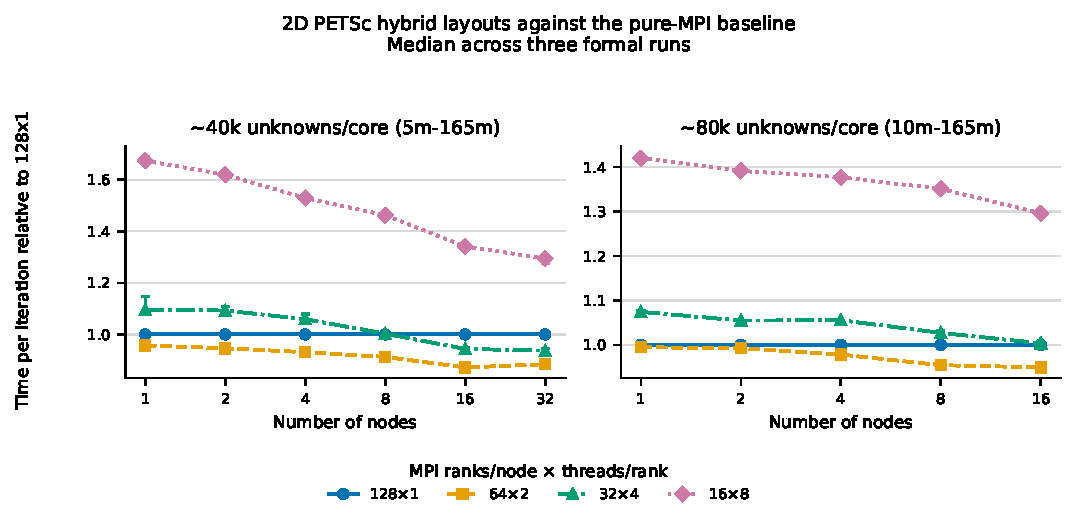
\includegraphics[width=\textwidth]{ksp2d_layout_vs_mpi}
  \caption{2D time per KSP iteration relative to the $128\times1$ baseline at the same
  size--node pair. Values below 1 mean the hybrid layout is faster. Whiskers propagate the
  observed range of three formal runs.}
  \label{fig:2d-ratio}
\end{figure}

Four of the six ratio series are monotone, meaning that the hybrid layout gains on flat MPI
at every step up in node count. Along the $\sim$40k chain, the $64\times2$ ratio falls from
$0.957$ at one node to $0.872$ at 16 before a small reversal to $0.885$ at 32, and
$32\times4$ falls from $1.096$ to $0.937$. Along the $\sim$80k chain all three hybrid
ratios decrease at every step. Thus $64\times2$ is faster per iteration at all 11 pairs,
whereas $32\times4$ crosses the baseline: it costs 9.6\% more at one node, reaches parity
at eight ($1.003$), and costs 6.3\% less at 32. A small-node ranking therefore does not
transfer unchanged.

Raw throughput also includes convergence differences. $64\times2$ leads at eight of 11
pairs. Two of the three flat-MPI leads coincide with one fewer GAMG iteration, and the
third is a 0.4\% tie with overlapping ranges. At 165m on 32 nodes it reaches 794.8 million
equations/s, 13.1\% above flat MPI. Its maxima are a 14.7\% throughput gain and a 12.8\%
time saving at 82m on 16 nodes.

$16\times8$ has the lowest throughput at all 11 pairs, although its deficit narrows from
46.2\% to 22.7\%.

\Cref{fig:2d-spi} shows the corresponding absolute time per iteration.

\begin{figure}[htbp]
  \centering
  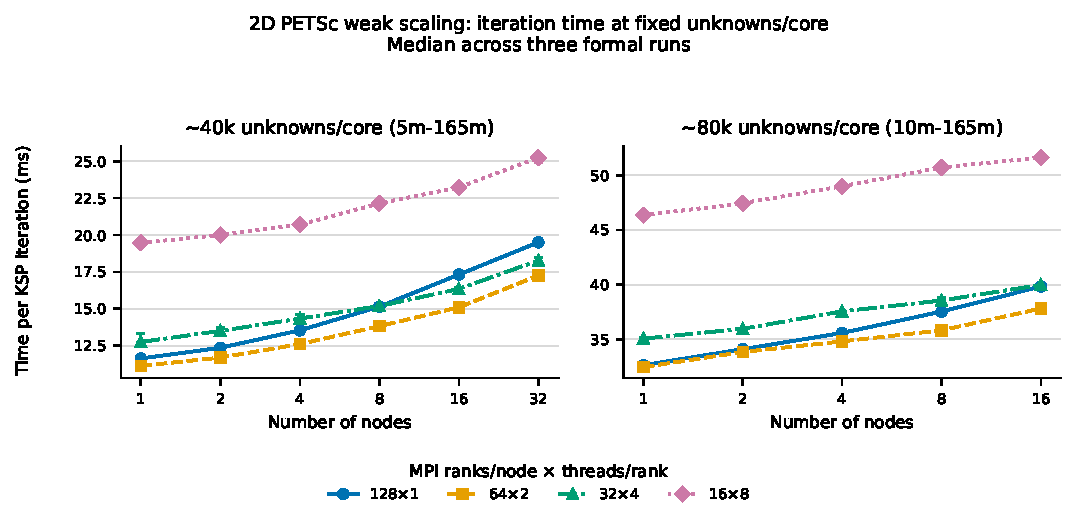
\includegraphics[width=\textwidth]{ksp2d_seconds_per_iteration}
  \caption{Median 2D time per KSP iteration along the two unknowns/core chains. A
  horizontal line would be ideal weak scaling.}
  \label{fig:2d-spi}
\end{figure}

\subsection{3D}
\label{sec:weak-3d}
The 3D campaign uses the same design and takes six or seven KSP iterations. As in 2D,
throughput is near-linear, and the layouts are easier to tell apart once time is normalised
per iteration (\Cref{fig:3d-throughput,fig:3d-ratio}).

\begin{figure}[htbp]
  \centering
  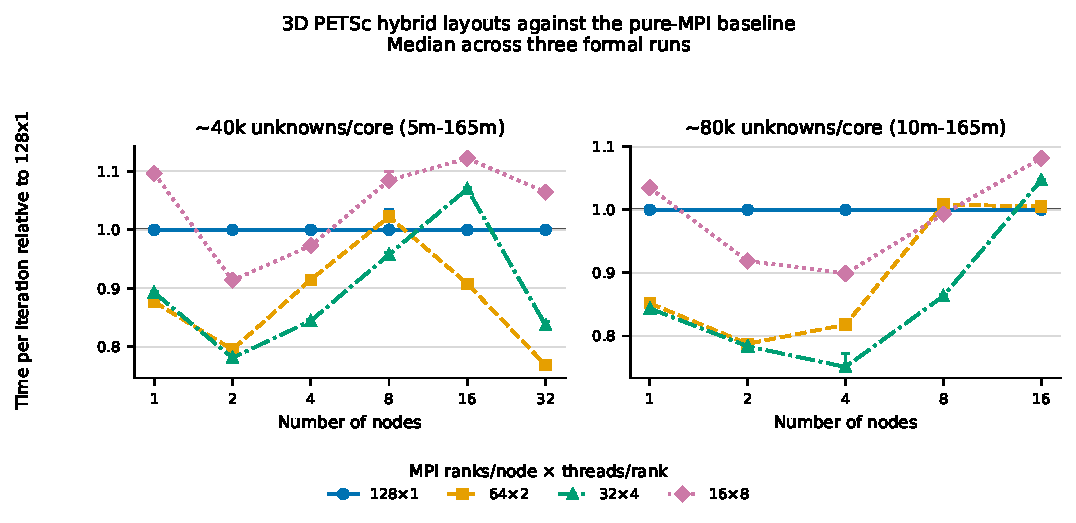
\includegraphics[width=\textwidth]{ksp3d_layout_vs_mpi}
  \caption{3D time per KSP iteration relative to the $128\times1$ baseline at the same
  size--node pair. Unlike the 2D case in \Cref{fig:2d-ratio}, no series is monotone.}
  \label{fig:3d-ratio}
\end{figure}

The 3D advantage is larger but less ordered. At 41m on four nodes, $32\times4$ gives the
largest time saving (24.9\%) and throughput gain (33.2\%); the corresponding 2D maxima are
12.8\% and 14.7\%. These percentages differ because one compares time and the other rate.
Twenty-two of 33 hybrid measurements beat flat MPI per iteration, against 13 of 33 in 2D.
% Both conventions appear in the literature and both appear in this chapter, so they are
%   stated explicitly here once. VERIFIED 2026-08-02 from
%   analysis/data/nproc_2d_libsci/tables/cross_dimension_summary.csv: the maximum time
%   saving and the maximum throughput gain fall at the SAME point in both dimensions
%   (2D 64x2 at 82m/16n, 3D 32x4 at 41m/4n), which is why 12.8/14.7 and 24.9/33.2 pair up.
% VERIFIED 2026-07-31 from repeated_fullnode_formal_summary.csv (both dimensions):
%   ratio<1 counts are 3D 22/33 (64x2 8/11, 32x4 9/11, 16x8 5/11) and 2D 13/33
%   (64x2 11/11, 32x4 2/11, 16x8 0/11).

All six 3D ratio series are non-monotone. On the $\sim$80k chain hybrid layouts are
strongest at two and four nodes, with $32\times4$ reaching $0.784$ and $0.751$, then reach
or exceed parity at 16, where flat MPI is fastest per iteration. On the $\sim$40k chain,
$64\times2$ recovers from $1.022$ at eight nodes to $0.768$ at 32. The advantage is
therefore larger than in 2D but less transferable between node counts.

Raw throughput selects $32\times4$ at six pairs, $64\times2$ at four, and flat MPI at one.
At 165m on 32 nodes, $64\times2$ reaches 510.4 million equations/s, 30.1\% above flat MPI.
$16\times8$ wins no pair but beats flat MPI at five.

\Cref{fig:3d-spi} gives absolute time per iteration.

\begin{figure}[htbp]
  \centering
  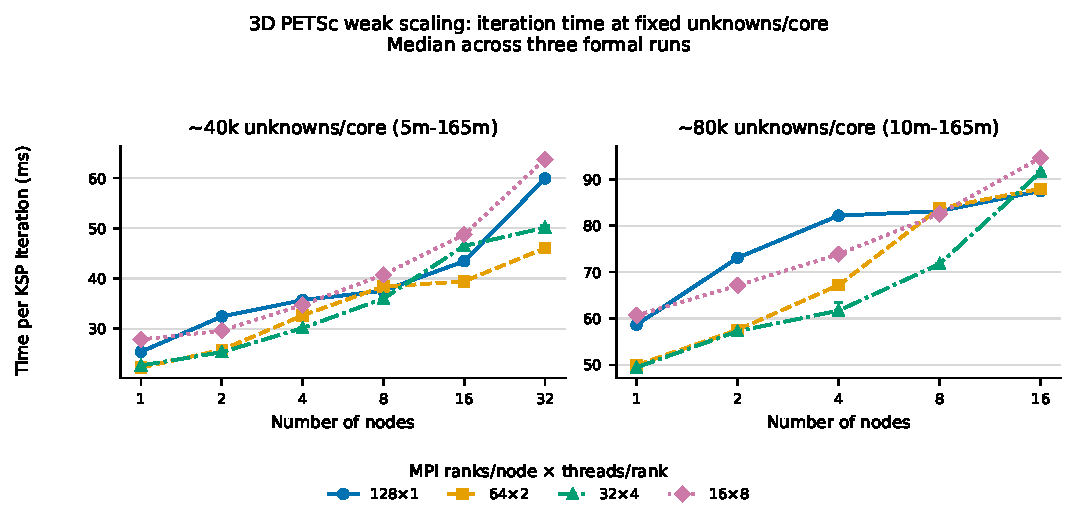
\includegraphics[width=\textwidth]{ksp3d_seconds_per_iteration}
  \caption{Median 3D time per KSP iteration along the two unknowns/core chains.}
  \label{fig:3d-spi}
\end{figure}

\subsection{Layout Ranking and Efficiency}
\label{sec:weak-ranking}
\Cref{tab:weak-best} gives the fastest layout and its margin over flat MPI at every pair.

\begin{table}[htbp]
  \centering
  \caption{Fastest layout by median throughput over three repeats, its margin over flat
  MPI, and time per iteration. The 2D 41m/8-node row is a tie because ranges overlap.}
  \label{tab:weak-best}
  \small
  \begin{tabular}{lrrlrrr}
    \toprule
    Scale & Nodes & Cores & Best layout & M eq/s & vs.\ MPI & ms/iteration \\
    \midrule
    \multicolumn{7}{l}{\emph{2D, five-point stencil}} \\
    5m   &  1 &  128 & $128\times1$ &  47.9 &  0.0\% & 11.63 \\
    10m  &  1 &  128 & $128\times1$ &  34.0 &  0.0\% & 32.63 \\
    10m  &  2 &  256 & $64\times2$  &  94.9 &  5.7\% & 11.69 \\
    20m  &  2 &  256 & $64\times2$  &  59.8 &  0.8\% & 33.84 \\
    20m  &  4 &  512 & $64\times2$  & 160.7 &  7.4\% & 12.60 \\
    41m  &  4 &  512 & $64\times2$  & 107.0 &  2.2\% & 34.81 \\
    41m  &  8 & 1024 & $128\times1$ & 270.5 &  0.0\% & 15.14 \\
    82m  &  8 & 1024 & $64\times2$  & 208.9 &  4.8\% & 35.82 \\
    82m  & 16 & 2048 & $64\times2$  & 495.6 & 14.7\% & 15.10 \\
    165m & 16 & 2048 & $64\times2$  & 362.6 &  5.3\% & 37.82 \\
    165m & 32 & 4096 & $64\times2$  & 794.8 & 13.1\% & 17.25 \\
    \addlinespace
    \multicolumn{7}{l}{\emph{3D, seven-point stencil}} \\
    5m   &  1 &  128 & $64\times2$  &  37.4 & 14.1\% & 22.26 \\
    10m  &  1 &  128 & $32\times4$  &  28.7 &  1.6\% & 49.45 \\
    10m  &  2 &  256 & $64\times2$  &  64.3 & 25.8\% & 25.78 \\
    20m  &  2 &  256 & $32\times4$  &  50.8 & 27.6\% & 57.26 \\
    20m  &  4 &  512 & $32\times4$  &  96.5 &  1.5\% & 30.13 \\
    41m  &  4 &  512 & $32\times4$  &  95.1 & 33.2\% & 61.68 \\
    41m  &  8 & 1024 & $32\times4$  & 163.0 &  4.4\% & 35.99 \\
    82m  &  8 & 1024 & $32\times4$  & 163.9 & 15.8\% & 71.75 \\
    82m  & 16 & 2048 & $64\times2$  & 298.2 & 10.2\% & 39.44 \\
    165m & 16 & 2048 & $128\times1$ & 268.8 &  0.0\% & 87.47 \\
    165m & 32 & 4096 & $64\times2$  & 510.4 & 30.1\% & 46.06 \\
    \bottomrule
  \end{tabular}
\end{table}
% VERIFIED 2026-08-03 by analysis/scripts/cross_dimension/summarize_best_layouts.py ->
%   analysis/data/nproc_2d_libsci/tables/weak_scaling_best_layouts.csv. It reads both
%   repeated_fullnode_formal_summary.csv files, raises unless each carries 11 size--node
%   pairs with all four layouts, and picks the layout with the highest median throughput.
%   It reproduces every headline figure quoted in this chapter from the raw campaign:
%   2D 64x2 wins 8 of 11 and peaks at 14.7% and 794.8 Meq/s; 3D 32x4 wins 6 of 11,
%   64x2 4 and flat MPI 1, peaking at 33.2% (41m/4n) and 510.4 Meq/s / 30.1% (165m/32n).

The 2D winner changes twice across the 11 rows. The 3D winner changes five times. This
matches the ordered 2D and scale-dependent 3D ratio trends.

Taking each layout's own single-node time as its baseline gives the weak-scaling
efficiencies in \Cref{tab:weak-eff}.

\begin{table}[htbp]
  \centering
  \caption{Weak-scaling efficiency (\%) at the largest node count of each chain, relative
  to the same layout's one-node time. Each layout is measured against itself, so this
  quantifies degradation, not absolute speed.}
  \label{tab:weak-eff}
  \begin{tabular}{llrrrr}
    \toprule
    & & \multicolumn{4}{c}{Layout} \\
    \cmidrule(lr){3-6}
    Case & Chain and node count & $128\times1$ & $64\times2$ & $32\times4$ & $16\times8$ \\
    \midrule
    2D & $\sim$40k, 32 nodes & 59.6 & 64.5 & 69.8 & 77.1 \\
    2D & $\sim$80k, 16 nodes & 81.9 & 85.8 & 87.7 & 89.8 \\
    3D & $\sim$40k, 32 nodes & 42.4 & 48.3 & 45.2 & 43.7 \\
    3D & $\sim$80k, 16 nodes & 67.0 & 56.8 & 54.0 & 64.1 \\
    \bottomrule
  \end{tabular}
\end{table}

In 2D, efficiency rises with threads per rank in both chains. This tracks the falling ratio
curves but does not rank absolute speed: $16\times8$ has the best efficiency and the worst
time at every point. A metric based on each layout's own baseline can reward a poor
baseline.

The 3D efficiencies have no thread-count ordering: $64\times2$ leads the $\sim$40k chain,
whereas flat MPI leads the $\sim$80k chain. The 2D pattern does not transfer.

\section{Strong Scaling at Fixed Problem Size}
\label{sec:strong}
The fixed-size campaign asks where additional nodes stop reducing runtime. Both dimensions
use the same six node counts and four layouts.

\subsection{2D}
\label{sec:strong-2d}
The five local 2D doublings give speedups of 2.00--3.08. Superlinear steps repeat within
the three-run sample, but their cause is not identified.

All 2D fixed-size curves still improve at 32 nodes (\Cref{fig:2d-strong20m}). The
fastest-to-slowest spread grows from $1.47\times$ at one node to $1.81\times$ at 16, then
narrows to $1.48\times$. $64\times2$ is fastest at nodes $\{2,4,8,32\}$ and flat MPI at
$\{1,16\}$. Cumulative efficiency peaks at 191\% for $64\times2$ at eight nodes; cache
capacity and GAMG hierarchy changes remain untested explanations for this superlinearity.

\begin{figure}[htbp]
  \centering
  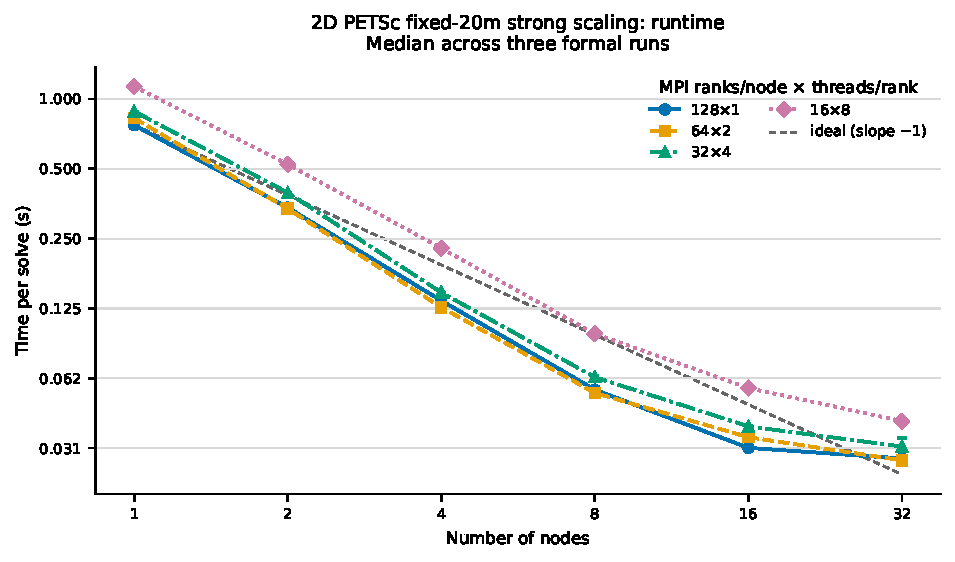
\includegraphics[width=0.85\textwidth]{ksp2d_strong20m_runtime}
  \caption{2D time per solve at a fixed 20.25M unknowns, one to 32 nodes. Both axes are
  logarithmic, so ideal strong scaling is a straight line of slope $-1$. Whiskers show the
  observed range of three formal runs.}
  \label{fig:2d-strong20m}
\end{figure}

\subsection{3D}
\label{sec:strong-3d}
The five local 3D doublings give speedups of 1.46--2.39, without a superlinear step. At
165m, $64\times2$ gives $1.91\times$ from 16 to 32 nodes, against $1.46\times$ for MPI.

Three 3D layouts reach a minimum time and then get slower again within the measured range
(\Cref{fig:3d-strong20m}). Flat MPI
reaches its minimum at eight nodes, $64\times2$ and $32\times4$ at 16. Only $16\times8$
still improves at 32 nodes, where its 0.0681\,s solve is $3.81\times$ faster than flat MPI
on the same 4096 cores and 10\% faster than $32\times4$. The disjoint ranges support a
layout difference at that endpoint, but the campaign does not locate the later
$16\times8$ saturation point.

\begin{figure}[htbp]
  \centering
  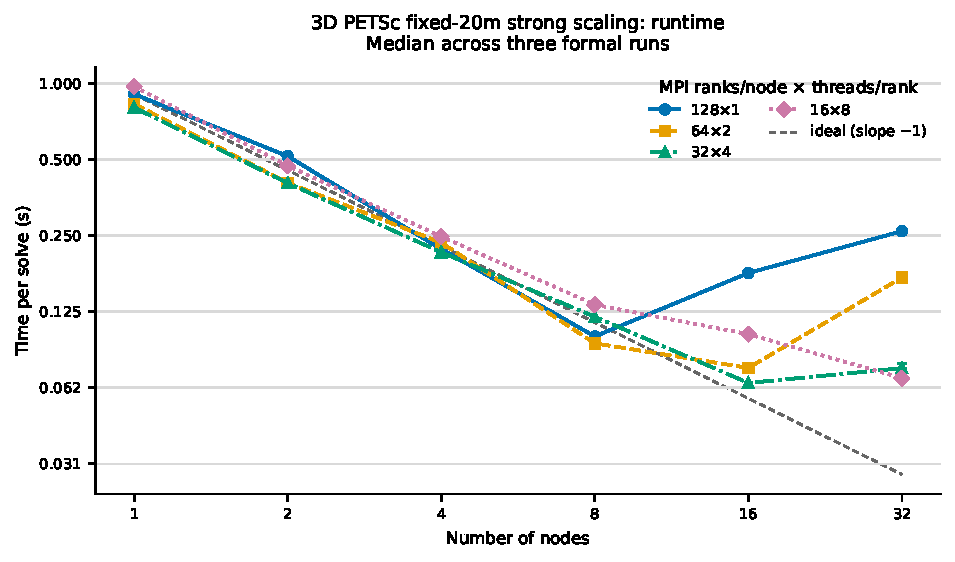
\includegraphics[width=0.85\textwidth]{ksp3d_strong20m_runtime}
  \caption{3D time per solve at a fixed 20.35M unknowns. Flat MPI bottoms at eight nodes,
  $64\times2$ and $32\times4$ at 16, and only $16\times8$ still improves at 32.}
  \label{fig:3d-strong20m}
\end{figure}

\Cref{fig:3d-strong20m-eff} measures each layout against its own one-node time, so it ranks
scaling behaviour rather than speed. \Cref{sec:strong-endpoints} reports both. The 2D
curves do not turn, so their efficiencies remain in \Cref{tab:strong20m-endpoints}.

\begin{figure}[htbp]
  \centering
  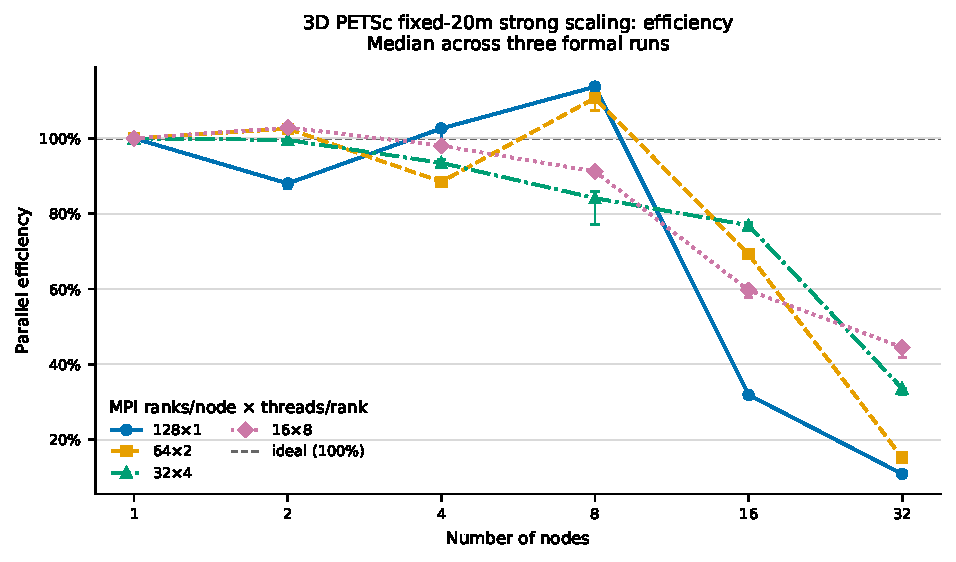
\includegraphics[width=0.85\textwidth]{ksp3d_strong20m_efficiency}
  \caption{3D parallel efficiency at a fixed 20.35M unknowns, each layout against its own
  one-node time. Because the baselines differ, this figure ranks scaling behaviour and not
  speed. Flat MPI falls to 10.9\% at 32 nodes while $16\times8$ retains 44.5\%.}
  \label{fig:3d-strong20m-eff}
\end{figure}

\subsection{Endpoints}
\label{sec:strong-endpoints}
\Cref{tab:strong20m-best} gives the fastest layout and its margin over flat MPI at each
node count. The 2D margin stays below 6.9\%; the 3D margin reaches 281.3\% at 32 nodes.

\begin{table}[htbp]
  \centering
  \caption{Fastest layout for each fixed 20M problem, by three-run median time per solve,
  and its advantage over flat MPI.}
  \label{tab:strong20m-best}
  \begin{tabular}{lrlrrlrr}
    \toprule
    & & \multicolumn{3}{c}{2D, $4500^2$} & \multicolumn{3}{c}{3D, $273^3$} \\
    \cmidrule(lr){3-5}\cmidrule(lr){6-8}
    Nodes & Cores & Best & s/solve & vs.\ MPI & Best & s/solve & vs.\ MPI \\
    \midrule
     1 &  128 & $128\times1$ & 0.7704 &  0.0\% & $32\times4$ & 0.8022 &  13.0\% \\
     2 &  256 & $64\times2$  & 0.3365 &  1.0\% & $32\times4$ & 0.4028 &  27.8\% \\
     4 &  512 & $64\times2$  & 0.1265 &  6.9\% & $32\times4$ & 0.2145 &   2.9\% \\
     8 & 1024 & $64\times2$  & 0.0541 &  3.3\% & $64\times2$ & 0.0936 &   6.5\% \\
    16 & 2048 & $128\times1$ & 0.0313 &  0.0\% & $32\times4$ & 0.0652 & 172.4\% \\
    32 & 4096 & $64\times2$  & 0.0277 &  1.9\% & $16\times8$ & 0.0681 & 281.3\% \\
    \bottomrule
  \end{tabular}
\end{table}

At 32 nodes, 2D speedups cluster at 27.3--29.8 because each layout uses its own one-node
baseline, although endpoint runtimes differ by 45\% (\Cref{tab:strong20m-endpoints}). In
3D the speedup and runtime rankings agree.

\begin{table}[htbp]
  \centering
  \caption{The 32-node endpoint of the fixed-size curves. Speedup and cumulative
  efficiency are measured against the same layout's one-node time, so they reward a poor
  baseline. The doubling efficiency is the 16-to-32-node step alone. Time per solve is the
  only column that compares layouts directly.}
  \label{tab:strong20m-endpoints}
  \begin{tabular}{llrrrr}
    \toprule
    Case & Layout & s/solve & Speedup & Efficiency & 16$\to$32 step \\
    \midrule
    2D & $128\times1$ & 0.0282 & 27.30 & 85.3\% & 55.5\% \\
    2D & $64\times2$  & 0.0277 & 29.83 & 93.2\% & 62.9\% \\
    2D & $32\times4$  & 0.0317 & 27.85 & 87.0\% & 61.1\% \\
    2D & $16\times8$  & 0.0409 & 27.71 & 86.6\% & 69.4\% \\
    \addlinespace
    3D & $128\times1$ & 0.2599 &  3.49 & 10.9\% & 34.2\% \\
    3D & $64\times2$  & 0.1703 &  4.87 & 15.2\% & 22.0\% \\
    3D & $32\times4$  & 0.0747 & 10.75 & 33.6\% & 43.7\% \\
    3D & $16\times8$  & 0.0681 & 14.24 & 44.5\% & 74.6\% \\
    \bottomrule
  \end{tabular}
\end{table}
% VERIFIED 2026-08-01 from analysis/data/nproc_{2d,3d}_libsci/tables/strong_scaling_20m/
%   strong_scaling_20m_{best_layouts,endpoints}.csv, regenerated by
%   analysis/scripts/strong_scaling_20m/analyze_strong_scaling_20m.py.

\section{Interpretation}
\label{sec:mn-interp}
\Cref{tab:cross-dimension} summarises the different trend shapes. The 3D gaps against flat
MPI at 16 and 32 nodes exceed observed run-to-run spreads. The 1--7\% 2D fixed-size margins
do not, so individual 2D rankings remain indicative.

\begin{table}[htbp]
  \centering
  \caption{Cross-dimensional weak- and strong-scaling summary. Throughput gain and time
  saving use rate and time conventions respectively. A layout turns upward when its time
  after its measured minimum increases.}
  \label{tab:cross-dimension}
  \begin{tabular}{lll}
    \toprule
    & 2D & 3D \\
    \midrule
    \multicolumn{3}{l}{\emph{Constant work per core, 11 size--node pairs}} \\
    Layout winning most points        & $64\times2$ (8 of 11) & $32\times4$ (6 of 11) \\
    Hybrid points faster per iteration & 13 of 33 & 22 of 33 \\
    Largest throughput gain           & 14.7\% & 33.2\% \\
    Largest per-iteration saving      & 12.8\% & 24.9\% \\
    Ratio series monotone in nodes    & 4 of 6 & 0 of 6 \\
    Weak efficiency rises with threads & yes & no \\
    \addlinespace
    \multicolumn{3}{l}{\emph{Fixed 20M problem, one to 32 nodes}} \\
    Layouts whose time turns upward   & none of 4 & 3 of 4 \\
    First to turn upward              & --- & $128\times1$, at 8 nodes \\
    Speedup on the last doubling      & $1.11$--$1.39\times$ & $0.44$--$1.49\times$ \\
    Fastest at 32 nodes               & $64\times2$ & $16\times8$ \\
    Its lead over flat MPI            & $1.02\times$ & $3.81\times$ \\
    Fastest-to-slowest spread at 32 nodes & $1.48\times$ & $3.81\times$ \\
    \bottomrule
  \end{tabular}
\end{table}
% VERIFIED 2026-08-05 by analysis/scripts/cross_dimension/summarize_cross_dimension.py ->
%   analysis/data/nproc_2d_libsci/tables/cross_dimension_summary.csv. It joins the two
%   formal summaries, the two strong-scaling summaries and the exposure fits, so no number
%   in this table is transcribed from another chapter by hand. "Turns upward" is
%   saturated_within_range: the layout's minimum time falls before the largest node count.
%   The last-doubling row is strong_last_doubling_speedup_{min,max}, 16 to 32 nodes.

Four of six 2D ratio series are monotone and weak efficiency rises with thread count. No
3D series is monotone, and its preferred layout changes with scale and nodes. Scaling
regime also matters: layout differences are percentage-level at constant work per core but
reach $3.81\times$ for the fixed 3D problem at 32 nodes because layouts saturate at
different measured points.

Because the stencils perform different work per equation, cross-dimensional comparisons
use layout ordering, margins to flat MPI and trend shape, not absolute throughput.

This chapter does not identify the mechanism behind either the improving 2D hybrid ratios
or the poor absolute performance of $16\times8$. \Cref{ch:profiling} tests whether event
exposure and OpenMP waiting track these observations. \Cref{ch:discussion} converts the
combined evidence into recommendations.

A layout recommendation must therefore name its scaling regime. $16\times8$ is last at
constant work per core in both dimensions but first at 4096 cores for the fixed 3D
problem. These measurements answer different questions.

% ===== FILE: chapters/ch6_profiling.tex =====
\chapter{Profiling and Bottleneck Analysis}
\label{ch:profiling}
% §6.4 added 2026-07-31: systematic -log_view event analysis over all 264 formal runs.
% §6.3 rewritten 2026-08-01 against the MAP call-tree analysis (11 usable profiles, two
%   builds). Still outstanding: hardware counters to explain WHY the threads wait.
% Fuller draft: ../dissertation_prep/03_draft_profiling_framework.md.

\section{Why a Repeated-Solve Driver}
\label{sec:whyrepeat}
In a single solve at 20.25M with $16\times8$, \texttt{-log\_view} gave \texttt{PCSetUp}
45\% of time and \texttt{KSPSolve} 10\%. \texttt{ex2\_repeat} runs the solve inside a
\texttt{RepeatedSolves} log stage, zeroes the initial guess before each solve, and reuses
the preconditioner (\texttt{-ksp\_reuse\_preconditioner} and
\texttt{-pc\_gamg\_reuse\_interpolation true}). With 20 solves the stage held 69\% of time
and 93\% of flops; within the stage \texttt{KSPSolve} was 100\% of time; each of the 19
repeats took 11 iterations. The corrected scaling campaign uses this same warm-up and
reuse design, so \Cref{ch:multinode} compares steady-state solves rather than first-touch
and hierarchy-construction costs.

\section{Analysis Methodology}
\label{sec:analysis-method}
The method combines MAP 25.0.4 timelines with \texttt{-log\_view} \%T (share of stage
time) and \%F (share of stage flops). An event whose \%T exceeds its \%F spends the
difference on communication, synchronisation, or memory traffic. \Cref{tab:tf} lists
single-point data for the RepeatedSolves stage at 20.25M with $16\times8$.

\begin{table}[htbp]
  \centering
  \caption{Per-event time and flop shares, RepeatedSolves stage, 20.25M, $16\times8$.}
  \label{tab:tf}
  \begin{tabular}{lrrr}
    \toprule
    Event & \%T & \%F & GF/s \\
    \midrule
    \texttt{MatMult}          & 39 & 55 & 30.5 \\
    \texttt{MatMultTranspose} & 18 &  6 &  6.7 \\
    \texttt{VecTDot+VecNorm}  &  8 &  6 & --   \\
    \texttt{PCApply} (agg.)   & 82 & 82 & 21.6 \\
    \bottomrule
  \end{tabular}
\end{table}

\texttt{MatMultTranspose} (GAMG restriction) has a \%T three times its \%F and a rate
$4.6\times$ below \texttt{MatMult}. \texttt{VecTDot} and \texttt{VecNorm} are the CG global
reductions.

The two instruments answer different questions. Uninstrumented \texttt{-log\_view} runs
cover flat MPI and every hybrid layout, so they provide layout comparisons and named PETSc
event exposure. MAP samples call trees and assigns core-time to PETSc, MPI, OpenMP and
libraries, but cannot launch the 128-rank baseline and perturbs runtime. It is therefore
used to locate where hybrid cores are active or waiting, not to supply scaling times.
Neither output is an additive decomposition of the other: PETSc events are nested and
reported as per-rank maxima, whereas MAP shares partition sampled core-time. Agreement
between their orderings is supporting evidence at the accounting level, not permission to
sum the quantities or infer a hardware cause.

\section{MAP Profiling Results}
\label{sec:map-matrix}
Two MAP campaigns profiled the same 20.25M 2D problem:

\begin{enumerate}
  \item a baseline set on \texttt{arch-omp-opt} at 2, 8 and 16 nodes;
  \item a matching set on the production \texttt{arch-omp-libsci-rome-opt} build at 2 and 8
    nodes.
\end{enumerate}

Neither contains a $128\times1$ cell, because MAP cannot launch 128 MPI ranks per node on
this system, so flat MPI has \texttt{-log\_view} evidence only. Of the twelve profiles,
eleven are used. The 16-node $16\times8$ baseline profile is rejected on its own content:
MAP resolved no library symbols in it, so it carries no cost information.

The solve-window scope keeps only the samples in which cores are inside \texttt{KSPSolve}
and none is inside \texttt{PCSetUp}, which approximates the repeated-solve phase from the
profile alone. It is a time window, not the PETSc \texttt{RepeatedSolves} logging stage, and
the two must not be quoted as the same quantity. \Cref{tab:map-shares} gives the resulting
shares and \Cref{fig:map-shares} plots them.

\begin{table}[htbp]
  \centering
  \caption{Share of total core-time inside the solve window, by the library owning the
  executing frame, for the eleven usable MAP profiles at 20.25M unknowns in 2D. OpenMP is
  the GNU runtime's spin and wait paths, that is threads with no work. MAP instrumentation
  inflates these runs, so the ordering between layouts is the result; the absolute values do
  not transfer to the uninstrumented campaigns.}
  \label{tab:map-shares}
  \begin{tabular}{llrrrrr}
    \toprule
    Build & Nodes & Layout & PETSc & OpenMP & MPI & LibSci \\
    \midrule
    LibSci   &  2 & $64\times2$ & 31.9\% & 36.5\% & 29.9\% & 1.0\% \\
    LibSci   &  2 & $32\times4$ & 51.6\% & 40.1\% &  5.8\% & 1.7\% \\
    LibSci   &  2 & $16\times8$ & 42.2\% & 53.5\% &  1.4\% & 2.1\% \\
    \addlinespace
    LibSci   &  8 & $64\times2$ &  4.5\% & 48.3\% & 46.7\% & 0.2\% \\
    LibSci   &  8 & $32\times4$ &  7.5\% & 69.3\% & 22.6\% & 0.3\% \\
    LibSci   &  8 & $16\times8$ & 15.6\% & 76.5\% &  6.2\% & 1.0\% \\
    \addlinespace
    Baseline &  2 & $32\times4$ & 51.7\% & 40.8\% &  6.7\% & 0.0\% \\
    Baseline &  2 & $16\times8$ & 40.2\% & 57.8\% &  1.4\% & 0.0\% \\
    Baseline &  8 & $32\times4$ &  8.8\% & 68.6\% & 22.2\% & 0.0\% \\
    Baseline &  8 & $16\times8$ & 16.0\% & 77.5\% &  6.0\% & 0.0\% \\
    Baseline & 16 & $32\times4$ &  1.2\% & 69.8\% & 29.0\% & 0.0\% \\
    \bottomrule
  \end{tabular}
\end{table}

\begin{figure}[htbp]
  \centering
  \includegraphics[width=\textwidth]{map_solve_window_shares}
  \caption{Where the cores are during the solve, from the MAP call trees. Within each panel
  the OpenMP waiting share grows and the MPI share shrinks as threads replace ranks, and
  both effects strengthen with node count. Paired bars are the two PETSc builds at the same
  configuration.}
  \label{fig:map-shares}
\end{figure}

The two costs trade against each other. The MPI share falls as threads replace ranks: at
eight nodes it goes 46.7\%, 22.6\% and 6.2\% across $64\times2$, $32\times4$ and
$16\times8$. That is the ordering \Cref{sec:bottleneck} obtains from \texttt{-log\_view} on
the whole formal matrix, and MAP is consistent with it at the event-accounting level. Time
in the OpenMP runtime runs the other way, 48.3\%, 69.3\% and 76.5\%, and it is not useful
work: the frames are \texttt{cpu\_relax}, \texttt{do\_spin} and \texttt{\_\_futex\_wait},
that is threads waiting for something to do. The two builds agree wherever they overlap.
Across the four common cells the MPI shares differ by at most 0.9 percentage points and the
OpenMP shares by at most 4.3, with no systematic sign.

MAP's limits bound all of this. There is one profile per cell, so there is no observed
range. The overhead is large and uneven, separately measured at $+35\%$ on the timed stage
and roughly threefold on \texttt{VecScatterEnd}, and the OpenMP instrumentation perturbs the
barrier behaviour being measured, so the absolute percentages overstate what an
uninstrumented run would show.

Within those limits the table answers a question \Cref{ch:multinode} could not, at the level
of accounting rather than of mechanism. The cost that grows with threads per rank, and that
hybridisation has to repay before it pays off, is spent idle in the OpenMP runtime: what
grows is time in \texttt{cpu\_relax}, \texttt{do\_spin} and \texttt{\_\_futex\_wait}, not
time in the compute kernels. NUMA placement is excluded on topology alone. A rank of eight
threads crosses a shared-L3 boundary but still fits inside one 16-core NUMA region, so no
layout in this study puts a rank across two NUMA regions and the four cannot differ in that
respect (\Cref{tab:layouts}).

Nor is the growth a placement effect, because it is present at a fixed layout, where a
rank's threads occupy the same cores against the same shared-L3 boundary at every node
count. Holding $16\times8$ fixed and going from two nodes to eight raises the waiting share
from 53.5\% to 76.5\% on the LibSci build and from 57.8\% to 77.5\% on the baseline, as the
work per threaded region shrinks.

The other two features of the shape, monotonicity in the thread count and a maximum exactly
where $16\times8$ performs worst, are consistent with that same explanation, that each
threaded region holds less work. They are equally consistent with a cache explanation, in
which a rank spanning two CCXs produces an imbalance that the same barriers collect. The
profiles cannot separate the two, so why the threads wait is left to the hardware counters
of \Cref{sec:futurework}, as \Cref{sec:sync-limits} sets out. \Cref{sec:bottleneck} shows
the other half of the trade, on the full matrix and without a profiler.

The last observation is negative and worth stating. Threaded LibSci is linked into the
production build, and PETSc's sparse solve path barely calls it: BLAS accounts for at most
2.1\% of solve-window core-time in any LibSci profile, and the baseline profiles sample no
BLAS frame at all. The threaded BLAS library therefore cannot account for the layout
ordering measured in \Cref{ch:multinode}, which confirms from profile data what
\Cref{sec:threats} could previously only state as a limit of the evidence.

% BACK-REFERENCE SWEEP 2026-08-09, after the "are consistent with this reading" fix, looking
%   for the same fault everywhere else: a demonstrative or a defined term whose antecedent is
%   not on the page. Six found and fixed, no number touched.
%   (1) sec:sync-tradeoff opened a paragraph "This accounts descriptively for two patterns
%       left by Ch4" -- and it opened it immediately after a figure float, so "This" competed
%       with the figure the reader had just looked at. Now "The relationship between
%       ExposureRemoved and TimeRatio accounts descriptively for ...".
%   (2) sec:sync-limits opened "Pooling all 33 hybrid measurements of a dimension breaks THE
%       RELATIONSHIP" as its first sentence, so the antecedent was in the previous
%       subsection. Now names the two quantities. "breaks it differently in each" also gained
%       its noun, "in each dimension".
%   (3) sec:solver "Time per outer KSP iteration CONTROLS that convergence variation" was the
%       last surviving "controls", which reads as statistical control. sec:threats had the
%       same verb fixed earlier today; this one was missed. Now "Reporting time per outer KSP
%       iteration takes that convergence variation out". grep confirms zero left.
%   (4) The ABSTRACT used "solve-window core-time". Solve window is defined in sec:map-matrix,
%       two hundred pages later in reading order, and an abstract has to stand alone. Now
%       "core time during the solve", matching the wording sec:conclusions already uses.
%   (5) sec:strong20m used "the admission window of sec:configspace" at its first appearance
%       in the document, with no gloss. Now "well outside the 25--100 thousand admitted by
%       sec:configspace", which states the quantity where the reader first meets it. Later
%       uses in sec:rq2 and sec:threats keep the term, which is now glossed twice before them.
%   CHECKED AND LEFT ALONE: "the trade" (defined at sec:motivation and used consistently),
%   "the former/the latter" (no occurrences), gapped verbs before a full stop, and pronouns
%   with two competing antecedents -- the six candidates the scan raised all resolve on the
%   same line. ExposureRemoved, TimeRatio and BreakEven are each first used inside the
%   display equation that defines them, which is the right order.
% MERGED 2026-08-09 with Leyan's own draft of this section, on request. Their structure is
%   adopted almost entirely, and it is better than what it replaces: the two campaigns as a
%   numbered list, the .map-file mechanics dropped, and the argument reordered so the
%   FIXED-LAYOUT observation carries the weight rather than the cross-layout ordering.
%   The .map paragraph deleted on request described how the XML is parsed and how active
%   cores are summed over call-tree leaves. It was method for reproducing the table, not
%   evidence for any claim, and the script is named in app:regen.
%   FIVE THINGS FROM THE DRAFT WERE NOT TAKEN, each for a stated reason:
%   (1) "reproduced here by a different instrument on a different quantity" was NOT restored
%       for the MPI ordering, and the weaker "MAP is consistent with it at the
%       event-accounting level" stands. The 2026-08-07 note at sec:sync-limits records why:
%       the MPI core-time share has a structural ceiling of 1/(threads per rank) if MPI is
%       only ever issued from the master thread -- 50/25/12.5% against measured
%       46.7/22.6/6.2 -- so that ordering may be partly arithmetic and "different quantity"
%       would overstate the independence. The draft's own emphasis on the fixed-layout
%       observation is the right response and IS taken: that one is unaffected, because the
%       ceiling is constant when the layout is held fixed.
%   (2) \includegraphics{figures/map_solve_window_shares} -> bare filename. \graphicspath is
%       {figures/} and a path into the tree is exactly what broke the build once before.
%   (3) The figure had no \Cref anywhere in the draft. House rule: a figure nobody points at
%       gets cut. Restored "\Cref{tab:map-shares} gives the resulting shares and
%       \Cref{fig:map-shares} plots them", and the figure now precedes the discussion it
%       supports rather than sitting after it.
%   (4) Table caption: kept "MAP instrumentation inflates these runs, so the ordering
%       between layouts is the result; the absolute values do not transfer". That is the
%       scope limit on every number in the table and the draft had dropped it. The figure
%       caption likewise keeps the sentence explaining the paired bars.
%   (5) \Cref{sec:sync-limits} in the closing LibSci sentence -> \Cref{sec:threats}, which is
%       where the LibSci limitation was actually stated. sec:sync-limits is about pooling.
%   RESTORED, because the table cannot be read without it: "Of the twelve profiles, eleven
%   are used", with the one-line reason. The draft dropped it, but the table has an 11th row
%   and an asymmetric baseline block, and a reader counting 3+3 LibSci and 5 baseline cells
%   has no way to know why 16-node 16x8 is absent. The Baseline 16-node 32x4 row was also
%   missing from the draft's table and is restored; without it the table has ten rows against
%   a caption saying eleven.
%   \texttt{KSPSolver} -> \texttt{KSPSolve}, and "ignore PCSetUp" -> "none is inside
%   PCSetUp", which is what the filter actually does.
%   The draft's inline "%run another one to solve this!!!" is NOT actionable and was not
%   carried over: MAP cannot launch 128 ranks per node on this system, which is the reason
%   the cell is missing in the first place, not a scheduling accident.


% VERIFIED 2026-08-01 by analysis/scripts/map_profiles/analyze_map_profiles.py, which
%   parses the gzipped MAP XML directly (no Forge licence, no `map --export`), validates
%   each profile against its recorded srun line, and RAISES if the solve-window OpenMP
%   share is not increasing in threads/rank or the MPI share not decreasing. Output:
%   analysis/data/nproc_2d_libsci/csv/derived/map_profiles/map_call_tree_shares.csv and
%   .../reports/map_profile_analysis.md. Rows sum to under 100%: libc, the loader and the
%   sampler make up the small "other" remainder, which is omitted from the table.

\section{Bottleneck Identification}
\label{sec:bottleneck}
\Cref{sec:map-matrix} leaves the hardware question open, but the \texttt{-log\_view} event
tables of the uninstrumented formal runs support a narrower question that
\Cref{ch:multinode} raised and could not answer: whether the layout effect tracks the share
of the solve exposed to inter-process synchronisation. All 264 formal runs are parsed here,
so the evidence covers the same matrix as the scaling results and carries no profiler
overhead.

\subsection{What is Measured}
\label{sec:sync-measured}
For each run, the time of the halo-exchange events (\texttt{VecScatterBegin},
\texttt{VecScatterEnd}) and of CG's global-reduction events (\texttt{VecTDot},
\texttt{VecNorm}) is taken from the \texttt{RepeatedSolves} stage and divided by that
stage's \texttt{KSPSolve} time. 
Three limits apply and none is removable from
\texttt{-log\_view} alone.
First, the synchronising events are logged \emph{inside}
\texttt{MatMult} and its relatives, so this is an exposure share and not a term in an
additive time budget. Summing every non-container event against \texttt{KSPSolve} gives
116--372\%, because \texttt{MatMult} and its relatives are themselves containers for the
halo exchange: the same wait is counted once in \texttt{MatMult}, once in the
\texttt{VecScatter} pair, and once in \texttt{SFPack}/\texttt{SFUnpack}.

Second, each event time is a maximum over ranks, and different events may attain their
maximum on different ranks, so the numerator sums maxima that need not be attained on the
rank supplying the denominator. Third, \texttt{VecTDot} and \texttt{VecNorm} also perform
local flops, so their time is not purely communication.

The quantity is nevertheless measured identically in
every run, so it remains comparable across layouts and node counts.
% VERIFIED 2026-07-31 by analysis/scripts/nproc_2d_libsci/analyze_event_breakdown.py.
%   It also asserts that SFPack/SFUnpack have call counts identical to
%   VecScatterBegin/End (they are nested inside them) and excludes them, because
%   counting both double-counts the halo exchange by roughly a third.

\subsection{Halo Exchange Dominates the Exposure, and Hybridisation Reduces It}
\label{sec:sync-halo}
\Cref{fig:2d-sync} and \Cref{fig:3d-sync} give the result. In both dimensions the share
rises monotonically with node count for every layout and along each weak-scaling chain
separately, and at 21 of the 22 size--node points it is strictly ordered by MPI rank count:
fewer ranks, less exposure. The chains are panelled apart because they do not coincide: the
smaller per-core problem is the more exposed one, by up to 15.5 percentage points in 2D and
8.5 in 3D at the same node count, a difference comparable to the layout separation the
figure exists to show. The plotted share is
the sum of the two event classes, which sit on disjoint call paths: the halo exchange is
reached from \texttt{MatMult} and its relatives, the reductions directly from CG. 
\begin{figure}[htbp]
  \centering
  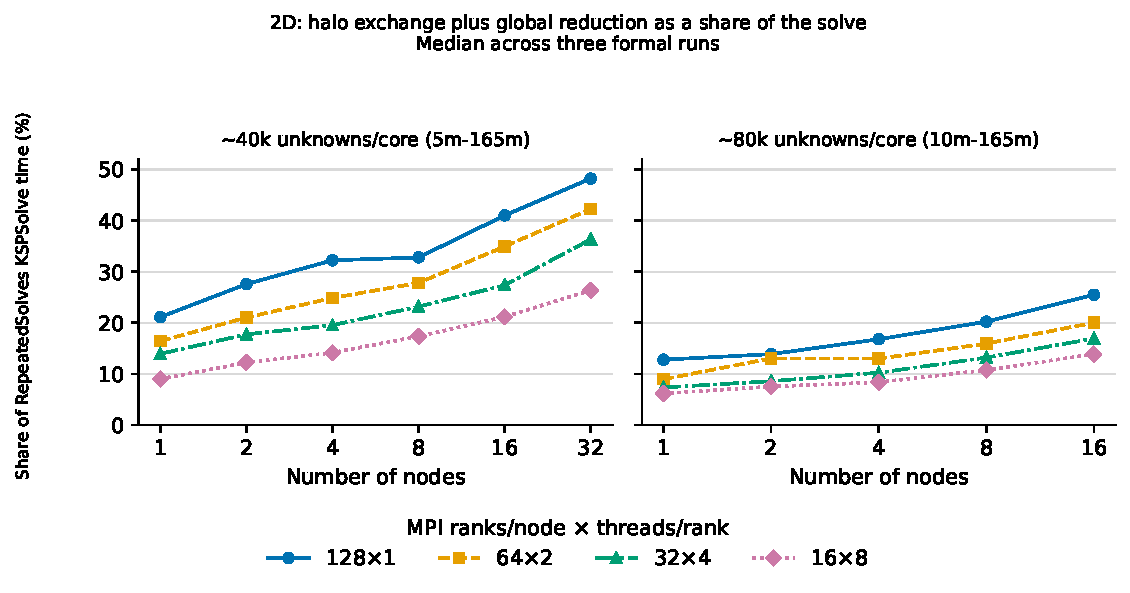
\includegraphics[width=0.85\textwidth]{ksp2d_sync_share}
  \caption{2D share of \texttt{RepeatedSolves} \texttt{KSPSolve} time spent inside halo
  exchange and global reduction events, panelled by unknowns/core chain as in
  \Cref{ch:multinode}. Only the 40k chain reaches 32 nodes. Each point is the median of
  three repetitions. The ordering matches the time-per-iteration ordering in
  \Cref{fig:2d-ratio} at every node count.}
  \label{fig:2d-sync}
\end{figure}

\begin{figure}[htbp]
  \centering
  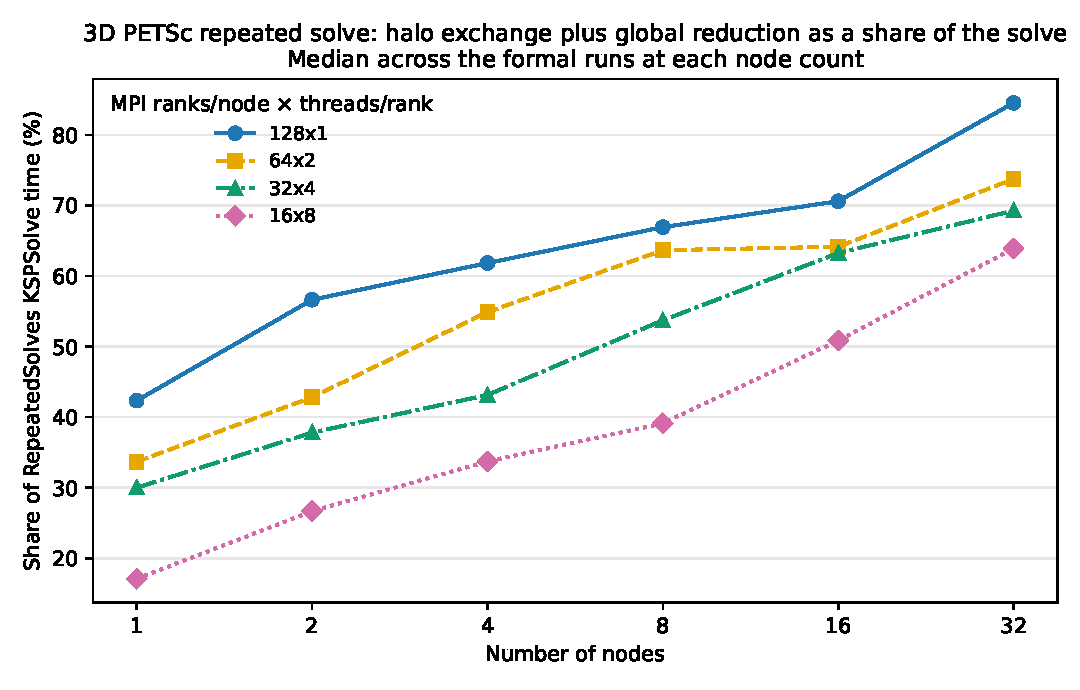
\includegraphics[width=0.85\textwidth]{ksp3d_sync_share}
  \caption{3D share of \texttt{RepeatedSolves} \texttt{KSPSolve} time spent inside halo
  exchange and global reduction events, panelled and styled as in \Cref{fig:2d-sync}.
  Note the vertical scale: flat MPI reaches 84.6\% at the largest point.}
  \label{fig:3d-sync}
\end{figure}



The figures plot only that sum. \Cref{tab:sync-split} separates it at four representative
points along the $\sim$40k unknowns/core chain in each dimension, the chain that reaches 32
nodes. Halo exchange is the larger term in all sixteen cells, by a factor of 1.7 to 2.9 in
2D and 2.9 to 5.7 in 3D. At 165m on 32 nodes flat MPI pays 34.3 percentage points to halo
exchange in 2D and 70.9 in 3D, against 13.9 and 13.6 to the reductions. The totals these
make up are the 48.2\% and 84.6\% at the right-hand end of \Cref{fig:2d-sync} and
\Cref{fig:3d-sync}. The 3D shares are far higher than the 2D shares at every point in the
table, which is what the decomposition of \Cref{sec:benchmarks} predicts: in 3D the
$\pm mn$ coupling puts both $k$ neighbours of every row off-rank once $L$ drops below $mn$,
while in 2D the matching $\pm m$ coupling never reaches more than $2m$ rows.

\begin{table}[htbp]
  \centering
  \caption{The exposure share of \Cref{fig:2d-sync} and \Cref{fig:3d-sync} split into its
  two event classes, at four representative points along the $\sim$40k unknowns/core chain
  of \Cref{tab:bands}, for the $128\times1$ and $16\times8$ layouts. Halo is
  \texttt{VecScatterBegin} and \texttt{VecScatterEnd}; reduction is \texttt{VecTDot} and
  \texttt{VecNorm}. Their sum is the quantity plotted, so it is left to the figures. Each row
  is the repetition whose total is the median of its three, so both components come from the
  same run. The two are rounded independently and at one decimal need not sum to the plotted
  total (3D, 32 nodes, $128\times1$: 70.9 and 13.6 against a plotted 84.6). Percentage points
  of \texttt{RepeatedSolves} \texttt{KSPSolve} time.}
  \label{tab:sync-split}
  \begin{tabular}{llrrrr}
    \toprule
    & & \multicolumn{2}{c}{$128\times1$} & \multicolumn{2}{c}{$16\times8$} \\
    \cmidrule(lr){3-4}\cmidrule(lr){5-6}
    Case & Nodes (size) & Halo & Reduction & Halo & Reduction \\
    \midrule
    2D &  1 (5m)    & 15.7 &  5.4 &  6.1 &  2.9 \\
    2D &  8 (41m)   & 23.4 &  9.4 & 11.2 &  6.1 \\
    2D & 16 (82m)   & 28.6 & 12.4 & 13.6 &  7.6 \\
    2D & 32 (165m)  & 34.3 & 13.9 & 16.4 &  9.9 \\
    \addlinespace
    3D &  1 (5m)    & 35.1 &  9.9 & 15.3 &  4.6 \\
    3D &  8 (41m)   & 53.0 & 18.1 & 38.8 &  6.8 \\
    3D & 16 (82m)   & 59.0 & 15.8 & 46.5 & 10.8 \\
    3D & 32 (165m)  & 70.9 & 13.6 & 52.4 & 11.5 \\
    \bottomrule
  \end{tabular}
\end{table}
% VERIFIED 2026-08-05 from analysis/data/nproc_{2d,3d}_libsci/tables/
%   repeated_fullnode_event_shares.csv, columns neighbour_pct and reduction_pct, whose sum
%   is the sync_pct plotted in fig:2d-sync and fig:3d-sync. "Halo exchange is the larger
%   term" checked over ALL 264 rows (132 per dimension = 4 layouts x 11 size-node points x
%   3 repetitions): neighbour_pct > reduction_pct in every one, ratio range 1.16-3.32 in 2D
%   and 2.33-6.32 in 3D. The chain shown is the ~40k one of tab:bands, the one carrying the
%   165m 32-node point quoted in the text.
%   CAUTION 3 (2026-08-06): the text no longer quotes those 264-run ranges. A reader cannot
%   check a 264-row range against a 16-cell table, and none of the four extreme rows is even
%   shown here (they sit on the ~80k chain, on 64x2, on the 2- and 4-node points, or on a
%   non-median repetition). The text now quotes 1.7-2.9 (2D) and 2.9-5.7 (3D), the same
%   ratio taken over these 16 cells only, and says "larger term in all sixteen cells".
%   One decimal is deliberate: unrounded, the 16-cell range is 1.652-2.929 and 2.921-5.681,
%   while dividing the printed 1-dp values gives 1.66-2.91 and 2.93-5.71. Those agree at one
%   decimal and disagree at two, so two decimals would be uncheckable off the page.
%   CAUTION 4 (2026-08-06): the table shows FOUR of the chain's six points (1, 8, 16, 32),
%   and the caption says "four representative points" rather than implying the whole chain.
%   Nothing in the text or caption now claims anything about the two omitted points. Their
%   values, halo/reduction for 128x1 then 16x8, are
%     2D 2 (10m): 21.2 / 6.4, 8.5 / 3.7     2D 4 (20m): 23.8 / 8.4, 9.4 / 4.8
%     3D 2 (10m): 47.3 / 12.9, 25.4 / 6.0   3D 4 (20m): 50.1 / 15.0, 32.4 / 5.6
%   Before restoring them: they expose component-level non-monotonicities (2D 128x1 halo
%   23.8 -> 23.4 from 4 to 8 nodes; 3D 128x1 reduction peaking at 18.1 at 8 nodes) which
%   sec:sync-halo does not cover, as it claims monotonicity of the SUM only.
%   CAUTION 1: rows are the repetition whose sync_pct is the median of its three, NOT the
%   per-column median. Taking medians column by column does not reproduce the totals,
%   because different repetitions attain the median of each component: at 3D 32 nodes
%   128x1 the component medians are 70.94 and 13.13, summing to 84.07, whereas the median
%   total is 84.56. The 84.6 in the text and in the fig:3d-sync caption is the median
%   total and is correct.
%   CAUTION 2: do NOT add a total column back. At one decimal place the printed components
%   do not always sum to the printed total (3D 32 nodes 128x1: 70.9 + 13.6 = 84.5 against a
%   true 70.944 + 13.615 = 84.559, printed 84.6). Six of the sixteen cells in the earlier
%   draft of this table were affected. The total belongs in the figures and, for the points
%   quoted, in the running text. As of 2026-08-06 the caption states this rounding caveat
%   explicitly and names the 3D 32-node case, because the running text had said "70.9 of
%   84.6" while the table printed 70.9 and 13.6, which a reader adds to 84.5. That sentence
%   was rewritten to attribute the totals to the figures instead of to the components.

\subsection{Reduced Exposure is Necessary but not Sufficient}
\label{sec:sync-breakeven}
The ordering alone cannot explain the results, because $16\times8$ has the lowest exposure
at every point of \Cref{fig:2d-sync} and \Cref{fig:3d-sync} and yet, in 2D, the worst time
per iteration at all 11 of them. What does track performance is the \emph{size} of the
reduction, taken within a single layout, which gives the fits in \Cref{tab:sync-breakeven}.

Let $S_\ell$ be the plotted halo-plus-reduction share of layout $\ell$ and $t_\ell$ its time
per KSP iteration, both at the same size--node point. The first two columns of
\Cref{tab:sync-breakeven} are the range, over the 11 points, of
\[
  \mathrm{ExposureRemoved} = S_{128\times1} - S_\ell, \qquad
  \mathrm{TimeRatio} = \frac{t_\ell}{t_{128\times1}},
\]
so $\mathrm{ExposureRemoved}>0$ means the layout is less exposed than flat MPI, and
$\mathrm{TimeRatio}<1$ means it is faster. For example, $\mathrm{ExposureRemoved}$ is
$(34.3+13.9)-(16.4+9.9)=21.9$ points for 2D $16\times8$ at 165m on 32 nodes in
\Cref{tab:sync-split}.

Break-even, a measure defined here, is computed from $a$ and $b$,
\[
  \mathrm{BreakEven} = \frac{1-b}{a} = \frac{b-1}{|a|}, \qquad a<0,
\]
with none when $a\ge0$. These two come from a least-squares fit over each layout's 11 pairs,
\[
  \mathrm{TimeRatio} = a\,\mathrm{ExposureRemoved} + b .
\]
Here $b$ is the intercept, the time ratio the line gives at $\mathrm{ExposureRemoved}=0$:
what a layout would cost against flat MPI if its exposure share matched flat MPI's, so $b-1$
is the cost of threading alone. The slope $a$ is the change in $\mathrm{TimeRatio}$ per point
of $\mathrm{ExposureRemoved}$, so $|a|$ is how much of that cost one point pays back.
% VERIFIED 2026-08-08, VOCABULARY. Raised by Leyan: "removes the most exposure" was
%   unreadable. It meant ExposureRemoved, but three things were wrong with saying it that
%   way. (1) "removes" implies an action, while ExposureRemoved = S_128x1 - S_l is a
%   DIFFERENCE between two layouts at the same point; the definition above says the layout
%   "is less exposed than" flat MPI, a state. (2) bare "exposure" was carrying two meanings
%   in one section -- S_l ("16x8 has the lowest exposure", 22/22) and the gap ("removes the
%   most exposure"). (3) a share cannot be removed, only lowered. Six sites changed, no
%   number touched: the Ch1 contributions item, this paragraph twice, the |a| paragraph,
%   sec:sync-limits twice, sec:rq3, and sec:threats ("removes exposure to" -> "reduces
%   exposure to", the correct collocation).
%   THE RULE, three forms and no fourth:
%     S_l, the layout's own share          -> "exposure share"
%     S_128x1 - S_l, the gap to flat MPI   -> $\mathrm{ExposureRemoved}$, or in Ch6 where the
%                                             symbols are not in play, "sits below flat MPI's
%                                             exposure share"
%     being exposed to an event            -> "exposure TO halo exchange" (idiomatic, keep)
%   NOT changed, deliberately: tab:sync-breakeven's "Exposure removed" column header and the
%   fig:2d-tradeoff/fig:3d-tradeoff axis wording. Those are labels; prose referring to them
%   uses the symbol. The sec:sync-limits paragraph was the odd one out to begin with -- the
%   two paragraphs before it, in sec:sync-breakeven, already use $\mathrm{ExposureRemoved}$
%   throughout, so this aligns it with its neighbours rather than introducing a new style.
%   CORRECTION carried over: the Ch1 contributions item also said "21 of 22 size--node
%   points" for the exposure-reduction claim. That is the THIRD instance of the same
%   borrowing from sec:sync-halo's rank-count ORDERING claim, after sec:sync-breakeven
%   (fixed 2026-08-06) and sec:rq3 (fixed 2026-08-08). It is 22/22 -- all three hybrid
%   layouts have exposure_removed_pt > 0 at 11/11 points in each dimension, and
%   analyze_event_breakdown.py line 398 raises on <= 0. Grep for "21 of" before adding any
%   new sentence about exposure reduction; only sec:sync-halo may carry that number, and
%   only for the four-layout ordering (2D 11/11 + 3D 10/11, the exception being 3D 82m/16n
%   where 64x2 at 68.6 sits below 32x4 at 69.3). Since $a<0$, the
fitted line drops below one exactly where $\mathrm{ExposureRemoved}$ passes
$\mathrm{BreakEven}$. The column is therefore a threshold: it is how much exposure a layout
has to remove before threading pays for itself, and the lower it is, the sooner that
happens. The fit is descriptive, so single points can fall on the wrong side of it.

The $r$ column is the Pearson correlation, computed from the same 11 pairs,
\[
  r = \frac{\operatorname{cov}(\mathrm{ExposureRemoved},\ \mathrm{TimeRatio})}
           {\sigma_{\mathrm{ExposureRemoved}}\ \sigma_{\mathrm{TimeRatio}}},
\]
their covariance over the product of their standard deviations. It shares the sign of $a$
and says how closely they follow the line, so it measures how firm a break-even is rather
than adding an effect of its own.

\begin{table}[htbp]
  \centering
  \caption{$\mathrm{ExposureRemoved}$ against $\mathrm{TimeRatio}$, both relative to flat MPI
  at the same size--node point, the first in percentage points. The break-even value is the
  exposure reduction the fitted line requires to offset threading overhead. $a$ and $b$ are
  that line's slope and intercept, tabulated as $10^3a$, so $(1-b)/a$ reproduces the last
  column. \emph{None} marks $a\ge0$, where the line never descends to parity and no
  break-even exists. Eleven points per layout. The fits are descriptive only.}
  \label{tab:sync-breakeven}
  \begin{tabular}{lrrrrrr}
    \toprule
    Layout & Exposure removed & Time ratio & $r$ & $10^3a$ & $b$ & Break-even \\
    \midrule
    \multicolumn{7}{@{}l}{\emph{2D}}\\
    $64\times2$ &  0.8--7.4  & 0.872--0.995 & $-0.67$ & $-15.29$ & 1.0178 & 1.2 \\
    $32\times4$ &  5.3--13.7 & 0.937--1.096 & $-0.59$ & $-11.13$ & 1.1305 & 11.7 \\
    $16\times8$ &  6.3--21.9 & 1.294--1.674 & $+0.00$ & $+0.08$  & 1.4313 & none \\
    \addlinespace
    \multicolumn{7}{@{}l}{\emph{3D}}\\
    $64\times2$ &  1.9--15.1 & 0.768--1.022 & $-0.86$ & $-21.60$ & 1.0618 & 2.9 \\
    $32\times4$ &  5.5--23.5 & 0.751--1.070 & $-0.90$ & $-17.47$ & 1.1270 & 7.3 \\
    $16\times8$ & 17.4--31.1 & 0.899--1.122 & $-0.83$ & $-15.82$ & 1.4226 & 26.7 \\
    \bottomrule
  \end{tabular}
\end{table}

% VERIFIED 2026-08-06 for the opening sentence of sec:sync-breakeven, from
%   repeated_fullnode_exposure_tradeoff.csv in both dimensions.
%   "lowest exposure at every point": 16x8 has the minimum sync_pct at 11/11 2D points and
%   11/11 3D points, i.e. 22/22. The sentence previously said "nearly every point", which
%   UNDERSTATED it. The "nearly" looks borrowed from sec:sync-halo's "21 of the 22 points
%   strictly ordered by MPI rank count" -- but that is a different claim, about the full
%   four-layout ordering, and its one exception is 3D 82m/16 nodes, where 64x2 (68.6) sits
%   below 32x4 (69.3). 16x8 is still the lowest there. Both statements are correct as they
%   now stand; do not "reconcile" them by weakening this one again.
%   This claim is NOT derivable from tab:sync-breakeven: the Exposure removed ranges overlap
%   (2D 16x8 6.3-21.9 against 32x4 5.3-13.7), so a range comparison proves nothing pointwise.
%   It is read off fig:2d-sync and fig:3d-sync, where 16x8 is the bottom curve in every
%   panel, and the text now cites those two figures for it.
%   "worst time per iteration at all 11 points in 2D": true, 11/11, and this one IS derivable
%   from tab:sync-breakeven because the time-ratio ranges are disjoint -- 16x8 opens at 1.294,
%   above 32x4's close at 1.096, 64x2's at 0.995, and flat MPI's 1.000 by definition. The
%   text now spells that argument out. CAUTION: it holds in 2D ONLY. In 3D 16x8 is slowest at
%   just 6/11 points and its range (0.899-1.122) overlaps both others, so do not generalise
%   the sentence across dimensions.
% VERIFIED 2026-08-06: the defining paragraph above was added because the section used
%   "exposure removed", "time ratio" and "break-even" without defining any of them; only
%   the table caption glossed break-even. Definitions taken from
%   analysis/scripts/nproc_2d_libsci/analyze_event_breakdown.py lines 239-240 and 256-262:
%     exposure_removed_pt = mpi_sync_pct - sync_pct   (NOT a sum -- it is flat MPI's
%       halo+reduction share minus this layout's, at the same scale/nodes point)
%       THRESHOLD IS ZERO, not one: this is a difference of two percentages, in points,
%       while time_ratio is a ratio and its threshold is one. A draft once wrote
%       "ExposureRemoved > 1"; 2D 64x2's range starts at 0.8, a real point that is above 0
%       and below 1, so the two thresholds are not interchangeable. The script asserts
%       positivity for every row (analyze_event_breakdown.py line 398 raises on <= 0).
%     time_ratio          = seconds_per_iteration / mpi_seconds_per_iteration
%     slope a, intercept b = np.polyfit(x, y, 1) over the layout's 11 points
%     break_even x_be      = (1 - b) / a, NaN when a >= 0
%   PROVENANCE OF THE NAME, 2026-08-06: "break-even" is ordinary technical English for the
%   threshold at which two opposing effects cancel, so the term needs no citation, but THIS
%   quantity -- (1-b)/a over the exposure/time-ratio fit -- is not a standard metric from
%   the literature and carries no reference anywhere in the draft. The text therefore says
%   "a measure defined here", so that a reader cannot mistake it for a borrowed one. Keep
%   that clause if the sentence is reworded.
%   ROLE, added 2026-08-06: for a<0, "TimeRatio < 1" and "ExposureRemoved > BreakEven" are
%   the same condition ON THE FITTED LINE, which is why the column reads as a threshold.
%   It is NOT exact on the measured points, and the text says so ("single points can fall on
%   the wrong side of it"). Checked all 55 points that have a break-even: 5 disagree --
%   2D 64x2 20m/2 (E=0.8, T=0.993, below break-even yet faster); 2D 32x4 20m/4 (E=12.7,
%   T=1.059, above break-even yet slower); 3D 64x2 82m/8 (E=4.6, T=1.008) and 165m/16
%   (E=6.7, T=1.005); 3D 32x4 165m/16 (E=9.2, T=1.047). 3D 16x8 agrees at all 11.
%   Do not upgrade the threshold sentence to "exactly where" without this caveat.
%     r                    = pd.Series(x).corr(pd.Series(y)), i.e. PEARSON (pandas default
%       method='pearson'). The table header printed a bare "r" and neither the text nor the
%       caption said which coefficient it was; the defining paragraph now states it.
%   The printed Pearson formula was checked by hand against the CSV column on 2026-08-06,
%   summing over each layout's 11 tradeoff rows: 2D -0.6665/-0.5922/+0.0033 and 3D
%   -0.8612/-0.9014/-0.8277 for 64x2/32x4/16x8, matching to four decimals.
%   "a = r*sigma_T/sigma_E" also verified on all six: r*sT/sE reproduces np.polyfit's slope
%   to five decimals (e.g. 3D 32x4 -0.01747, 2D 16x8 +0.00008). r^2 is 2D 0.444/0.351/0.000
%   and 3D 0.742/0.813/0.685. These are no longer quoted in the text: the defining paragraph
%   carries no instances, by the same rule applied to a and b, and a reader who wants them
%   can square the printed r column. The one point they used to make and nothing now does is
%   that 2D 32x4's break-even of 11.7 rests on a much looser fit (r^2=0.35) than 3D 32x4's
%   7.3 does (r^2=0.81); if that caveat is wanted, it belongs in the paragraph after the
%   table, next to "three exceed 0.8 in magnitude".
%   NOTE the script's docstring: pooling layouts INVERTS the sign of r, because the
%   layout removing the most exposure is also the slowest, so r is per-layout only.
%   CORRECTION 2026-08-06: sec:sync-limits printed the pooled 2D figure as "-0.58". It is
%   "+0.58" -- recomputed as tradeoff.exposure_removed_pt.corr(time_ratio) over all 33 rows:
%   2D +0.5804, 3D +0.0983. The minus sign destroyed the sentence's own argument, since a
%   pooled -0.58 has the SAME sign as the within-layout -0.59 and -0.67 and would show no
%   inversion at all. The corrected text quotes the within-layout pair alongside it so the
%   inversion is visible on the page.
%   The worked example is checkable off tab:sync-split alone: 34.3+13.9=48.2 for 128x1 and
%   16.4+9.9=26.3 for 16x8 at 2D 165m/32, difference 21.9, which is the printed top of the
%   2D 16x8 exposure-removed range. Unrounded the CSV gives 48.2231 - 26.3569 = 21.8662.
%   The 1.294 cited is the time_ratio of that same row, and is the min of that layout's
%   range, so the two numbers come from one run and not from two ends of the table.
%   Intercepts backing "threading cost at zero exposure removed": 2D 1.0178/1.1305/1.4313,
%   3D 1.0618/1.1270/1.4226 for 64x2/32x4/16x8. Slopes 2D -0.01529/-0.01113/+0.00008 and
%   3D -0.02160/-0.01747/-0.01582.
%   SUPERSEDED 2026-08-06: a and b ARE now columns of tab:sync-breakeven, added so that a
%   reader can divide (1-b)/a and recover the Break-even column unaided.
%   PRECISION IS LOAD-BEARING: a is printed to 5 dp and b to 4 dp because that is the
%   coarsest pair at which all five break-evens reproduce to one decimal. At 4 dp for a,
%   2D 32x4 gives 0.1305/0.0111 = 11.76 -> 11.8 against a printed 11.7, and at 3 dp for b,
%   3D 16x8 gives 26.8 against 26.7. Do not trim these columns to match the others.
%   The text still carries no instances of a or b: the defining paragraph names them and
%   the table supplies the values, which is the division of labour Leyan asked for.
%   The "(b-1)/|a|" reading of break-even is algebraically the same as (1-b)/a for a<0, and
%   was checked row by row on 2026-08-06: 2D 0.0178/0.01529=1.166, 0.1305/0.01113=11.723;
%   3D 0.0618/0.02160=2.860, 0.1270/0.01747=7.273, 0.4226/0.01582=26.723. All match the
%   printed column. 2D 16x8 has a>0 so neither form applies; b-1=0.4313 there, i.e. a 43%
%   handicap that nothing repays. The worked "0.062/0.022 = 2.9" in the text is 3D 64x2
%   rounded to the precision shown; unrounded it is 0.06176/0.021597 = 2.8598.
% EDITORIAL 2026-08-07. Four changes to the prose below, no number touched.
%   (a) The 3D-before-2D order is now signposted in the opening sentence. It is deliberate:
%       all three 3D layouts have a negative r and a reachable break-even, and the three
%       |r|>0.8 rows ARE the three 3D rows, so 3D establishes the rule and 2D 16x8 is the
%       exception. tab:sync-breakeven keeps its 2D-first row order, matching tab:sync-split
%       and fig:2d-sync/fig:3d-sync.
%   (b) The break-even list was reordered to 3D-then-2D so the paragraph agrees with (a).
%       Same six values, same pairing with tab:sync-breakeven.
%   (c) CORRECTION: the text said "the two things Ch5 could not", while sitting inside Ch5
%       (ch:profiling). It means ch:multinode, which is Chapter 4. Stale numbering from
%       before the old Ch4 "Single-Node Performance Evaluation" was dissolved on 2026-07-16
%       (see line ~1241); under the old scheme the multinode chapter was Ch5. This was the
%       only hardcoded ChN left in BODY text -- the survivors at 880/962/1151/1241/1424/
%       2896/2999 are all comments and still carry the old numbering. Now \Cref.
%   (d) fig:2d-tradeoff moved up to sit directly after fig:3d-tradeoff. Its caption says
%       "Compare with fig:3d-tradeoff" and the two were ~40 lines apart. Moving it also
%       reattached the "\Cref{tab:map-shares} identifies that cost" clause, which had been
%       orphaned into its own paragraph by the float and read as a dangling "that cost".
% VERIFIED 2026-08-07, rewritten after the a/b columns were added to tab:sync-breakeven.
%   The a and b values as typed reproduce repeated_fullnode_exposure_fits.csv in both
%   dimensions to the printed precision, and (1-b)/a regenerates the Break-even column for
%   all five rows that have one (2D 1.17/11.72, 3D 2.86/7.27/26.72). 2D 16x8 has a>0, so
%   (1-b)/a is -5428 and there is NO break-even, not a distant one -- the text now says so.
%   REPAIRED: the restructure had cut the break-even list out of the middle of a sentence,
%   leaving "demands more before it pays:" dangling and the tail "then unreachable in 2D."
%   orphaned after the two floats. Both halves are gone; the list is not reprinted at all,
%   because it is now a column of the table and the prose points at columns instead.
%   REPLACED EVIDENCE for non-monotonicity. The old text compared 3D 32x4 at 41m/4 nodes
%   against 64x2 at 41m/8 nodes and called it "four nodes later". Those two points differ in
%   layout, node count AND weak-scaling chain: unknowns_per_core is 80202 at 41m/4n (the
%   ~80k chain) but 40101 at 41m/8n (the ~40k chain). Three variables at once, and "later"
%   implied a progression along one chain that does not exist. The replacement holds layout
%   and chain fixed and walks the node count: 3D 32x4 on the ~40k chain, six points, and the
%   exposure removed and the time ratio reverse together at all five transitions. Checked
%   across both chains: 64x2 is 9/9 and 32x4 is 9/9, hence "all 18". 16x8 is only 7/9 (the
%   ~80k chain breaks at 2->4 and 4->8 nodes), which is why the sentence names the two
%   layouts and does NOT generalise to all three. Source: the exposure_tradeoff CSVs.
%   The 2D threshold sentence was kept -- same layout, same chain, adjacent node counts, so
%   it was already clean -- and scoped to the ~40k chain, which STRENGTHENS it: on the ~80k
%   chain 2D 32x4 never removes more than 8.6 points, never reaches the 11.7 threshold, and
%   never crosses parity (minimum 1.004). The threshold is confirmed in both directions.
%   b-column claim is scoped deliberately: 32x4 (1.1305 vs 1.1270) and 16x8 (1.4313 vs
%   1.4226) agree across dimensions to under a point, but 64x2 (1.0178 vs 1.0618) does NOT
%   -- 1.8% against 6.2%, a factor of 3.4. Do not restate this as holding for all three.
%   "36 points" is flat MPI's exposure share at the largest size--node point, 84.6% in 3D
%   against 48.2% in 2D (sec:sync-halo), not a difference between the fitted layouts.
% VERIFIED 2026-08-07, table narrowed from 8 columns to 7. No value changed meaning:
%   - Case column removed; 2D/3D are now italic \multicolumn subheading rows. Row order is
%     unchanged (still 2D first), which is the house order of tab:sync-split and
%     fig:2d-sync/fig:3d-sync. sec:sync-breakeven's PROSE still leads with 3D on purpose.
%   - a is now tabulated as 10^3 a, so -0.01529 prints as -15.29. Recomputed from
%     repeated_fullnode_exposure_fits.csv, not by shifting the printed decimal:
%     2D -15.289/-11.133/+0.079, 3D -21.597/-17.466/-15.815, rounded to 2 dp.
%     (1-b)/a still reproduces Break-even provided a is read back as 10^-3 times the entry.
%   - "not reached" -> "none". This is a CORRECTION as well as a narrowing: 2D 16x8 has
%     a = +0.00008 > 0, so the fitted line rises and there is NO break-even at all. "Not
%     reached" implied one exists beyond the observed range. break_even_extrapolated is
%     False for all six rows, and the CSV leaves break_even_pt EMPTY for this row, not large.
%     The definition paragraph already said "with none when a >= 0"; the table now agrees.
%   - b kept at 4 dp deliberately. The cross-dimension claim in the prose rests on
%     1.1305 vs 1.1270 (0.0035) and 1.4313 vs 1.4226 (0.0087); 3 dp still separates them but
%     leaves no margin, so do not trim it further.
%   - Both range columns were kept because both are load-bearing: Exposure removed backs
%     "no break-even figure is an extrapolation", and Time ratio backs the 29-67% claim for
%     2D 16x8 and the disjoint-ranges argument in the 2026-08-06 note above.

Five of the six correlations are negative and three exceed $0.8$ in magnitude: the more
exposure a layout removes at a given point, the faster it is relative to flat MPI there.
The $a$ and $b$ columns say why the threshold then climbs so steeply with threads per rank.
Read down $b$, the cost of threading before any exposure is removed: it rises at every
doubling of the thread count, and at $32\times4$ it is almost independent of the dimension,
1.1305 against
1.1270, although flat MPI's exposure share differs between 2D and 3D by 36 points at the
largest size--node point. That agreement is a property of the pooled fits and holds for this
layout only. \Cref{sec:sync-limits} sets out how far it survives when the two weak-scaling
chains are separated. Read down $|a|$, the return on one
point of $\mathrm{ExposureRemoved}$: it falls at every step, and at all three layouts it is
larger in 3D than in 2D.
Break-even is their quotient, so a numerator that grows compounds with a
denominator that shrinks and the thresholds rise faster than the threading cost alone. None
of them is an extrapolation: every one, where it exists, falls inside the range of exposure
the layout was actually observed to remove. 

\Cref{fig:3d-tradeoff} and \Cref{fig:2d-tradeoff} plot the fits,
3D first because all three of its layouts behave the
same way while the exception the argument turns on lies in 2D. Both split each layout's 11
points into their two weak-scaling chains, filled against hollow, and draw the tabulated
pooled fit solid across them. In 3D the three layouts occupy bands displaced from each other
along the horizontal axis, each reaching a larger $\mathrm{ExposureRemoved}$ than the one
before it and each needing more of it before crossing parity. The bands flatten as threads
per rank rise, which
is the $a$ column, and within each band the solid line and its two chains stay together.

\begin{figure}[htbp]
  \centering
  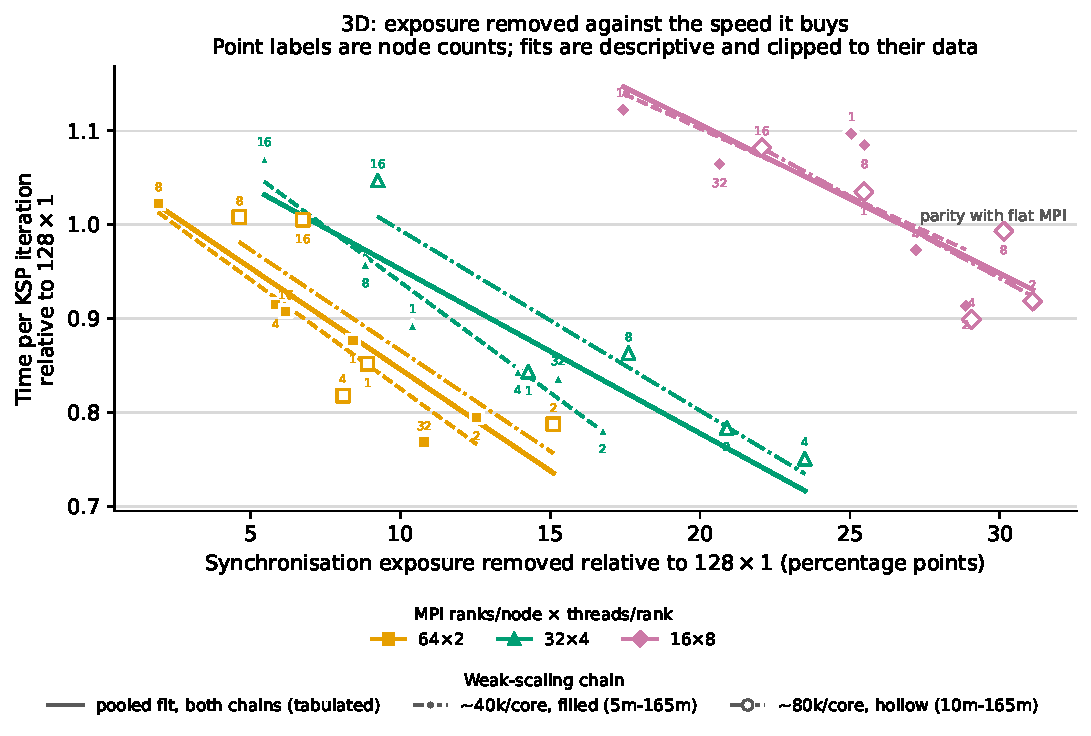
\includegraphics[width=\textwidth]{ksp3d_exposure_tradeoff_by_chain}
  \caption{3D exposure removed relative to flat MPI against the resulting time per
  iteration. Colour is the layout and point labels are node counts. The solid line is the
  pooled fit over all 11 points, the one \Cref{tab:sync-breakeven} tabulates. The two broken
  lines split those points into their weak-scaling chains, dashed with filled markers for
  $\sim$40k unknowns/core and dash-dotted with hollow markers for $\sim$80k. In 3D the three
  stay together, every layout's per-chain break-evens falling within 2.4 points of its pooled
  value. Each line is clipped to the range it was fitted to, so none is extrapolated. The
  fits are descriptive, not predictive.}
  \label{fig:3d-tradeoff}
\end{figure}

\begin{figure}[htbp]
  \centering
  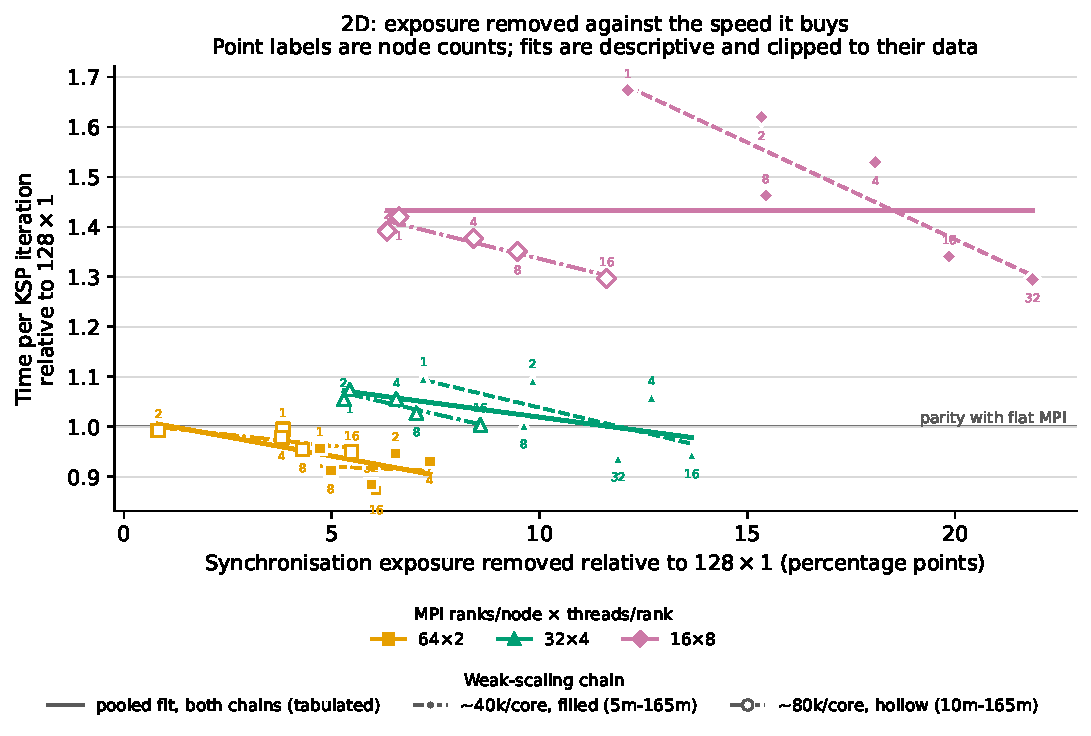
\includegraphics[width=\textwidth]{ksp2d_exposure_tradeoff_by_chain}
  \caption{2D exposure removed relative to flat MPI against the resulting time per
  iteration, styled as in \Cref{fig:3d-tradeoff}. Here the solid pooled fits are not summaries
  of their parts. For $16\times8$ the solid line lies flat while its two chains, correlating
  at $-0.91$ and $-0.96$ separately, descend steeply across it. $64\times2$ and $32\times4$
  depart from their pooled fits as well. Note also that $16\times8$ lies above parity at every
  one of its 11 points, which is read off the markers and not off any fit.}
  \label{fig:2d-tradeoff}
\end{figure}

The relationship between $\mathrm{ExposureRemoved}$ and $\mathrm{TimeRatio}$ accounts
descriptively for two patterns left by \Cref{ch:multinode}. For the first,
holding a 3D layout and chain fixed while increasing the node count makes
$\mathrm{ExposureRemoved}$ and $\mathrm{TimeRatio}$ reverse together at every
step. Along the $\sim$40k chain
in 3D, $32\times4$ has an $\mathrm{ExposureRemoved}$ of 10.4, 16.8, 13.9, 8.8, 5.5 and 15.3
points from one node to 32, and a $\mathrm{TimeRatio}$ of 0.893, 0.781, 0.844, 0.958, 1.070
and 0.837: five transitions, five reversals, including the recovery at 32 nodes where a
9.8-point rise in $\mathrm{ExposureRemoved}$ turns a 7.0\% loss into a 16.3\% gain. All 18
transitions of $64\times2$ and $32\times4$ across both 3D chains behave this way. The
advantage therefore tracks the non-monotone $\mathrm{ExposureRemoved}$ within these
measurements. This concerns the difference, not either share: along this
chain $32\times4$'s own exposure rises monotonically from 34.6\% to 69.3\% and flat MPI's
from 45.0\% to 84.6\%, as \Cref{sec:sync-halo} requires, and only the gap between them turns.

The second is the threshold itself. In 2D, $32\times4$ brackets its own 11.7-point
break-even along the $\sim$40k chain: an $\mathrm{ExposureRemoved}$ of 9.6 points at 41m on
eight nodes for a $\mathrm{TimeRatio}$ of 1.003, then 13.7 points at 82m on 16 nodes for
0.944, crossing parity where the fit puts it. Along the $\sim$80k chain its
$\mathrm{ExposureRemoved}$ never exceeds 8.6 points and it never crosses, bottoming at
1.004. The threshold holds in both directions.

The 2D $16\times8$ row is the counter-example, and \Cref{fig:2d-tradeoff} shows what it
consists of: its pooled $a$ is positive, so the solid line lies flat and the table returns no
break-even at all, while the two broken lines through the very same 11 points, one per chain,
both descend steeply across it. The flatness is therefore an artefact of pooling. Taken
separately the chains correlate at $-0.91$ over the six $\sim$40k points and $-0.96$ over the
five $\sim$80k points, among the tightest fits in the study. What the layout lacks is
therefore not a relationship between $\mathrm{ExposureRemoved}$ and speed but enough of the
former: each chain's line reaches parity only beyond the largest $\mathrm{ExposureRemoved}$
the layout ever attains, 21.9 points, so neither threshold can be stated without
extrapolating and neither is ever reached. That it is slower than flat MPI by 29--67\% at every one of its 11 points is
a direct observation and needs no fit. Some other cost dominates. 

\Cref{tab:map-shares} identifies that cost: 
at the same problem size and node counts, $16\times8$ spends more of its core-time
waiting in the OpenMP runtime than any other layout, 76.5\% against 48.3\% for
$64\times2$ at eight nodes. The two halves of the trade are therefore both measured, one
on the full matrix without a profiler and the other on eleven profiled cells with one.
What remains unmeasured is their sum: the profiled and unprofiled quantities come from
different instruments on different runs and cannot be added into a single budget.

\subsection{What This Does and Does Not Establish}
\label{sec:sync-limits}
Pooling all 33 hybrid measurements of a dimension breaks the relationship between
$\mathrm{ExposureRemoved}$ and $\mathrm{TimeRatio}$, and breaks it differently in each
dimension. In 2D the pooled correlation is $+0.58$, where the two layouts that
have a break-even give $-0.67$ and $-0.59$. In 3D it falls to $+0.10$ from three values that
all exceed $0.8$ in magnitude.

The first candidate is $16\times8$, which has the largest $\mathrm{ExposureRemoved}$ and is
also the slowest. That is enough in 3D: drop it and the pooled figure returns to $-0.75$. It is
not enough in 2D, where dropping it still leaves $+0.13$. There, $32\times4$ has a larger
$\mathrm{ExposureRemoved}$ than $64\times2$ at all 11 points and is slower at all 11. The ordering between layouts runs
against the ordering within them in both dimensions, and $16\times8$ is only the most
extreme case of it. The relationship holds within a layout, so a pooled figure would mislead.

The two weak-scaling chains cannot be pooled either, and that is a second and
independent effect: in 3D it does little harm, every layout's per-chain break-evens
falling within 2.4 points of its pooled one, while in 2D none of the three layouts
survives unchanged and $16\times8$ inverts the sign. \Cref{tab:sync-breakeven} still
reports pooled fits, because five and six points are too few to fit a chain on its
own, and its columns should be read with that in mind. The $b$ column agrees across
dimensions only because the fits are pooled: split the chains and the agreement
loosens at $32\times4$ and fails on the $\sim$40k chain at $16\times8$. Neither
pooling changes which layouts beat flat MPI, because that is read off the
measurements and not off a fit.

Within PETSc's event accounting, layout advantage tracks lower halo-exchange exposure,
with global reduction secondary. MAP places the opposing sampled cost in OpenMP wait paths.
Neither observation excludes a memory or cache mechanism underneath those software events.
\Cref{sec:rq4} names the candidates, and \Cref{sec:futurework} gives the counter experiment.

% VERIFIED 2026-08-08, sec:sync-limits simplified. Sentences shortened and three paragraphs
%   split into five; no claim dropped. Every number recomputed from
%   repeated_fullnode_exposure_tradeoff.csv, both dimensions, and unchanged:
%   pooled r over all 33 rows = 2D +0.5804, 3D +0.0983; dropping 16x8 (22 rows) = 2D +0.1252,
%   3D -0.7472. -0.67/-0.59 and the three |r|>0.8 are tab:sync-breakeven's r column.
%   CORRECTION: "every layout's per-chain fits bracket its pooled one" was FALSE and is now
%   "every layout's per-chain break-evens fall within 2.4 points of its pooled one", which is
%   the wording fig:3d-tradeoff's caption already used. Per-chain against pooled break-even:
%   3D 64x2 pooled 2.860 in [2.475, 3.746] -- brackets; 3D 32x4 pooled 7.273 BELOW both
%   (7.400, 9.686) -- does not; 3D 16x8 pooled 26.723 below both (26.724, 27.033) by 0.001
%   -- does not. Checked under three readings and 32x4 fails all three: its per-chain slopes
%   (-0.02354, -0.01921) are both steeper than pooled (-0.01747) and its per-chain intercepts
%   (1.1742, 1.1861) both higher than pooled (1.1270). A pooled line through two vertically
%   offset clusters can be flatter than either, which is what happens here. The "at most 2.4
%   points" half was and remains correct: max shift 2.413, at 3D 32x4 on the ~80k chain.
%   NARROWED: "removes more exposure than 64x2 over its whole range while being slower over
%   its whole range" -> "at all 11 points ... slower at all 11". Same fact, now checkable:
%   the claim is POINTWISE at matched scale/nodes and is 11/11 in both directions. It could
%   not be a range claim -- tab:sync-breakeven's printed ranges OVERLAP in both columns
%   (exposure 0.8-7.4 against 5.3-13.7, time 0.872-0.995 against 0.937-1.096), so a reader
%   checking the old wording against the table would have found it apparently false.
%   THINNED, per the P3 split: the positive half (what the data DO show) stays here, which
%   sec:sync-limits owns. The two enumerations that followed were near-verbatim duplicates of
%   sec:rq4 -- same three thread-wait causes in the same order, same four exposure-share
%   confounds in the same order, both opening "Knowing that threads wait does not say" -- and
%   are now a \Cref to it. Nothing is lost: sec:rq4 carries both lists and adds "all predict
%   the same signature", and the dropped "attributing anything to cache capacity" is covered
%   by sec:futurework's "memory-bandwidth and cache-miss counters". The
%   "no hardware mechanism" position still lives here, as CLAUDE.md requires.
% G8 CLOSED 2026-07-31: the placeholder section "Preconditioner Reuse in the Scaling
%   Context" is REMOVED. Its intended content is already stated where it is load-bearing:
%   the motivation and the 69%/93% stage shares in \Cref{sec:whyrepeat}, the reuse options
%   and the zeroed initial guess in \Cref{sec:benchmarks}, and the scope limit it implies
%   ("applies to applications that solve repeatedly with the same operator") in
%   \Cref{sec:threats}. A separate section would only repeat them.

% VERIFIED 2026-08-07 for the pooling paragraph, recomputed from the exposure_tradeoff CSVs
%   as tradeoff.exposure_removed_pt.corr(time_ratio):
%     pooled, all 33 rows      2D +0.5804   3D +0.0983
%     pooled, 16x8 dropped     2D +0.1252   3D -0.7472   (22 rows)
%   CORRECTION: the paragraph used to say pooling "inverts the sign ... per dimension" and
%   quoted only the 2D figure. Both halves were wrong to generalise. 3D does flip sign but
%   to +0.10, which is destruction of the correlation, not inversion; and the stated cause
%   ("because 16x8 combines the largest exposure reduction with the worst performance") is
%   sufficient ONLY in 3D, where removing 16x8 restores -0.75. In 2D removing it leaves
%   +0.13, still positive, because 32x4's exposure-removed range (5.3-13.7) sits ABOVE
%   64x2's (0.8-7.4) while its time-ratio range (0.937-1.096) also sits above 64x2's
%   (0.872-0.995) -- both readable off tab:sync-breakeven. So the between-layout ordering
%   opposes the within-layout one for every pair in 2D, and 16x8 is the extreme case rather
%   than the whole cause. Do not restore the single-cause wording.
%   NOT ADDED, needs a check first: tab:map-shares' MPI core-time share has a structural
%   ceiling of 1/(threads per rank) if MPI is only ever called from the master thread --
%   50%, 25%, 12.5% for 64x2/32x4/16x8, against measured 46.7/22.6/6.2 at eight nodes. If
%   that holds, the cross-layout MPI ordering in sec:map-matrix is partly arithmetic and the
%   phrase "reproduced here by a different instrument on a different quantity" overstates
%   the independence. The OpenMP column has the mirror-image ceiling, (t-1)/t = 50/75/87.5%
%   against measured 48.3/69.3/76.5%. sec:map-matrix's FIXED-LAYOUT observation (16x8 from
%   53.5% to 76.5% between two and eight nodes) is unaffected, since the ceiling is constant
%   there, which is why that one is called the discriminating observation. Before writing
%   any of this down, confirm from the build or a log that PETSc issues MPI outside its
%   OpenMP regions (MPI_THREAD_FUNNELED, not MULTIPLE); the numbers are consistent with it
%   but consistency is not proof.
% VERIFIED 2026-08-07: SECOND pooling axis found -- the weak-scaling CHAINS, independent of
%   the layout pooling above. np.polyfit per layout per chain (40k n=6, 80k n=5) against the
%   pooled n=11 row of tab:sync-breakeven, from the exposure_tradeoff CSVs:
%     3D 64x2  r -0.97 / -0.80 vs pooled -0.86 ; BE 2.5 / 3.7 vs 2.9
%     3D 32x4  r -0.98 / -0.93 vs pooled -0.90 ; BE 7.4 / 9.7 vs 7.3
%     3D 16x8  r -0.76 / -0.85 vs pooled -0.83 ; BE 27.0 / 26.7 vs 26.7
%     2D 64x2  r -0.08 / -0.73 vs pooled -0.67 ; 40k chain has essentially NO relationship
%     2D 32x4  r -0.66 / -0.92 vs pooled -0.59 ; BE 11.9 / 8.8 vs 11.7
%     2D 16x8  r -0.91 / -0.96 vs pooled +0.00 ; SIMPSON'S PARADOX
%   "at most 2.4 points" is 3D 32x4, 9.7 against a pooled 7.3; the other two move 0.8 and 0.3.
%   2D 16x8 is the serious one. Its two chains are steep lines with very different intercepts
%   (b = 2.1510 on 40k, 1.5427 on 80k); superposed they read as a flat cloud, which is what
%   fig:2d-tradeoff shows and what the old text called "exposure removal predicts nothing
%   there". That reading was WRONG -- within each chain this layout has among the tightest
%   fits in the study. The real obstacle is that both chains reach parity at 29.7 and 26.2
%   points while the layout never removes more than 21.9.
%   THOSE TWO BREAK-EVENS ARE NOT PRINTED, deliberately: both exceed the observed range, so
%   quoting them would violate this section's own "no break-even figure is an extrapolation".
%   The text states only the non-extrapolated part (the two correlations) and then falls back
%   on the direct measurement, time ratio 1.294-1.674 at every one of the 11 points.
%   The section's CONCLUSION is unaffected: 2D 16x8 is slower than flat MPI everywhere either
%   way. What changed is the reason given for it.
%   NOT FIXED, needs your call: the paragraph after tab:sync-breakeven reads the b column
%   across dimensions as "1.1305 against 1.1270 and 1.4313 against 1.4226". Per chain the
%   32x4 pair survives but loosens (b-1 is 0.236 vs 0.174 on 40k, 0.169 vs 0.186 on 80k,
%   against 0.131 vs 0.127 pooled), while the 16x8 pair holds only on 80k (1.5427 vs 1.4670)
%   and fails badly on 40k (2.1510 vs 1.3929). sec:sync-limits now says this in one clause;
%   whether that paragraph should also be weakened is an editorial decision, not a numbers one.
% VERIFIED 2026-08-07: fig:2d-tradeoff and fig:3d-tradeoff REPLACED. They were
%   ksp{2,3}d_exposure_tradeoff, from analyze_event_breakdown.py's make_tradeoff_plot, which
%   drew all 11 points of a layout in one colour with one marker and one POOLED fitted line.
%   Two defects: the chains were indistinguishable, so no point the text names could be
%   located; and the pooled line is the only thing drawn, so the 2D 16x8 Simpson effect was
%   invisible -- the figure showed the artefact and hid the parts that produce it.
%   Now ksp{2,3}d_exposure_tradeoff_by_chain, from the new
%   analysis/scripts/nproc_2d_libsci/plot_exposure_tradeoff_by_chain.py, which panels by
%   chain, labels every point with its node count, draws each chain's own fit solid and
%   repeats the pooled fit dotted in both panels. The 2D 16x8 contrast is now the most
%   visible thing in that figure: one flat dotted line across two steeply descending solid
%   ones. The script reads ONLY repeated_fullnode_exposure_tradeoff.csv, so it runs without
%   the raw logs, the same arrangement as plot_sync_share_by_chain.py; its colours, markers,
%   CHAINS mapping, panel layout and legend are copied from that script so the Chapter 5
%   trade-off figures read like the Chapter 4 scaling ones. Its --report output reproduced
%   the per-chain fits above independently.
%   Each fitted line is clipped to the range it was fitted to. Spanning the panel instead
%   sent 2D 16x8's 40k line to 2.15 at zero exposure removed, twelve points left of its
%   leftmost measurement, which contradicts this section's own no-extrapolation rule.
%   Chain membership is matched on the (nodes, scale) pairs of CHAINS, not by thresholding
%   unknowns_per_core, so it is the same mapping the Chapter 4 figures use; the loader raises
%   if any of the 33 points matches neither chain.
%   The old figures are left in figures/ and are no longer included by draft.tex.
% VERIFIED 2026-08-07, second pass on the replacement figures. Both dimensions are now ONE
%   axes, not two panels: a layout is one colour and one marker shape, the ~40k chain is
%   filled/dashed and the ~80k chain is hollow/dash-dotted. SOLID IS RESERVED FOR THE POOLED
%   FIT, so the line a reader traces from tab:sync-breakeven is the prominent one and the two
%   chains are visibly the things departing from it. In 2D 16x8 that is a flat solid line with
%   two steeply descending broken lines crossing it, which is the artefact and its cause in
%   one picture.
%   FOUR prose repairs the new figures forced, all because the old text described the OLD
%   figure and the new one contradicts it:
%   (a) The b-column sentence dropped the 16x8 pair. 1.4313 against 1.4226 is a pooled-fit
%       coincidence: per chain it is 2.1510 vs 1.3929 on 40k, which fails by 0.76, and only
%       1.5427 vs 1.4670 on 80k. The 32x4 pair survives separation (b-1 = 0.236 vs 0.174 on
%       40k, 0.169 vs 0.186 on 80k) so it is kept, now scoped and pointed at sec:sync-limits.
%       "Only 64x2 differs appreciably" went with it: with 16x8 removed the sentence covers
%       one layout, so a claim about which others differ has nothing left to rank.
%   (b) "Neither figure can show it, because both discard node count" was TRUE of the old
%       figures and is now FALSE -- every point carries its node count. DO NOT RESTORE IT.
%       The replacement states the method instead of arguing about what the figure can show:
%       hold a layout and a chain fixed, walk the node count, and the two quantities reverse
%       together. An intermediate version explained that no fitted LINE can show it (they are
%       monotone by construction and the x axis is exposure removed) while the point LABELS
%       can; that was accurate but was meta-commentary on figure-reading, and the plain
%       statement of method makes it unnecessary. The walk remains traceable on the figure
%       via the node labels, which the caption already says.
%   (c) "shows it as a flat cloud among two descending lines" described the pooled scatter.
%       There is no cloud now; it is a flat solid line with two descending broken ones.
%   (d) The figure lead-in gained one sentence naming the filled/hollow and solid/broken
%       encoding, since the reader meets it before either caption.
%   Numbers unchanged throughout: -0.91, -0.96, the 10.4/16.8/13.9/8.8/5.5/15.3 walk, the
%   18 transitions, 9.6/13.7 against 11.7, and the 8.6/1.004 ceiling on the 2D 80k chain.

% ===== FILE: chapters/ch7_discussion.tex =====
\chapter{Discussion}
\label{ch:discussion}
% Write once results are final. Outline: 00 §Ch7.

\section{Answering the Research Questions}
\label{sec:rqs}
The four questions of \Cref{sec:aims} are answered in turn. RQ1 and RQ2 rest on
\Cref{ch:multinode}, RQ3 on \Cref{ch:profiling}, and RQ4 on the limits of both.

\subsection{RQ1: Does the threaded backend reduce time to solution, and by how much?}
\label{sec:rq1}
Yes. Hybrid execution cuts steady-state solve time in both dimensions. What differs
between 2D and 3D is how the gain behaves as the job grows, not whether there is one.

In 2D the gain grows with node count. Along both unknowns/core chains, every hybrid layout
gains on flat MPI as the node count grows, and four of the six series gain at every step.
$64\times2$ is faster per iteration than flat MPI at all 11 size--node points, and its
margin widens from 4.3\% at one node to 12.8\% at 16. $32\times4$ starts 9.6\% slower at
one node and ends 6.3\% faster at 32. A layout comparison made on one or two nodes
therefore does not predict what happens on 16 or 32, which is the practical content of the
2D result.

In 3D the gain is larger but follows no such trend. The best hybrid gain in throughput is
33.2\%, against 14.7\% in 2D, and two-thirds of the hybrid points are faster per iteration
than flat MPI. No series gains at every step. The advantage is largest at two to four
nodes, is gone by eight to 16, and returns at the largest point. On raw throughput
$32\times4$ wins six of the 11 points, $64\times2$ four, and flat MPI one. In 3D the best
balance depends on both problem size and node count, which the 2D data do not show.

\subsection{RQ2: At which balance, and how does the answer change with the regime?}
\label{sec:rq2}
At constant work per core the useful range is two to four threads per rank in both
dimensions. Which of the two is better depends on the dimension: $64\times2$ everywhere in
2D, and either $32\times4$ or $64\times2$ in 3D depending on size and node count.

Holding the problem size fixed does not change which layouts are good at moderate scale. It
changes what the choice costs, from a few per cent to whole factors, because the layouts
differ in where they stop scaling. In 2D none of them stops. On 20.25M unknowns the four
stay within a factor of 1.81 of each other from one node to 32, and all four are still
getting faster at the end, the last doubling worth 1.11 to $1.39\times$. In 3D they come
apart. On the matched 20.35M problem flat MPI stops improving after eight nodes,
$64\times2$ and $32\times4$ after 16, and only $16\times8$ is still improving at 32. Flat
MPI ends $2.6\times$ slower at 32 nodes than at its own best point, so at 4096 cores the gap
to $16\times8$ reaches $3.81\times$.

Eight threads per rank does not run faster at a given scale. It keeps improving at a scale
where the others have stopped. That is the whole case for it. $16\times8$ wins no
raw-throughput point in either weak-scaling campaign, and its good weak-scaling efficiency
in 2D is not a point in its favour either, for the reason given in \Cref{sec:threats}. Where
it does earn its place is the fixed-size curves of \Cref{sec:strong20m}. Drive the problem
down to about 4.9 thousand unknowns per core, far below the 25--100 thousand the admission
window of \Cref{sec:configspace} allows, and $16\times8$ is the fastest 3D layout at 32
nodes and the only one of the four still improving. Flat MPI has by then been getting slower
for two doublings, which is where the $3.81\times$ above comes from.

A layout recommendation means nothing without the scaling regime it was measured in. The
same eleven size--node pairs, read at constant work per core, put the useful range at two to
four threads and rank $16\times8$ last. The same solver and build on a fixed problem make
$16\times8$ the only 3D layout still improving at 4096 cores.

Both throughput views are needed. Raw throughput is the time this solver configuration
actually pays, and it includes any change in GAMG convergence. Time per iteration takes the
iteration count out by holding the outer KSP count fixed, but even that does not make the
GAMG hierarchy or the communication volume the same across decompositions.

\subsection{RQ3: Which parts of the solve account for the difference?}
\label{sec:rq3}
\Cref{sec:bottleneck} shows that hybrid layouts spend less time exposed to halo exchange and
global reductions than flat MPI, at all 22 size--node points, and halo exchange is the larger
of the two. Within one layout, how much exposure it removes tracks how much faster it is
($|r|$ up to $0.90$). Layouts with more threads per rank have to remove more exposure before
they break even. This is consistent with the useful two-to-four-thread range and the uneven
3D ordering, but does not establish their cause.

The other half of that trade is measured too, on eleven Linaro MAP profiles of the 20.25M
2D problem. Within the solve window the share of core-time spent waiting in the OpenMP
runtime rises with threads per rank (48.3\%, 69.3\% and 76.5\% at eight nodes) while the
MPI share falls (46.7\%, 22.6\% and 6.2\%). Both orderings hold on two different PETSc
builds. What hybrid execution saves in MPI it gives back, in part, as threads waiting on
each other. Those samples are consistent with the poor 2D $16\times8$ result, but do not
exclude a cache, bandwidth or imbalance mechanism. \Cref{sec:rq4} sets that boundary.

\subsection{RQ4: How far do the trends generalise, and what would establish a mechanism?}
\label{sec:rq4}
These measurements say what happens. They do not say what is happening in the hardware
underneath, and that is the level left open. Knowing that threads wait does not say what
they are waiting for. Three causes fit the data equally well: PETSc threads only part of
its solve path, the threaded regions may be too short to pay back the cost of a barrier,
and memory bandwidth may already be saturated. All three would look the same here. The
exposure share has the same problem. It cannot separate message latency, bandwidth, cost
that grows with the number of ranks, and imbalance elsewhere in the iteration. The profiled
and unprofiled quantities also come from different instruments, so they cannot be added into
one time budget. No hardware mechanism is established here.

How far the trends generalise is bounded by the scope set out in \Cref{sec:threats}: two
structured-grid Poisson problems, one PETSc version and compiler environment, one CG+GAMG
configuration, solves that reuse a fixed operator, and PETSc's default row decomposition.
Within that scope the patterns hold across two dimensionalities, six problem sizes and two
scaling regimes, and the exposure and OpenMP-wait orderings that go with them reproduce on a
second PETSc build. The 2D and 3D campaigns are not two independent checks, though. Both use
the same row decomposition, and that decomposition is also what makes them differ.
\Cref{sec:futurework} lists what would extend them: hardware counters for the mechanism, a
second and third fixed problem size for the saturation ordering, and node counts beyond 32
to find the turning points this campaign brackets only from below.

% PLAIN-LANGUAGE PASS 2026-08-09, sec:rqs. WORDING ONLY. No number, hedge or claim scope
%   was touched, so the 2026-08-08 verification below still stands in full. What changed:
%   "the shape of the result, not which layout wins" -> "how the gain behaves as the job
%   grows, not whether there is one"; "the answer is ordered" / "larger but unordered" ->
%   "the gain grows with node count" / "larger but follows no such trend"; "a term that does
%   not grow with concurrency already dominates its per-iteration cost" -> "part of its
%   per-iteration cost does not grow when cores are added, and that part is already the
%   larger one"; "buys a later saturation limit, not a better operating point" -> two plain
%   sentences; "At the event-accounting level, the opposing cost appears in OpenMP wait
%   paths" -> "What hybrid execution saves in MPI it gives back, in part, as threads waiting
%   on each other"; "What remains unexplained is one level lower" -> "These measurements say
%   what happens. They do not say what is happening in the hardware underneath"; "all predict
%   the same signature" -> "all three would look the same here"; "rank-count-dependent
%   metadata" -> "cost that grows with the number of ranks"; "not independent of the last
%   item: they share a decomposition, and it is what sets them apart" -> "not two independent
%   checks ... the same row decomposition ... is also what makes them differ".
%   "admission window" is KEPT (it is sec:configspace's defined term, also used at
%   sec:strongdesign and sec:threats) but now carries its 25-100k unknowns/core gloss inline.
%   Two semicolons joining independent clauses were split into full stops, per the house
%   style rule; the RQ1 "Yes." opener is deliberate.
% REORDERED 2026-08-09, the RQ2 fixed-size paragraph. It ran data-then-conclusion and buried
%   the point in its last two sentences. Now conclusion first, in the opening two sentences,
%   then 2D and then 3D as evidence for it. No number changed and none was dropped: 20.25M,
%   1.81, "from one node to 32", 1.11-1.39x, 20.35M, 8/16/32, 2.6x, 4096 cores, 3.81x all
%   survive. "from one node to 32" is still load-bearing, see the 2026-08-08 note below:
%   1.81 is the spread at 16 nodes, the largest over the six node counts, not the 32-node
%   one, which is 1.476. "Three layouts stop improving and start getting slower" was dropped
%   as a count and the three are simply named, which is shorter and says the same thing.
%   "$16\times8$ has not turned by 32" -> "only $16\times8$ is still improving at 32":
%   same fact, and it no longer leans on Ch4's "turns upward", which this chapter had
%   otherwise stopped using.
% REORDERED 2026-08-09, the three remaining RQ2 paragraphs, same treatment. Each now opens
%   with its conclusion and follows with the evidence:
%   (a) the 16x8 paragraph opens on "Eight threads per rank does not run faster at a given
%       scale", which was its last two sentences, and the wins-nothing / best-efficiency
%       pair is then introduced as the two results that follow from it. "On its own that
%       says more about the metric than about the layout" became "The efficiency figure is
%       the weaker of the two", said before the explanation instead of after it. The
%       trailing "It is 3.81x faster there than flat MPI" was DROPPED as a restatement: the
%       preceding paragraph now ends on that same 3.81x, so the sentence pointed at a number
%       two lines above it. Replaced by "which is where the 3.81x above comes from", which
%       ties the two paragraphs together instead of repeating the measurement.
%   (b) "That contrast is also a result about method" was a pure throat-clearing lead-in and
%       is gone. The paragraph now opens on the claim itself, "A layout recommendation means
%       nothing without the scaling regime it was measured in", formerly its last sentence.
%   (c) the metrics paragraph opens on "Both throughput views are needed", formerly its last
%       sentence, then says what each view is and what it does not fix.
%   No number changed: 25-100 thousand, 4.9 thousand, 32 nodes, 3.81x, two to four threads,
%   4096 cores all survive. The hedges survive too, and one is now earlier and harder to
%   miss: "even that does not make the GAMG hierarchy or the communication volume the same
%   across decompositions" still limits what time per iteration is allowed to prove.
% CUT 2026-08-09, on request, from the 16x8 paragraph: the three sentences explaining WHY
%   weak-scaling efficiency flatters this layout ("it compares a layout only against its own
%   baseline ... part of its per-iteration cost does not grow when cores are added, and that
%   part is already the larger one"). Now a single clause pointing at \Cref{sec:threats}.
%   CHECKED BEFORE CUTTING, three ways, because a dropped caveat is the dangerous kind of
%   edit: (a) nothing anywhere \Cref's sec:rq2, so no section was relying on the argument
%   being made here; (b) the caveat itself survives in THREE other places, none of them
%   touched -- tab:weak-eff's caption ("Each layout is measured against itself, so this
%   quantifies degradation, not absolute speed"), sec:weak-ranking ("A metric based on each
%   layout's own baseline can reward a poor baseline"), and sec:threats, which states it in
%   full and adds "never on its own"; (c) sec:guidance already routes the reader to
%   sec:threats for exactly this point, not to sec:rq2, so the pointer added here matches an
%   existing convention rather than inventing one.
%   The only thing genuinely lost is the mechanism sentence, that a concurrency-independent
%   term already dominates 16x8's per-iteration cost. That was an EXPLANATION, not a
%   measurement, and it appeared nowhere else, so nothing downstream cites it. The house
%   "say it once" rule was on the side of the cut: sec:threats owns this caveat.
%   Also plainer in the same edit: "Pushed below the 25--100 thousand unknowns per core that
%   the admission window ... allows, down to about 4.9 thousand per core" -> "Drive the
%   problem down to about 4.9 thousand unknowns per core, far below the 25--100 thousand the
%   admission window ... allows". Both numbers kept, imperative instead of two stacked
%   participles.
% CONDENSED 2026-08-09, sec:threats, on request: state the threat, then one short
%   consequence. About 640 words to about 470, six paragraphs still six.
%   NO THREAT WAS DROPPED, and that was checked first: every one of the six paragraphs is
%   the target of a \Cref from somewhere else, so this section cannot be thinned by deletion.
%   The nine inbound references and what each needs to still find here:
%     sec:contributions  "what the retained evidence cannot establish"  -> the whole section
%     sec:benchmarks     "what this scopes the results to"              -> P2, decomposition
%     sec:superseded     "restates the limit"                           -> P5, rtol defect
%     sec:map-matrix     "could previously only state as a limit"       -> P6, LibSci
%     sec:rq2, sec:guidance  "for the reason given in sec:threats"      -> P4, weak efficiency
%     sec:rq4            "the scope set out in sec:threats: ..."        -> P1, the scope list
%     sec:conclusions    "sec:threats shows makes the halo large"       -> P2
%     sec:futurework     "the 3D halo of sec:threats"                   -> P2
%   P4 is UNCHANGED, word for word. Three sections now route the weak-scaling-efficiency
%   caveat here, including sec:rq2 since today's cut, so it is the one paragraph that must
%   read exactly as the sections pointing at it assume.
%   P1 gained "and solves that reuse a fixed operator" so the scope list here matches the
%   five-item list sec:rq4 quotes; previously rq4 named an item this section only implied.
%   Numbers kept: 69%, 2.03L/0.64L/0.18L/0.02L, 48 points, 11.1%, 9-13 and 6-7 iterations,
%   2.4e-10 at 6400^2, 2.1%, 164.56 million, 32 nodes.
%   Dropped as restatement, not as claim: "That makes the halo larger, and the halo is what
%   the whole of Ch5 measures" (the next sentence gives the halo figures, which show it);
%   "the chains and the doublings describe one campaign of 11 size--node pairs" (sec:bands
%   and sec:strong20m both say it); "its 32-node point sits outside the admission window by
%   design" (sec:strong20m states it where the campaign is defined, and sec:rq2 repeats the
%   4.9-thousand figure); "The exploratory campaigns therefore differ from the production
%   ones in both solver and tolerance" (the two preceding clauses are those two differences).
% CONDENSED 2026-08-09, sec:guidance, same treatment. About 330 words to about 250, four
%   paragraphs still four. Nothing \Cref's this section, so unlike sec:threats it had no
%   inbound contract to honour; the constraint here was simply not to drop a recommendation.
%   All four survive: 64x2 in 2D, test both in 3D, do not default to 16x8, and choose for
%   the regime. Rewritten as instructions rather than descriptions of what was measured,
%   since this is the one section of the dissertation the reader is meant to act on:
%   "For this repeated 2D CG+GAMG workload, 64x2 is the best default among the tested
%   full-node layouts" -> "In 2D, default to 64x2"; "Small one-node jobs should still test
%   flat MPI, which gives ..." and "Jobs above roughly eight nodes should also test 32x4"
%   merged into one "Two things are still worth a test" sentence carrying both exceptions.
%   Numbers kept: 4.3/12.8, 5.9/9.5 at 5m/10m, 33.2 at 41m/4n, 30.1 at 165m/32n, the 80k
%   16-node exception, 4.9 thousand per core at 32 nodes, 25 thousand.
%   Dropped as restatement: "while flat MPI had been getting slower for two doublings and
%   both intermediate layouts for one" (sec:rq2 and sec:conclusions both carry the turning
%   points, and "the only one of the four still improving" already implies the other three).
%   "comfortable occupancy" -> "comfortable work per core" in the last sentence: occupancy
%   means node population everywhere else in this document, and every layout here is fully
%   populated, so the word was pointing at the wrong quantity.
% VERIFIED 2026-08-08, sec:rqs simplified. Shorter sentences, plainer words, three long
%   sentences split; no claim dropped. Every number rechecked and unchanged:
%   RQ1 "four of the six series" and RQ1 3D "no series" = cross_dimension_summary.csv
%   monotone_ratio_series 4/6 and 0/6. 64x2 faster at all 11 2D points: 11/11 from
%   repeated_fullnode_exposure_tradeoff.csv. 4.3->12.8 and 9.6->6.3 are the ~40k chain
%   (5m/1n 0.9568, 82m/16n 0.8719; 5m/1n 1.0962, 165m/32n 0.9370); on the ~80k chain the
%   one-node margin is only 0.5%, so the chain is doing work in that sentence.
%   33.2/14.7 = best_throughput_gain (3D 32x4 41m/4n, 2D 64x2 82m/16n); "two-thirds" =
%   hybrid_faster_per_iteration 22 of 33, exactly 2/3. RQ2 1.81 = the LARGEST spread over
%   the six node counts, at 16 nodes (0.0568/0.0313 = 1.815), not the 32-node one (1.476) --
%   "from one node to 32" is load-bearing, do not trim it. 2.6x = 0.2599/0.0997 = 2.607 and
%   3.81x = 0.2599/0.0681 = 3.816, both off tab:strong20m-grid-3d. Turning points 8/16/16/>32
%   are that grid's per-row minima. 16x8 wins 0 of 11 2D throughput points (64x2 8, 128x1 3).
%   CLARIFIED, not changed: "the best hybrid margin is 33.2%" -> "the best hybrid gain in
%   throughput", and "two-thirds ... are faster" -> "faster per iteration". The two adjacent
%   RQ1 paragraphs quote DIFFERENT metrics -- 4.3/12.8/9.6/6.3 are per-iteration margins,
%   33.2/14.7 are throughput gains -- and only RQ2's last paragraph said so. Now each number
%   carries its own metric.
%   CORRECTION: "reduces the share ... at 21 of the 22 size--node points" -> "at every one of
%   the 22". It is 22/22: all three hybrid layouts have exposure_removed_pt > 0 at 11/11
%   points in each dimension, and analyze_event_breakdown.py line 398 RAISES on <= 0, so
%   22/22 is structural. The 21/22 belongs to a different claim, sec:sync-halo's strict
%   four-layout ordering by MPI rank count, which is 2D 11/11 and 3D 10/11 -- the exception
%   being 3D 82m/16n, where 64x2 (68.6) sits below 32x4 (69.3). This is the SECOND time that
%   borrowing has been caught: the % VERIFIED note at sec:sync-breakeven records the same
%   number leaking into "nearly every point" there and being corrected on 2026-08-06. The
%   fix was applied there and missed here. Like that one, it makes the claim STRONGER.
%   NOT VERIFIABLE from the repo: RQ1's 3D throughput split "six / four / one". Only the
%   six is recorded (cross_dimension_summary.csv throughput_wins_top_count for 32x4); there
%   is no repeated_fullnode_best_layouts.csv under nproc_3d_libsci/tables/, so the four and
%   the one cannot be re-derived. Their sum checks out (6+4+1 = 11). Needs the raw logs.
%   SUPERSEDED 2026-08-09: it IS verifiable, from weak_scaling_best_layouts.csv under the
%   2D tree, which carries both dimensions. All three counts confirmed. See the note at the
%   end of sec:futurework for the row-by-row derivation. No raw logs needed.
\section{Threats to Validity}
\label{sec:threats}
The matrix covers two structured-grid Poisson problems, one PETSc version and compiler
environment, one CG+GAMG configuration, and solves that reuse a fixed operator. Nothing
here need transfer to unstructured matrices, other preconditioners, or solver phases that
call dense BLAS. The reuse is the limit that bites hardest: setup was a median 69\% of
measured time in the single-solve campaign of \Cref{sec:superseded}, which ranked the
layouts differently. An application dominated by one-off solves should expect that ranking,
not this one.

The largest limit is the decomposition. Both drivers take PETSc's default contiguous row
blocks, so a subdomain is a slab and not a cube, and the halo follows the $\min(L,\,mn)$
form of \Cref{sec:benchmarks} rather than the $N^{2/3}$ of a Cartesian decomposition. At
164.56 million unknowns on 32 nodes that gives flat MPI a halo of $2.03L$ in 3D and $0.64L$
in 2D, against about $0.18L$ and $0.02L$ for cube-shaped subdomains. The layout comparison
survives this, because all four layouts run the same code and the model reproduces their
measured ordering at all 48 points checked. The explanation does not: hybridisation reduces
exposure to a halo that this decomposition makes large, and a \texttt{DMDA} driver would
start from a much smaller one. \Cref{sec:futurework} names the run that would settle how
much of the advantage remains.

Three repeats give an observed range, not a significance test. The unknowns-per-core filter
allows at most two node counts per problem size, so every strong-scaling step inside the
formal matrix covers one doubling, and reading the same points as two weak-scaling chains
lengthens the curves without adding measurements. The fixed-size extension supplies genuine
six-point curves, but at one problem size per dimension, so whether the 3D saturation
ordering holds at other sizes is untested. Its spreads are also larger, up to 11.1\%,
because the per-solve time at 32 nodes is only tens of milliseconds.

Weak-scaling efficiency is computed against each layout's own single-node time, so it
measures degradation and not speed, and it rewards a layout whose baseline is poor. It
must be read together with \Cref{fig:2d-ratio} and \Cref{fig:3d-ratio}, never on its own.

Dividing by the iteration count removes the 9--13 iterations in 2D and 6--7 in 3D, but not
the GAMG work that changes with the decomposition inside an iteration. The single-node
configuration-space sweep is weaker still. It used the default rank-dependent block-Jacobi
solver, and its double-dashed \texttt{-{}-ksp\_rtol 1e-5} was never consumed by PETSc
(\Cref{sec:solver}), so those runs converged against a mesh-dependent tolerance reaching
$2.4\times10^{-10}$ at $6400^2$. It therefore sets the search bound and nothing more. No
default-versus-GAMG comparison is drawn from it, and the conclusions that do rest on it
hold at a fixed rank count or per iteration, where the tolerance is common to the runs
being compared. All formal runs pass the option with a single dash.

The formal runs link threaded LibSci, but \Cref{sec:map-matrix} shows the repeated sparse
solve barely calls it, at most 2.1\% of solve-window core-time, so it is ruled out as an
explanation rather than left unproven. MAP timings stay out of the scaling curves because
profiler overhead is large and uneven, and for the same reason the profile shares are read
as an ordering between layouts and not as absolute costs. There is one profile per cell and
none at $128\times1$. Hardware-mechanism claims remain outside the evidence established
here.

% ===== FILE: chapters/ch8_conclusion.tex =====
\chapter{Conclusion and Future Work}
\label{ch:conclusion}

\section{Conclusions}
\label{sec:conclusions}
The corrected 2D and 3D campaigns contain 264 formal runs across 88 configurations from one
to 32 ARCHER2 nodes, and the matched fixed-size extension adds 144 more across 48. Sixteen
pilot logs are kept for the record but excluded from the statistics. Every formal run does one
warm-up solve and 19 timed solves with the GAMG hierarchy reused, and every one was validated
against the build, layout, convergence and library PETSc itself reports.

At constant work per core, two to four threads per rank is the reliable range in both
dimensions, and eight threads per rank is not competitive in either. Past that point, 2D and
3D behave differently.

In 2D the layout effect grows with the node count. Every hybrid layout improves relative to
flat MPI as nodes are added, and does so at every step in four of the six layout-and-chain
series. $64\times2$ is faster per iteration than flat MPI at all 11 size--node points, by
4.3\% at one node and 12.8\% at 16, and at 164.56M unknowns on 32 nodes it reaches 794.8
million equations per second, 13.1\% above flat MPI on raw throughput. $32\times4$ starts
9.6\% slower at one node and ends 6.3\% faster at 32.

In 3D the effect is larger but follows no such trend. The best gain in throughput is 33.2\%,
at 41m on four nodes, and two-thirds of the hybrid measurements are faster per iteration than
flat MPI. No series improves at every step, and which layout is best changes with problem
size and node count. At 165m on 32 nodes $64\times2$ reaches 510.4 million equations per
second, 30.1\% above flat MPI on raw throughput. The same 165m problem on 16 nodes, where
each core holds twice as much of it, is the one point in the 3D campaign at which flat MPI
has the highest throughput of the four.

Held at a fixed problem size the same layouts spread much further apart. The 2D curves stay
within a factor of 1.81 of each other from one node to 32, and all four are still getting
faster at 4096 cores. The 3D curves come apart. Three of the four stop improving and start
getting slower, and the node count at which that happens rises with their thread count:
eight nodes for flat MPI, 16 for $64\times2$ and $32\times4$. Only $16\times8$ is still
improving at 32. Flat MPI ends $2.6\times$ slower there than at its own best point, while
$16\times8$, which was last in every weak-scaling comparison, is $3.81\times$ faster than
flat MPI at that same point. What separates the layouts at a fixed size is where each one
stops scaling, so any recommendation must name the scaling regime it was measured in.

Profiling measures both halves of the trade: what hybrid execution saves in communication,
and what it pays for in threading. Hybrid layouts spend less time exposed to halo exchange
and reductions, while eleven MAP profiles show the share of core time spent waiting in the
OpenMP runtime rising from 48.3\% to 76.5\% with threads per rank at eight nodes, on two
builds. BLAS accounts for at most 2.1\% of core time during the solve. These observations
show where the time goes in software, not what causes it in the hardware.

These measurements replace the invalid launcher-era layout rankings, and \Cref{sec:guidance}
turns them into recommendations. All of it is measured on PETSc's default row decomposition,
which \Cref{sec:threats} shows makes the halo large, so how much of the advantage survives a
\texttt{DMDA} driver is untested. The evidence establishes these performance patterns and
names the software cost behind them, but not the hardware mechanism underneath.

% MOVED 2026-08-09, sec:guidance from ch:discussion to ch:conclusion, on request.
%   The label is unchanged, so the four \Cref{sec:guidance}-free cross-references stay
%   valid; nothing pointed into this section, which is why the move is cheap. It now sits
%   between sec:conclusions and sec:futurework, giving the chapter the order find /
%   recommend / what is left.
%   THE REASON, beyond preference: sec:conclusions carried a miniature of this section --
%   "They support 64x2 as the default ..., a 32x4 versus 64x2 comparison ..., and the
%   most-threaded layouts where ...", plus "Flat MPI remains competitive for small 2D jobs
%   and at selected 3D node counts". Those are this section's three recommendations and
%   its flat-MPI caveat, restated one page earlier. With the two sections now adjacent the
%   duplication is gone: sec:conclusions keeps the launcher-era replacement, the
%   decomposition scope and the software-not-hardware limit, and hands the recommendations
%   to this section by \Cref.
%   sec:structure in Ch1 was updated to match; it is the only roadmap sentence naming which
%   chapter gives the guidance.
%   sec:guidance still \Cref's sec:threats, now a backward reference to the previous
%   chapter, which resolves the same way.
\section{Practical Guidance for PETSc on ARCHER2}
\label{sec:guidance}
In 2D, default to $64\times2$. It is faster per iteration than flat MPI at every measured
point, by 4.3\% at one node and 12.8\% at 16, so the larger the job the safer the choice.
Two things are still worth a test. Flat MPI wins on small one-node jobs, with 5.9\% and
9.5\% higher raw throughput at 5m and 10m, because it converges in one fewer GAMG iteration.
$32\times4$ is worth trying above roughly eight nodes, where it turns from slower than flat
MPI to faster.

In 3D, test $32\times4$ and $64\times2$ at the node count you will actually use, and do not
extrapolate from a smaller one. $32\times4$ wins more points and gives the largest single
margin, 33.2\% at 41m on four nodes, but $64\times2$ is better at 165m on 32 nodes, where it
beats flat MPI by 30.1\%. At 16 nodes on the $\sim$80k chain no hybrid layout wins at all.

Do not default to eight threads per rank. $16\times8$ wins no raw-throughput point in either
dimension at constant work per core, and its 2D weak-scaling efficiency is not evidence for
it (\Cref{sec:threats}). Try it in one case only: a fixed 3D problem pushed past the point
where the other layouts stop scaling. At about 4.9 thousand unknowns per core on 32 nodes it
was the fastest layout measured and the only one of the four still improving.

Underneath all three, choose for the regime the job actually runs in. Above roughly 25
thousand unknowns per core the layouts differ by single-digit percentages, and $64\times2$
in 2D or $32\times4$ in 3D is a safe default. If instead the problem is fixed and the node
count is being pushed for time to solution, the choice is worth factors, and the
most-threaded layouts are the ones that keep scaling. A benchmark run at one node, or at
comfortable work per core, does not answer that second case.

% PLAIN-LANGUAGE PASS 2026-08-09, sec:threats and sec:guidance, completing ch:discussion.
%   WORDING AND ORDER ONLY. Every scope limit, hedge and number is unchanged, which matters
%   more here than anywhere else in the document: this section exists to state limits, so
%   nothing in it may be shortened into a stronger claim.
%   sec:threats: "This inflates the quantity the whole of Ch5 turns on" never named the
%   quantity, and is now "That makes the halo larger, and the halo is what the whole of
%   Ch5 measures". "What is scoped is the reading of why hybridisation helps" -> "What the
%   decomposition does limit is the explanation of why hybridisation helps". "Iteration
%   normalisation controls the 9-13 iterations" -> "Dividing by the iteration count takes
%   out the 9-13 iterations", since "controls" reads as statistical control. "provides
%   boundary evidence rather than production layout rankings" -> "sets the search bound
%   rather than ranking the production layouts", which is what sec:configspace calls it.
%   "excluded as an explanation rather than merely unproven as one" -> "ruled out as an
%   explanation rather than merely left unproven".
%   sec:guidance: the 16x8 paragraph now opens on "Eight threads per rank should not be a
%   default" instead of reaching it after the evidence. The last paragraph lost its lead-in,
%   "The general form of that advice is stated separately, because it is the part most
%   likely to be applied wrongly", which was meta-commentary on the advice rather than
%   advice, and now opens on "Choose the layout for the regime the job actually runs in".
%   That line also fixes a 300-character source line left by an earlier edit.
%   ONE NUMBER HARMONISED, not changed: sec:guidance said "about 5 thousand unknowns per
%   core" for the same point sec:rq2 calls "about 4.9 thousand per core". Both round
%   20.35M/4096 = 4967. Now 4.9 in both places, so a reader comparing the two sections is
%   not left wondering whether they are two different measurements.
%   "favourable weak-scaling efficiency" -> "the weak-scaling efficiency it shows in 2D",
%   one more evaluative adjective of the kind the 2026-08-03 pass removed.

\section{Future Work}
\label{sec:futurework}
The MAP profiles show that the threads wait. Hardware counters are needed to show what they
are waiting for. Memory-bandwidth and cache-miss counters, taken per layout at a fixed size
and node count, would separate the three candidate causes that the profiles cannot tell
apart: PETSc threading only part of the solve path, threaded regions too short to pay back
the cost of an OpenMP barrier, and bandwidth saturating before all cores are busy. Measuring PETSc's
threaded regions directly, rather than sampling them, would settle the first of those without
a counter at all.

The profiled matrix is also thin: one problem size, two node counts on the production build,
three hybrid layouts, and one run per cell. It has no flat-MPI cell to anchor the trend,
because MAP cannot launch that layout. Repeating it at a second problem size, and at the node
counts where the 3D fixed-size curves stop improving, would show whether the OpenMP wait
share predicts where a layout stops scaling or merely rises alongside it.

The next thing to change is the decomposition itself. Rebuilding both drivers on
\texttt{DMDA}, so that a subdomain is a cube rather than a slab, and repeating the same four
layouts would cut the 3D halo of \Cref{sec:threats} by about an order of magnitude. That
would show how much of the hybrid advantage comes from threading and how much from PETSc's
default row decomposition. Nothing else in the setup would need to change, so the two
campaigns would be comparable point for point.

Two extensions follow from the fixed-size results. A second and third fixed problem size
would show whether the order in which the 3D layouts stop scaling is a property of the
layouts or of 20M unknowns. Node counts beyond 32 would show whether $32\times4$ keeps
getting slower, and would locate the point at which $16\times8$ stops improving, which this
campaign never reached. More repeats where two layouts finish close together would support
confidence intervals in place of min--max ranges. Further experiments should
include preconditioner setup, changing operators, unstructured matrices, other compiler
environments, and GPU execution.


% PLAINER 2026-08-09, ch:conclusion, second pass. Raised by Leyan on "on the other chain, no
%   hybrid layout wins at all", which asked the reader to carry Ch4's two unknowns/core
%   chains into the conclusion and never said what "wins" meant. Now: "The same 165m problem
%   on 16 nodes, where each core holds twice as much of it, is the one point in the 3D
%   campaign at which flat MPI has the highest throughput of the four." Same fact, and it
%   states the chain as a quantity (twice the work per core) rather than by name.
%   VERIFIED against weak_scaling_best_layouts.csv: 3D 165m/16n is 80,354 unknowns per core
%   against 40,177 at 165m/32n, so "twice" is exact to rounding; best_layout there is 128x1
%   with gain_over_mpi_percent 0.0; and it is the ONLY 3D row whose best_layout is 128x1,
%   so "the one point" is a count, not a hedge.
%   Six more of the same kind, all in this chapter, all reader-facing rather than wrong:
%     "while 16x8 has not turned by 32" -> "Only 16x8 is still improving at 32". "Turned"
%       was the last survivor of Ch4's "turns upward" in this chapter, and the term is
%       defined two chapters earlier.
%     "16x8 ... is 3.81x faster than IT there" -> "than flat MPI at that same point". The
%       referent was six words and one clause away.
%     "four of the six measured series" -> "four of the six layout-and-chain series", which
%       says what the six are.
%     "Profiling shows both sides of the trade" -> "measures both halves of the trade: what
%       hybrid execution saves in communication, and what it pays for in threading". The
%       trade was never named in this chapter.
%     "at most 2.1% of solve-window core-time" -> "of core time during the solve".
%       Solve window is a Ch5 definition, not a conclusion-chapter word.
%     "kept as provenance" -> "kept for the record".
%   sec:futurework got the same treatment: "the three candidate causes the profiles cannot"
%   -> "cannot tell apart" (the verb was gapped); "no flat-MPI cell to anchor the trend,
%   which MAP cannot produce" -> its own sentence, "because MAP cannot launch that layout",
%   since "which" appeared to attach to the trend; "predicts where a layout saturates or
%   merely accompanies it" -> "stops scaling or merely rises alongside it"; "the 3D
%   saturation order" -> "the order in which the 3D layouts stop scaling"; "the 16x8 turning
%   point this campaign never reached" -> "the point at which 16x8 stops improving"; "more
%   repeats at close layout pairs" -> "where two layouts finish close together".
%   No number changed anywhere in this pass.
% CONDENSED 2026-08-09, ch:conclusion, same treatment as sec:threats and sec:guidance.
%   sec:conclusions about 640 words to about 500, seven paragraphs still seven;
%   sec:futurework lightly tightened, four paragraphs still four.
%   sec:futurework could not lose a paragraph: four sections \Cref it, and each one needs a
%   different item to still be here -- sec:map-matrix and sec:rq4 the hardware counters (P1),
%   sec:sync-limits and sec:threats the DMDA counter-experiment (P3), sec:rq4 also the second
%   and third fixed size and the node counts beyond 32 (P4). Only sec:conclusions was free,
%   and nothing points into it except ch1's roadmap sentence.
%   Cut as said-already-in-this-chapter: "Read as weak scaling at fixed unknowns/core" (the
%   paragraph before it opens "At constant work per core"); "on raw throughput" after
%   "794.8 million equations per second" (a rate names its own convention); "with the margin
%   growing rather than shrinking at scale" in the recommendations (the 2D paragraph gives
%   4.3 -> 12.8, which IS that claim); "and how much of the advantage survives that is
%   untested" folded into the DMDA clause instead of a second sentence. Two sentence pairs
%   merged: "These observations show where the time goes in software. They do not identify
%   what causes it in the hardware." and, in sec:futurework P3, "That would show how much ...".
%   ONE NUMBER DROPPED, deliberately, and it is the only one: the 2D last doubling worth
%   "1.11 to 1.39x". It quantified "all four are still improving at 4096 cores", which the
%   sentence already asserts, and it survives in sec:rq2, tab:cross-dimension's
%   last-doubling row and app:figures' fixed-size grids. Nothing else was dropped: 264/88,
%   144/48, 16 pilot, 19 timed solves, 4.3/12.8, 794.8 and 13.1, 9.6/6.3, 33.2 at 41m/4n,
%   two-thirds, 510.4 and 30.1, the 165m/16n exception, 1.81, 8/16/>32, 2.6x, 3.81x,
%   48.3-76.5, 2.1% all still here.
%   The three-part recommendation lost its semicolons with the "margin growing" clause and is
%   now a plain comma list, which is why the house semicolon count fell again.
% SELF-CORRECTION 2026-08-09, same day, found by a sweep of the whole document after these
%   passes. Two of today's condensations broke sec:metrics' own rule, "Every percentage in
%   the results names the convention it uses", which exists because a throughput gain and a
%   time saving over the same pair of runs are not the same number:
%     sec:conclusions "794.8 million equations per second, 13.1% above flat MPI"
%       -> "... 13.1% above flat MPI ON RAW THROUGHPUT" restored.
%     sec:guidance "Flat MPI wins on small one-node jobs, by 5.9% and 9.5% at 5m and 10m"
%       -> "with 5.9% and 9.5% HIGHER RAW THROUGHPUT at 5m and 10m" restored.
%   Both had been shortened on the reasoning that "equations per second" names its own
%   convention. It does for the first number in a sentence and not for the percentage
%   derived from it, and the rule is absolute for a reason: the 2D maxima are 14.7% as a
%   throughput gain and 12.8% as a time saving, the SAME measurement.
%   Also fixed in the same sweep, and not caused by today's work: sec:strong-3d opened
%   "Three 3D layouts turn upward within the measured range", but "turns upward" is defined
%   in tab:cross-dimension's caption in sec:mn-interp, a section LATER. First prose use now
%   states the meaning outright, "reach a minimum time and then get slower again", and the
%   term keeps its definition and its later uses in the table and app:figures.
%   Two sentences I had lengthened by merging were split back: sec:futurework's DMDA
%   paragraph (55 words) and sec:guidance's exceptions sentence (48). Merging traded
%   sentence count for sentence length, which is the wrong direction for this document.
% PROPAGATED 2026-08-09: sec:conclusions carried the SAME three metric ambiguities that the
%   2026-08-08 note fixed in sec:rq1 and never propagated here. All three are the throughput
%   /time confusion sec:metrics warns about, and all three are now named:
%     "The best margin is 33.2%"                   -> "The best gain in throughput is 33.2%"
%     "two-thirds ... beat flat MPI"               -> "... are faster per iteration than"
%     "510.4 M eq/s, 30.1% above flat MPI"         -> "... on raw throughput"
%   33.2 is a THROUGHPUT gain and the time saving at that same point is 24.9% (sec:weak-3d);
%   the two-thirds is hybrid_faster_per_iteration, 22 of 33. Neither number changed.
%   This is the third time this particular borrowing has surfaced (sec:sync-breakeven
%   2026-08-06, sec:rq3 and sec:rq1 2026-08-08, sec:conclusions now). When a metric-naming
%   fix is made in one chapter, grep the others for the same sentence before closing it.
%   sec:weak-2d and sec:weak-3d were checked and are FINE unfixed: each opens its paragraph
%   with "Raw throughput ...", so the convention is set for the percentages that follow.
% PLAIN-LANGUAGE PASS 2026-08-09, ch:conclusion, matching the sec:rqs pass. WORDING ONLY,
%   with ONE substantive correction, below. Changed: "moderate hybridisation provides the
%   most reliable range" -> "two to four threads per rank is the reliable range" (the old
%   phrasing never said which counts were meant); "ordered by concurrency" / "larger but
%   unordered" -> "grows with the node count" / "larger but follows no such trend", matching
%   sec:rq1; "monotonically in four of the six" -> "at every step in four of the six";
%   "turn upward" -> "stop improving and start getting slower"; "2.6x slower again by 32
%   nodes" -> "2.6x slower at 32 nodes than at its own best point" ("again" pointed at
%   nothing); "Their measured saturation behaviour separates them under strong scaling" ->
%   "What separates the layouts at a fixed size is where each one stops scaling"; "locates
%   both sides ... at the event-accounting level" -> "shows both sides of the trade, in the
%   software events that PETSc and MAP count"; "amortise an OpenMP barrier" -> "pay back the
%   cost of an OpenMP barrier"; "the unobserved 16x8 turning point" -> "the 16x8 turning
%   point this campaign never reached".
%   "The clearest single experiment left" -> "The next thing to change": *clearest* is on the
%   house-style list of adjectives removed in the 2026-08-03 pass and must not come back.
%   Three semicolons joining independent clauses became full stops. The semicolon list in the
%   recommendation sentence is KEPT, its items contain commas.
% CORRECTION 2026-08-09, and it is a factual one, not a wording one. The 3D paragraph said
%   64x2's 30.1% at the largest point stands "while one node later on the other chain no
%   hybrid layout wins at all". The flat-MPI win is 165m on 16 NODES (weak_scaling_best_
%   layouts.csv row 3D/165m/16n: best_layout 128x1, gain_over_mpi_percent 0.0), which is one
%   doubling EARLIER than the 32-node point, not later. Both points are the same 165m problem
%   on different unknowns/core chains, so "later" was reading chain position as node count.
%   Now stated as "on the same 165m problem at 16 nodes, on the other chain".
% RESOLVED 2026-08-09, the open item in sec:rqs's 2026-08-08 note. That note recorded the 3D
%   throughput split "six / four / one" as NOT VERIFIABLE, only the six being recorded in
%   cross_dimension_summary.csv. It is verifiable now, from the best_layout column of
%   analysis/data/nproc_2d_libsci/tables/weak_scaling_best_layouts.csv, which holds BOTH
%   dimensions despite living under the 2D tree: 3D 32x4 six (10m/1n, 20m/2n, 20m/4n,
%   41m/4n, 41m/8n, 82m/8n), 64x2 four (5m/1n, 10m/2n, 82m/16n, 165m/32n), 128x1 one
%   (165m/16n). The 2D split checks out on the same file: 64x2 eight, 128x1 three, 16x8 none.
%   sec:rq1, sec:weak-3d and this section all quote it and all three are now backed.

%============================================================ back matter
\printbibliography[heading=bibintoc]

\appendix

% ===== FILE: chapters/appendix.tex =====
\chapter{Reproducibility: Repository and Scripts}
\label{app:repo}
The repository accompanying this dissertation contains the benchmark sources, the ARCHER2
job scripts, every raw log, and the analysis pipeline that turns one into the other.

\section{Layout}
\label{app:layout}
\Cref{tab:repo-layout} gives the directory layout of the repository.

\begin{table}[htbp]
  \centering
  \caption{Repository layout. Raw logs and retrieved job CSVs are immutable evidence.
  Everything under a \emph{derived} heading is regenerated by the scripts.}
  \label{tab:repo-layout}
  \begin{tabular}{ll}
    \toprule
    Path & Contents \\
    \midrule
    \texttt{src/} & Benchmark drivers (\Cref{sec:benchmarks}) \\
    \texttt{scripts/ksp/\{2d,3d\}/lib/} & Slurm job scripts and problem-size tables \\
    \texttt{scripts/petsc\_configure\_archer2.sh} & PETSc configure recipes for both builds \\
    \addlinespace
    \texttt{analysis/data/<campaign>/logs/} & Raw \texttt{-log\_view} output, immutable \\
    \texttt{analysis/data/<campaign>/csv/source/} & Retrieved job CSVs, byte-for-byte \\
    \texttt{analysis/maps/<campaign>/} & Linaro MAP profiles, immutable \\
    \texttt{analysis/data/<campaign>/csv/derived/} & Derived: normalised and aggregated CSVs \\
    \texttt{analysis/data/<campaign>/tables/} & Derived: reference tables \\
    \texttt{analysis/plots/<campaign>/} & Derived: figures, as PNG and PDF pairs \\
    \texttt{analysis/scripts/<campaign>/} & Analysis code and its unit tests \\
    \addlinespace
    \texttt{docs/dissertation\_latex/} & This document and \texttt{sync\_figures.sh} \\
    \bottomrule
  \end{tabular}
\end{table}

The campaigns are named for the study that produced them. The results in this dissertation
come from \texttt{nproc\_2d\_libsci} and \texttt{nproc\_3d\_libsci}, which hold both the
validated repeated-solve matrices and, under \texttt{strong\_scaling\_20m}, the fixed-size
extension of \Cref{sec:strong20m}. The same 2D campaign also holds the earlier
\texttt{multi\_node}, \texttt{single\_node\_hybrid} and \texttt{single\_node\_pure\_mpi}
run sets, collected on the same build and driver while the configuration space was being
fixed. Of these only \texttt{multi\_node} is used in the text, for
\Cref{tab:thread-limit}. \texttt{size\_grid} holds the single-node
configuration-space sweep of \Cref{sec:sweep}, and \texttt{profiling\_2d\_map\_baseline}
the baseline MAP profiles of \Cref{sec:map-matrix}. The earlier \texttt{ksp\_2d\_scaling},
\texttt{ksp\_3d\_scaling}, \texttt{mpi\_only} and \texttt{fixed128\_multinode} campaigns
are retained as provenance and are not used for any layout claim, for the reasons given in
\Cref{sec:solver} and \Cref{sec:threats}.

\section{Evidence Index}
\label{app:evidence}
Every numbered figure and table in this dissertation is derived from raw job output by one
of six scripts. \Cref{tab:evidence-index} gives the chain for each: which script produced
it, which derived file that script writes, and which raw evidence the script consumed. To
check any number, run the script named in its row and compare. To check the number's
provenance instead, read the raw evidence directly, which is retained unmodified.

\begin{table}[htbp]
  \centering
  \caption{Evidence index. Script paths are relative to
  \texttt{analysis/scripts/}, derived and raw paths to \texttt{analysis/}. Log
  counts are the files present, which for the 3D fixed-size campaign exceeds the 72
  accepted runs because superseded job attempts are retained. The last two rows are read
  directly from a named file and have no derived stage.}
  \label{tab:evidence-index}
  \footnotesize
  \begin{tabular}{L{0.155\textwidth} L{0.215\textwidth} L{0.245\textwidth} L{0.235\textwidth}}
    \toprule
    Figures and tables & Generated by & Derived output & Raw evidence \\
    \midrule
    \Cref{tab:iterations-rank}, \Cref{tab:fullnode-cost}, \Cref{fig:single-node-sweep}
      & \texttt{size\_grid/ analyze\_single\_node\_ sweep.py}
      & \texttt{data/size\_grid/tables/ iterations\_vs\_ layout.csv}, \texttt{fullnode\_cost\_per\_ iteration.csv}
      & \texttt{data/size\_grid/logs/} \newline 213 logs \\
    \addlinespace
    \Cref{tab:thread-limit}
      & \texttt{nproc\_2d\_libsci/ analyze\_multinode\_ thread\_limit.py}
      & \texttt{tables/multinode\_ thread\_limit.csv}
      & \texttt{logs/multi\_node/} \newline 45 logs, reconciled against \texttt{csv/derived/fullnode\_ runs.csv} \\
    \addlinespace
    \Cref{tab:fullnode-matrix}, \Cref{tab:weak-eff}, \Cref{fig:2d-ratio}, \Cref{fig:2d-spi}, \Cref{fig:3d-ratio}, \Cref{fig:3d-spi}, \Cref{fig:2d-throughput}, \Cref{fig:3d-throughput}
      & \texttt{nproc\_\{2d,3d\}\_libsci/ analyze\_repeated\_ fullnode\_logs.py}
      & \texttt{csv/derived/repeated\_ fullnode\_formal\_ summary.csv}
      & \texttt{logs/repeated\_ fullnode/} \newline 140 logs per dimension \\
    \addlinespace
    \Cref{tab:strong20m-best}, \Cref{tab:strong20m-endpoints}, \Cref{fig:2d-strong20m}--\Cref{fig:3d-strong20m-eff}, \Cref{tab:strong20m-grid-2d}, \Cref{tab:strong20m-grid-3d}
      & \texttt{strong\_scaling\_20m/ analyze\_strong\_ scaling\_20m.py}, \newline then \texttt{emit\_runtime\_ grid.py} for the two grids
      & \texttt{csv/derived/strong\_ scaling\_20m/*.csv}, \texttt{tables/strong\_ scaling\_20m/*.csv}
      & \texttt{logs/strong\_ scaling\_20m/} \newline 72 (2D) and 108 (3D) logs \\
    \addlinespace
    \Cref{tab:weak-best}
      & \texttt{cross\_dimension/ summarize\_best\_ layouts.py}
      & \texttt{tables/weak\_scaling\_ best\_layouts.csv}
      & the two formal summaries above \\
    \addlinespace
    \Cref{tab:cross-dimension}
      & \texttt{cross\_dimension/ summarize\_cross\_ dimension.py}
      & \texttt{tables/cross\_dimension\_ summary.csv}
      & joins the three rows above \\
    \addlinespace
    \Cref{tab:map-shares}, \Cref{fig:map-shares}
      & \texttt{map\_profiles/ analyze\_map\_ profiles.py}
      & \texttt{csv/derived/map\_ profiles/map\_call\_tree\_ shares.csv}
      & \texttt{maps/} \newline 12 MAP profiles, 11 usable \\
    \addlinespace
    \Cref{tab:sync-breakeven}, \Cref{fig:2d-sync}--\Cref{fig:2d-tradeoff}
      & \texttt{nproc\_2d\_libsci/ analyze\_event\_ breakdown.py} \newline (covers both dimensions)
      & \texttt{tables/repeated\_ fullnode\_event\_ matrix.csv}, \texttt{repeated\_fullnode\_ exposure\_fits.csv}
      & \texttt{logs/repeated\_ fullnode/} \newline as above \\
    \addlinespace
    \Cref{tab:layouts}, \Cref{tab:rtol}
      & read directly
      & ---
      & \texttt{scripts/ksp/ diagnostics/ petsc\_diagnostics. 14598711.out} \\
    \addlinespace
    \Cref{tab:cg-ops}, \Cref{tab:tf}
      & read directly
      & ---
      & one named \texttt{-log\_view} log each, cited in place \\
    \bottomrule
  \end{tabular}
\end{table}

\Cref{tab:models} and \Cref{tab:bands} state definitions rather than measurements and have
no evidence chain: the first classifies the execution models and the second restates the
admission rule of \Cref{sec:configspace}. \Cref{fig:archer2_architecture} is reproduced
from the ARCHER2 hardware documentation. \Cref{fig:decomposition} is a schematic and
plots no measurement; it is drawn by
\texttt{analysis/scripts/cross\_dimension/plot\_decomposition\_schematic.py} and shows only
the geometry that \Cref{sec:benchmarks} states in symbols.

\section{Regenerating the results}
\label{app:regen}
From the repository root, after creating the analysis environment with
\texttt{python3 -m venv analysis/.venv} and
\texttt{analysis/.venv/bin/pip install -r requirements.txt}:

\begin{verbatim}
# unit tests (30)
analysis/.venv/bin/python -m pytest -c analysis/pytest.ini analysis/scripts

# single-node configuration-space sweep  -> Table 3.1, Table 3.2, Figure 3.1
analysis/.venv/bin/python \
    analysis/scripts/size_grid/analyze_single_node_sweep.py

# multi-node threads-per-rank restriction -> Table 3.3
analysis/.venv/bin/python \
    analysis/scripts/nproc_2d_libsci/analyze_multinode_thread_limit.py

# 2D and 3D repeated-solve campaigns     -> Chapter 4 weak-scaling figures
analysis/.venv/bin/python \
    analysis/scripts/nproc_2d_libsci/analyze_repeated_fullnode_logs.py
analysis/.venv/bin/python \
    analysis/scripts/nproc_3d_libsci/analyze_repeated_fullnode_logs.py

# matched fixed-20m strong scaling       -> Chapter 4 strong-scaling figures
analysis/.venv/bin/python \
    analysis/scripts/strong_scaling_20m/analyze_strong_scaling_20m.py \
    --dimension 2d
analysis/.venv/bin/python \
    analysis/scripts/strong_scaling_20m/analyze_strong_scaling_20m.py \
    --dimension 3d

# full layout-by-node runtime grids      -> Table B.1, Table B.2
analysis/.venv/bin/python \
    analysis/scripts/strong_scaling_20m/emit_runtime_grid.py

# duplicate-batch reproducibility check    -> Section 4.1.2
analysis/.venv/bin/python \
    analysis/scripts/strong_scaling_20m/compare_superseded_batches.py

# event-level breakdown and exposure fits -> Section 5.4
analysis/.venv/bin/python \
    analysis/scripts/nproc_2d_libsci/analyze_event_breakdown.py

# trade-off figures, panelled by chain   -> Figure 5.4, Figure 5.5
# reads only the derived table above, so it needs no raw logs
analysis/.venv/bin/python \
    analysis/scripts/nproc_2d_libsci/plot_exposure_tradeoff_by_chain.py

# Linaro MAP call-tree shares            -> Section 5.3
analysis/.venv/bin/python \
    analysis/scripts/map_profiles/analyze_map_profiles.py

# weak-scaling best layout per point     -> Table 4.3
analysis/.venv/bin/python \
    analysis/scripts/cross_dimension/summarize_best_layouts.py

# cross-dimensional comparison           -> Table 4.7
analysis/.venv/bin/python \
    analysis/scripts/cross_dimension/summarize_cross_dimension.py

# copy the generated PDFs into this document's figures/ directory
bash docs/dissertation_latex/sync_figures.sh
\end{verbatim}

Each script prints the validated logs and aggregated configurations, and exits non-zero on
a failed check. Build the document from its directory with:

\begin{verbatim}
cd docs/dissertation_latex
biber draft
latexmk -pdf -interaction=nonstopmode -halt-on-error draft.tex
\end{verbatim}

\chapter{Supplementary Figures and Tables}
\label{app:figures}

\section{Weak-scaling throughput}
\label{app:throughput}
% Moved out of Chapter 4 on 2026-08-03 with the regime-first restructure. Both labels
% are unchanged, so the references from Ch4 and the Evidence Index still resolve.
% Rationale: on a logarithmic node axis these two figures separate the four layouts by
% a few per cent against a three-order-of-magnitude range, so they cannot carry the
% layout comparison; fig:2d-ratio and fig:3d-ratio do that. They are kept because the
% near-linear rise along both chains is itself a result, and because the absolute
% M eq/s values quoted in Sec 4.2 and Table 4.5 are read off this campaign.

\Cref{fig:2d-throughput} and \Cref{fig:3d-throughput} give raw repeated-solve throughput
for the weak-scaling campaign of \Cref{sec:weak}. Throughput rises almost linearly with
the node count along both chains in both dimensions, which is the result they carry. They cannot carry the layout comparison:
on a logarithmic axis the four layouts differ by a few per cent against a range of three
orders of magnitude, which is why \Cref{fig:2d-ratio} and \Cref{fig:3d-ratio} normalise
each layout against flat MPI at the same size--node pair instead.

\begin{figure}[htbp]
  \centering
  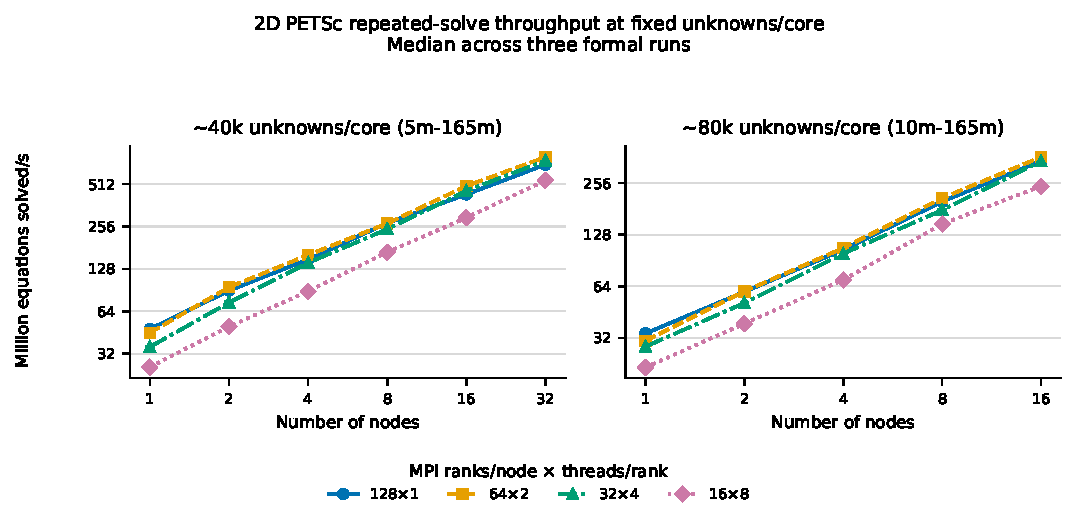
\includegraphics[width=\textwidth]{ksp2d_throughput_vs_nodes}
  \caption{Median 2D repeated-solve throughput along the two unknowns/core chains.
  Whiskers show the observed range of three formal runs. All layouts use 128 cores per
  node, so a fixed node count means a fixed core count.}
  \label{fig:2d-throughput}
\end{figure}

\begin{figure}[htbp]
  \centering
  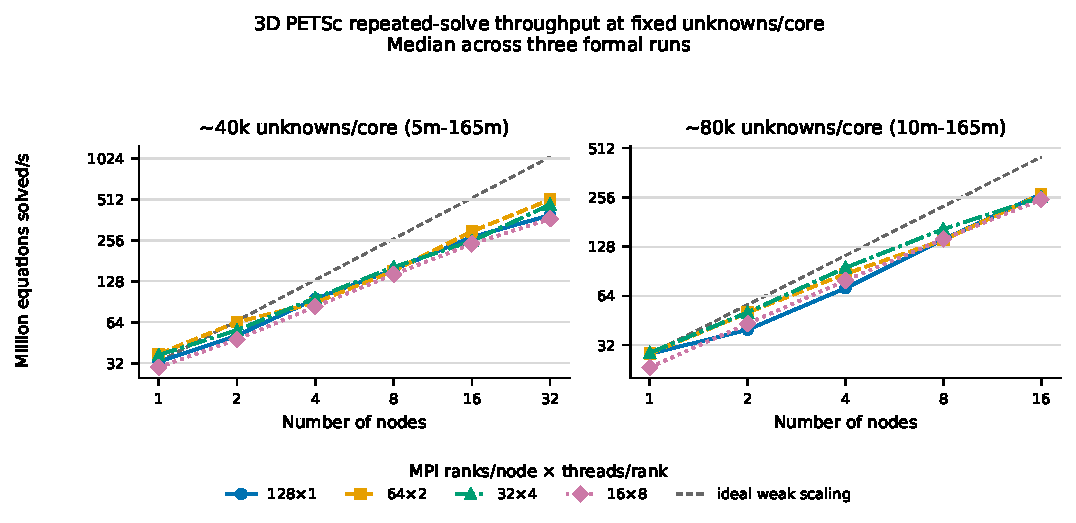
\includegraphics[width=\textwidth]{ksp3d_throughput_vs_nodes}
  \caption{Median 3D repeated-solve throughput along the two unknowns/core chains.
  Whiskers show the observed range of three formal runs.}
  \label{fig:3d-throughput}
\end{figure}

\section{Fixed-size runtime grids}
\label{app:strong20m-grids}

\Cref{sec:strong20m} presented these two campaigns as curves. \Cref{fig:2d-strong20m}
showed the four 2D layouts falling together across the whole range and still falling at 32
nodes, and \Cref{fig:3d-strong20m} showed the 3D layouts separating instead, as three of
the four reached a minimum and turned upward.

\Cref{tab:strong20m-grid-2d} and \Cref{tab:strong20m-grid-3d} give every point behind
those two figures. Chapter 4 tabulates only the fastest
layout at each node count and the 32-node endpoint, so these grids are what an examiner
needs to check a runtime read off either figure. The last two columns state what the
figures show as a shape: the speedup each layout gains over the final doubling, and the
largest three-repeat spread it showed at any node count on the curve.

The 2D grid falls monotonically in all four rows. No layout has reached its minimum
within 32 nodes, but the final doubling returns 1.11 to $1.39\times$ rather than the
$2\times$ of the earlier steps, so the curves are flattening even though none has turned.
The 3D grid turns upward in three rows out of four, at eight nodes for $128\times1$ and
16 nodes for $64\times2$ and $32\times4$. The last-doubling column is below 1.00 for
exactly those layouts that are getting slower.

\begin{table}[htbp]
  \centering
  \caption{2D fixed-size campaign, $4500^2$ and 20.25M unknowns, median seconds per solve
  over three runs at every layout and node count. The final columns give the 16-to-32-node
  speedup and the largest observed three-repeat spread on that row. All layouts fill the
  node, so 32 nodes is 4096 cores in every row. Iteration counts range from 9 to 11.}
  \label{tab:strong20m-grid-2d}
  \begin{tabular}{lrrrrrrrr}
    \toprule
    & \multicolumn{6}{c}{Median s/solve at $N$ nodes} & & \\
    \cmidrule(lr){2-7}
    Layout & 1 & 2 & 4 & 8 & 16 & 32 & 16$\to$32 & Spread \\
    \midrule
    $128\times1$ & 0.7704 & 0.3399 & 0.1351 & 0.0558 & 0.0313 & 0.0282 & 1.11 & 7.9\% \\
    $64\times2$ & 0.8260 & 0.3365 & 0.1265 & 0.0541 & 0.0348 & 0.0277 & 1.26 & 2.7\% \\
    $32\times4$ & 0.8839 & 0.3944 & 0.1465 & 0.0632 & 0.0388 & 0.0317 & 1.22 & 10.8\% \\
    $16\times8$ & 1.1325 & 0.5223 & 0.2272 & 0.0973 & 0.0568 & 0.0409 & 1.39 & 4.8\% \\
    \bottomrule
  \end{tabular}
\end{table}

\begin{table}[htbp]
  \centering
  \caption{3D fixed-size campaign, $273^3$ and 20.35M unknowns, median seconds per solve
  over three runs at every layout and node count. Columns as in
  \Cref{tab:strong20m-grid-2d}. A 16-to-32-node figure below 1.00 means the layout is
  slower at 32 nodes than at 16. Iteration counts are 6 or 7 throughout.}
  \label{tab:strong20m-grid-3d}
  \begin{tabular}{lrrrrrrrr}
    \toprule
    & \multicolumn{6}{c}{Median s/solve at $N$ nodes} & & \\
    \cmidrule(lr){2-7}
    Layout & 1 & 2 & 4 & 8 & 16 & 32 & 16$\to$32 & Spread \\
    \midrule
    $128\times1$ & 0.9066 & 0.5149 & 0.2208 & 0.0997 & 0.1776 & 0.2599 & 0.68 & 4.2\% \\
    $64\times2$ & 0.8288 & 0.4041 & 0.2342 & 0.0936 & 0.0748 & 0.1703 & 0.44 & 3.2\% \\
    $32\times4$ & 0.8022 & 0.4028 & 0.2145 & 0.1192 & 0.0652 & 0.0747 & 0.87 & 11.1\% \\
    $16\times8$ & 0.9707 & 0.4718 & 0.2475 & 0.1330 & 0.1017 & 0.0681 & 1.49 & 7.6\% \\
    \bottomrule
  \end{tabular}
\end{table}
% VERIFIED 2026-08-05 by analysis/scripts/strong_scaling_20m/emit_runtime_grid.py ->
%   analysis/data/nproc_{2d,3d}_libsci/tables/strong_scaling_20m/
%   strong_scaling_20m_runtime_grid.csv, which reads the same
%   strong_scaling_20m_summary.csv that draws fig:2d-strong20m and fig:3d-strong20m.
%   The script also prints these tabular rows, so they are not typed by hand. Spread is
%   the row maximum of runtime_spread, (max - min) / median over the three repeats.

\chapter{Full log\_view Excerpts}
\label{app:logs}
% Optional: before/after RepeatedSolves log_view listings referenced in Ch6.

\end{document}
